\documentclass[11pt]{cernrep}
\usepackage{graphicx,epsfig}
\usepackage{amsmath}
\usepackage{xspace}
\usepackage[dvipsnames]{xcolor}
\bibliographystyle{lesHouches}

% newcommands (for now)
\newcommand{\GoSam}{\protect\textsc{GoSam}\xspace}
\newcommand{\Hej}{\protect\textsc{Hej}\xspace}
\newcommand{\Herwig}{\protect\textsf{Herwig~7.1}\xspace}
\newcommand{\HNNLO}{\protect\textsc{Hnnlo}\xspace}
\newcommand{\HqT}{\protect\textsc{HqT}\xspace}
\newcommand{\MGaMC}{\protect\texttt{Madgraph5\_aMC@NLO}\xspace}
\newcommand{\Powheg}{\protect\texttt{POWHEG}\xspace}
\newcommand{\PowhegBox}{\protect\texttt{POWHEG-BOX}\xspace}
\newcommand{\Pythia}{\protect\textsc{Pythia}\xspace}
\newcommand{\Sherpa}{\protect\textsc{Sherpa}\xspace}
\newcommand{\Rivet}{\protect\textsc{Rivet}\xspace}

\newcommand{\Minlo}{\protect\textsc{MiNlo}\xspace}
\newcommand{\Loopsim}{\protect\textsc{LoopSim}\xspace}
\newcommand{\NLOPS}{\protect\textsc{NloPs}\xspace}
\newcommand{\NNLOPS}{\protect\textsc{NnloPs}\xspace}
\newcommand{\MCatNLO}{\protect\textsc{Mc@Nlo}\xspace}
\newcommand{\MEPSatNLO}{\protect\textsc{MePs@Nlo}\xspace}

\def\Todo#1{{$\bullet$~\color{BrickRed}\textbf{#1}}}
\newcommand{\gev}{\:\ensuremath{\text{GeV}}\xspace}
\newcommand{\antikt}{\ensuremath{\text{anti-}k_\text{T}}\xspace}


\begin{document}

% find a catchy title, this is just a filler
\title{A comparative study of Higgs boson plus jets production in gluon fusion}

\author{
  J.\ Andersen$^1$,
  S.\ Badger$^2$,
  K.\ Becker$^3$,
  J.\ Bellm$^1$,
  R.\ Boughezal$^4$,
  G.\ Falmagne$^{5,6}$,
  R.\ Frederix$^7$,
  M.\ Grazzini$^8$,
  N.\ Greiner$^8$,
  S.\ H\"oche$^6$,
  J.\ Huston$^9$,
  X.\ Liu$^{10}$,
  G.\ Luisoni$^{11}$,
  F.\ Petriello$^{4,12}$,
  S.\ Pl\"atzer$^{1,13}$,
  P.\ Schichtel$^1$,
  M.\ Sch\"onherr$^8$,
  F.\ Tackmann$^{14}$,
  E.\ Vryonidou$^{15}$,
  J.\ Winter$^8$
}
\institute{
  $^1$ Institute for Particle Physics Phenomenology, Durham University\\
  $^2$ Edinburgh\\
  $^3$ Oxford\\
  $^4$ Argonne National Laboratory, Argonne, USA\\
  $^5$ ENS Cachan, Universit\'e Paris--Saclay\\
  $^6$ SLAC National Accelerator Laboratory, Stanford University\\
  $^7$ Physik Department T31, Technische Universit\"at M\"unchen\\
  $^8$ Physik-Institut, Universit\"at Z\"urich\\
  $^9$ Michigan State University\\
  $^{10}$ Maryland Center for Fundamental Physics, University of Maryland, Maryland, USA\\
  $^{11}$ CERN\\
  $^{12}$ Department of Physics \& Astronomy, Northwestern University, Evanston, USA\\
  $^{13}$ School of Physics and Astronomy, University of Manchester\\
  $^{14}$ DESY\\
  $^{15}$ Centre for Cosmology, Particle Physics and Phenomenology
          (CP3), Universit\'e catholique de Louvain
}

\maketitle

\begin{abstract}
  We look at $pp\to h + \text{jets}$ production.
\end{abstract}

\subsection{INTRODUCTION}
\label{sec:hjetscomp:intro}

There has been a great deal of progress in
the attack on the Les Houches precision wish list. Such higher order
calculations are needed for the full exploitation of precision LHC
measurements. It is more common in ATLAS and CMS, however, to compare
to predictions involving parton shower Monte Carlos, often
supplemented with matrix element information at leading order (LO) and
next-to-leading order (NLO). Such frameworks allow for the generation
of fully exclusive final states, often more amenable to comparisons
with experimental data. There are a number of such matrix-element plus
parton-shower (ME+PS) frameworks used by the LHC collider experiments,
as can be seen from the predictions in this section. But the higher
(fixed) order calculations often provide the highest precision. It is
thus important to understand: (1) the degree to which the various
ME+PS predictions agree with each other, (2) how well the ME+PS
predictions agree with fixed-order predictions and (3) the impact of
Sudakov regions\,\footnote{By Sudakov region, we refer to kinematic
situations where there is a severe restriction on phase space for
gluon emission, such as the Higgs boson transverse momentum
distribution at low $p_\perp$.} and/or the imposition of jet
vetoes/binning on both fixed-order and ME+PS predictions.  We come to
these comparisons with several expectations: outside of Sudakov regions, the
influence of parton showering/resummation should be mild, and cross
sections that are fairly inclusive (such as the lead-jet transverse
momentum distribution for $h$~+~$\ge1$ jet) should not be subject to
large jet veto logs.

The production of a Higgs boson through gluon--gluon fusion is an
excellent testing ground for such comparisons, both because of the
importance of the process, and the enhanced rate for additional jet
production associated with gluon--gluon fusion. This process of
comparison was started in Les Houches
2013~\cite{AlcarazMaestre:2012vp}, with comparisons of various
predictions for $h$~+~$\ge2$ jets from gluon--gluon fusion, a critical
background for the measurement of vector boson fusion. Here, in this
contribution to the Les Houches 2015 proceedings, we extend that study
to more observables, for a variety of jet multiplicities, and with
comparisons to fixed-order predictions as well as to ME+PS frameworks.

To allow for as standardized a comparison as possible, a group of
generation parameters were agreed upon. MMHT2014 NLO PDFs (and the
NNLO version for the NNLO calculations) were to be used, with a
central value of $\alpha_\mathrm{s}(m_Z)=0.118$.  
Variations of scale choice are allowed; however, they
should reproduce a scale of $\tfrac{1}{2}m_h$ in the zero-jet limit.

Alas, in some cases, there are deviations from these standards. These
will be noted where present, and the impact on the comparisons will be
discussed.  The Higgs boson was left undecayed. Jets were reconstructed 
with the anti-$k_T$ jet clustering algorithm \cite{Cacciari:2008gp} using
$R=0.4$, and a transverse momentum constraint of $30\gev$ was imposed,
along with a rapidity cut of $\eta(j)<|4.4|$.  To provide a common
framework for the display of the results, a Rivet
routine~\cite{Buckley:2010ar,webpage} was created and distributed to each group
providing a prediction.

In this contribution, predictions have been made with fixed-order
calculations at NLO for $pp\to h+1,2,3j$ with standard scale choices 
and the \Minlo approach including Sudakov factors (using \GoSam in 
comnbination with \Sherpa, cf.\ Secs.\ 
\ref{sec:hjetscomp:tools:fo:hnj}-\ref{sec:hjetscomp:tools:fo:hnjminlo}), 
at approximate NNLO (using the \Loopsim approach, cf. Sec.\ 
\ref{sec:hjetscomp:tools:fo:hnjloopsim}) and full NNLO for $pp\to h$ 
(using \Sherpa, cf.\ Sec.\ \ref{sec:hjetscomp:tools:fo:sherpa}) and 
$pp\to h+j$ (using the results of the BFGLP group, cf.\ 
\ref{sec:hjetscomp:tools:fo:BFGLP}). These are compared to explicit 
high-precision resummation calculations for observables of interest, 
i.e.\ the inclusive Higgs boson transverse momentum (using \HqT, cf.\ 
Sec.\ \ref{sec:hjetscomp:tools:ares:hqt}) and jet-vetoed zero jet 
cross section (using the results of the STWZ group, cf.\ Sec.\ 
\ref{sec:hjetscomp:tools:ares:jvres}), as well as to the generic 
parton shower matched predictions of inclusive Higgs boson production 
at NNLO (using \Powheg and \Sherpa, cf.\ Secs.\ 
\ref{sec:hjetscomp:tools:nnlops:powheg} and 
\ref{sec:hjetscomp:tools:nnlops:sherpa}) and the multijet merged 
predictions (provided by \MGaMC, \Herwig and \Sherpa, cf.\ Secs.\ 
\ref{sec:hjetscomp:tools:mc:mgamc}-\ref{sec:hjetscomp:tools:mc:sherpa}), 
using NLO matrix element information for up to two (three) jets (\Sherpa). 
For observables requiring the presence of at least two jets, results 
obtained resumming BFKL-type logarithms (using \Hej, cf.\ Sec.\ 
\ref{sec:hjetscomp:tools:bfkl:hej}) are added. 
Sec.\ \ref{sec:hjetscomp:results} then presents the results in detail 
for a multitude of relevant observables.

\subsection{TOOLS}
\label{sec:hjetscomp:tools}

% \subsection{Fixed-order computations}
\label{sec:hjetscomp:tools:fo}
\subsubsection{NLO calculation of $pp\to h+1,2,3\,\text{jets}$}
\label{sec:hjetscomp:tools:fo:hnj}

We compute $h+1$ jet, $h+2$ jets and
$h+3$ jets at NLO in QCD in the infinite top mass limit 
\cite{vanDeurzen:2013rv,Cullen:2013saa,Greiner:2015jha}
using \textsc{Sherpa}~\cite{Gleisberg:2008ta} and
\textsc{GoSam}~\cite{Cullen:2011ac,Cullen:2014yla}, linked via the
interface defined in the Binoth Les Houches
Accord~\cite{Binoth:2010xt,Alioli:2013nda}.
The one-loop amplitudes are generated with \textsc{GoSam} employing
\textsc{QGraf}~\cite{Nogueira:1991ex},
\textsc{Form}~\cite{Vermaseren:2000nd,Kuipers:2012rf} and
\textsc{Spinney}~\cite{Cullen:2010jv}, The reduction of the loop
integrals is performed using
\textsc{Ninja}~\cite{Mastrolia:2012bu,vanDeurzen:2013saa,Peraro:2014cba},
\textsc{Golem95}~\cite{Heinrich:2010ax,Binoth:2008uq,Cullen:2011kv}
and \textsc{OneLoop}~\cite{vanHameren:2010cp} for the evaluation of
the scalar integrals.
The calculation of tree-level matrix elements for the Born and the
real emission contribution as well as the subtraction terms in the
Catani-Seymour approach~\cite{Catani:1996vz} have been done within
\textsc{Sherpa} using the matrix element generator
\textsc{Comix}~\cite{Gleisberg:2008fv}.

The computation is performed for a Higgs boson with mass
$m_h=125\,\gev$, which is left undecayed. We used the 
\texttt{MMHT2014nlo68clas118} PDF set. We present results 
obtained by processing events pre-generated and
stored in form of \textsc{Root} Ntuples as described
in~\cite{Bern:2013zja}. Theoretical
uncertainties are estimated by varying renormalization and
factorization scales by factors of $\tfrac{1}{2}$ and $2$ 
around the central scale
\begin{equation}
  \mu_0 \;=\; \tfrac{1}{2}\,\sqrt{m_{h}^2+\sum p_{T,j_i}^2}\;,
\end{equation}
where $i$ runs over all identified jets.
This scale was chosen to facilitate comparison with the $h+1$ jet NNLO
calculation of Sec.\ \ref{sec:hjetscomp:tools:fo:BFGLP}.


\subsubsection{\textsc{MiNLO} calculation of $pp\to h+1,2,3\,\text{jets}$}
\label{sec:hjetscomp:tools:fo:hnjminlo}

Reprocessing the \textsc{Root} Ntuples of Sec.\ 
\ref{sec:hjetscomp:tools:fo:hnj}, for the first time in these 
proceedings we present fixed order NLO results evaluated with a
\textsc{MiNLO}~\cite{Hamilton:2012np} scale chioce, as implemented in
\textsc{Sherpa}. Events are read-in by \textsc{Sherpa}, which applies
the \textsc{MiNLO} prescription event by event. As a \textsc{MiNLO}
core scale we choose
\begin{equation} \label{eq:hthatprime}
  \mu_\text{core}^\text{\textsc{MiNLO}}
  \;=\;\tfrac{1}{2}\,\hat{H}^\prime_T
  \;=\;\tfrac{1}{2}\left(\sqrt{m_h^{2}+p_{T,h}^{2}}
       +\sum_{i}p_{T,i}^{}\right)\,
\end{equation}
where $i$ runs over all partons of the identified core.

\subsubsection{\textsc{LoopSim} merged nNLO calculation of 
               $pp\to h+(1,2)\,\text{jets}$ and $pp\to h+(2,3)\,\text{jets}$}
\label{sec:hjetscomp:tools:fo:hnjloopsim}

The fixed order Ntuples produced by \textsc{GoSam}{}+\textsc{Sherpa} 
detailed in Sec.\ \ref{sec:hjetscomp:tools:fo:hnj} can be combined 
using the \Loopsim \cite{Rubin:2010xp} procedure to make an approximate 
NNLO prediction, labelled nNLO in the following, which is missing the 
double virtual corrections but captures much of the double unresolved 
radiation contributions. There is a cut-off dependence on the additional 
real radiation since the fixed order Ntuples where generated with a jet 
$p_T>25$ GeV. The \Loopsim procedure uses a flavour sensitive 
$k_T$-algorithm where a jet radius of $R=1$ was used. All other 
parameters and scales were chosen the same as in the fixed order case 
with the exception of the PDF where the NNLO PDF set 
\texttt{MMHT2014nnlo68cl} was used.


\subsubsection{Fixed-order calculation for $pp\to h$}
\label{sec:hjetscomp:tools:fo:sherpa}


\subsubsection{NNLO calculation of $pp\to h+j$}
\label{sec:hjetscomp:tools:fo:BFGLP}

The NNLO calculation for Higgs production in association with one or 
more jets is obtained using the $N$-jettiness subtraction 
scheme~\cite{Boughezal:2015dva,Gaunt:2015pea}.  The application of 
this technique to obtain the full NNLO result for Higgs+jet, and its 
validation against another calculation using sector-improved residue 
subtraction~\cite{Boughezal:2015dra}, was described in 
\cite{Boughezal:2015aha}.  In this study we adapt the dynamical scale choice
%
\begin{equation}
  \mu_0 = \tfrac{1}{2}\,\sqrt{m_{h}^2+\sum p_{T,j_i}^2}
\end{equation}
%
for both the renormalization and factorization scales, where the sum 
runs over all reconstructed jets.  This dynamical scale correctly 
captures the characteristic energy throughout the entire kinematic 
range.  To estimate the theoretical uncertainties we equate $\mu_R$ 
and $\mu_F$ and vary them in the range $\mu_0/2 \leq \mu_{R,F} \leq 2 \mu_0$.  
We use \texttt{CT14nnlo} parton distribution functions 
\cite{Dulat:2015mca}.  Jets are reconstructed using the anti-$k_T$ algorithm 
with $R=0.4$, subject to the requirements $p_T>30$ GeV and $|\eta|<4.4$.


% \subsection{Analytic resummations}
\label{sec:hjetscomp:tools:ares}
\subsubsection{\HqT}
\label{sec:hjetscomp:tools:ares:hqt}

\HqT \cite{Bozzi:2005wk,deFlorian:2011xf} is a numerical program which 
combines the exact fixed order calculation of the transverse momentum 
spectrum valid at large $q_T$ at ${\cal O}(\alpha_S^4)$ with the 
resummation of the logarithmically enhanced contributions at small 
transverse momenta at next-to-next-to-leading logarithmic accuracy.
The calculation is performed according to the formalism of 
\cite{Catani:2000vq,Bozzi:2005wk} and it implements a unitarity 
constraint such that, upon integration over $q_T$, the inclusive 
NNLO cross section is recovered. The results are valid in the large 
$m_{top}$ approximation. As any perturbative QCD computation in hadron 
collisions, the results depend on the factorization ($\mu_F$) and 
renormalization ($\mu_R$) scales. In addition, the resummation procedure 
introduces an additional scale, dubbed \lq\lq resummation scale\rq\rq\ 
($Q$). The three scales must be chosen of the order of the hard scale 
of the process, $m_h$. The numerical results presented here are obtained 
by using \HqT-2.0 with $\mu_F=\mu_R=Q=\tfrac{1}{2}\,m_h$ GeV as central scale choice. 
The procedure to estimate perturbative uncertainties is to perform 
independent variations of $\mu_F$, $\mu_R$ and $Q$ around the central 
value by a factor of 2 with the constraints $\tfrac{1}{2} < \mu_F/\mu_R < 2$ and 
$\tfrac{1}{2} <Q/\mu_R<2$.
\subsubsection{\Resbos}
\label{sec:hjetscomp:tools:ares:resbos}

\Resbos is the updated version of \textsc{ResBos} \cite{Balazs:1997xd}, 
which resums the effect of multiple soft gluon radiation to all orders 
in the strong coupling via the $q_T$ resummation formalism proposed by 
Collins-Soper-Sterman \cite{Collins:1984kg}. The \Resbos prediction 
for inclusive Higgs boson production via the gluon fusion process 
includes the full NNLO QCD corrections in the total rate (similar to 
the setup of a \HNNLO calculation) and 
the NLO contribution to the Higgs boson distribution at large transverse 
momentum ($q_T$) \cite{Glosser:2002gm}. In this calculation, we include 
NNLL accuracy in the Sudakov factor and NNLO accuracy in the Wilson coefficient functions 
of the resummed piece, which is matched to the perturbative piece, 
evaluated at the NLO, in the high $q_T$ region \cite{Wang:2012xs}. The 
renormalization and resummation scales have been varied by a factor 
of 2 around the central value of $\tfrac{1}{2}m_h$, with the 
non-perturbative parameters needed for the $q_T$ resummation calculation 
taken to be the same values as those in \cite{Wang:2012xs}. The 
\texttt{MMHT2014nnlo68cl} PDF set has been used.

The \Resbos prediction of inclusive Higgs plus jet production via 
gluon fusion is based on the transverse momentum dependent (TMD) 
resummation formalism, in the Collins 2011 scheme \cite{Collins:2011zzd}.
The prediction includes the NLL Sudakov factor and the NLO inclusive rate in the 
resummed piece which is matched to NLO QCD prediction in the large 
$q_T$ region \cite{Sun:2016kkh}. Here, $q_T$ denotes the transverse 
momentum of the Higgs boson and jet system. Thus, the total 
inclusive rate of Higgs plus jet production, applying a minimum cut on the jet transverse 
momentum, will agree well with that given by the NLO calculation, such 
as produced by MCFM \cite{Campbell:2010ff}. 
The resummation calculation provides a better description for kinematic distributions 
of Higgs boson and jet when they are almost back-to-back. In this 
calculation, we have fixed the resummation scale to be the jet 
transverse momentum ($p_T(j)$), as suggested in \cite{Sun:2016kkh}, 
and have varied the renormalization scale by a factor of 2 around its 
central value $\tfrac{1}{2}m_h$, with the non-perturbative parameters 
needed for the TMD resummation calculation taken to be the same values 
as those in \cite{Sun:2016kkh}. The jets are defined based on the \antikt 
algorithm using $R = 0.4$; they furthermore have to obey the criteria that 
$p_T(j) > 30$ GeV and its rapidity $|\eta(j)| < 4.4$. The 
\texttt{MMHT2014nnlo68cl} PDF set has been used.


\subsubsection{Jet veto resummation}
\label{sec:hjetscomp:tools:ares:jvres}

To resum the $p_\perp$ spectrum of the leading jet as well as the exclusive $0$-jet
(jet-vetoed) cross section, the STWZ predictions~\cite{Stewart:2013faa} utilize
the soft-collinear effective theory (SCET) formalism for jet-veto resummation at
hadron colliders as developed in \cite{Stewart:2009yx, Berger:2010xi,
Tackmann:2012bt, Stewart:2013faa}. The results are obtained in the HEFT 
limit, taking $m_\text{top}\to\infty$.
Jets are defined with a jet radius of $R = 0.4$ and without any cut on the jet
rapidity. The \texttt{MMHT2014nnlo68cl} PDFs are used. The calculation is carried out to
NNLL$'+$NNLO order. The resummation is performed by renormalization group
evolution in virtuality and rapidity space in SCET. The NNLL$'$ resummation
includes the RG evolution at next-to-next-to-leading logarithmic order together
with the full NNLO singular matching correction, thus incorporating all two-loop
virtual and singular real-emission contributions in the resummation. This allows
to perform the matching to the full NNLO result by adding purely nonsingular
corrections to the resummed contributions, and to achieve a smooth transition to
the fixed-order result simply by turning off the RG evolution using profile
scales~\cite{Ligeti:2008ac, Abbate:2010xh}. The perturbative uncertainties are
estimated by varying the relevant virtuality and rapidity renormalization scales
using profile scale variations, which has been established as a reliable method
to assess perturbative uncertainties in resummed predictions. We evaluate
separate fixed-order and resummation uncertainties which are added in
quadrature~\cite{Berger:2010xi, Stewart:2011cf, Stewart:2013faa}.
The predictions use a complex value for the hard scale $\mu_H = -i \mu_{FO}$ where
$\mu_{FO} = m_h$ is the fixed-order scale, which allows to resum large virtual
corrections in the $gg\to h$ form factor in both the 0-jet limit and the
inclusive cross section. This scale choice results in a similar 
inclusive cross section compared to a standard NNLO calculation with 
$\mu_R=\mu_F=\tfrac{1}{2}m_h$. The uncertainty related to this resummation is
estimated by varying the phase of $\mu_H$ and is also added in quadrature.



% \subsection{NNLOPS matched simulations}
\label{sec:hjetscomp:tools:nnlops}
\subsubsection{\Powheg \NNLOPS}
\label{sec:hjetscomp:tools:nnlops:powheg}

One of the generators under investigation is the \NNLOPS prediction 
of Higgs boson production via gluon fusion~\cite{Hamilton:2013fea}.
To produce this sample, the Higgs-boson-plus-jet \Minlo~\cite{Hamilton:2012np} 
predictions generated with \PowhegBox{}\texttt{-v2}~\cite{Campbell:2012am} 
are combined with an NNLO accurate analytical calculation by the 
program \HNNLO (v.2.0)~\cite{Catani:2007vq,Grazzini:2008tf,Grazzini:2013mca} 
following the instructions in \cite{Hamilton:2013fea}. Here, the rapidity 
spectrum of the Higgs boson of the \Powheg \texttt{HJ} \Minlo prediction 
is reweighted with the spectrum from \HNNLO, while ensuring that NLO 
precision is kept for the kinematic properties of the first additional jet. 
In the generation and the \HNNLO calculation, the default parameters are 
set as follows, in particular the renormalization and factorization scales 
have been set to $\mu_R = \mu_F = \tfrac{1}{2}\,m_h$ and the 
\texttt{MMHT2014nnlo68cl} \cite{Harland-Lang:2014zoa} has been used. 
To evaluate the uncertainties in the choice of the renormalization and 
factorization scales, the 21-point scale variations described in detail 
in \cite{Hamilton:2013fea} are evaluated.
The \NNLOPS sample is showered with \Pythia~8 (v.8.253) \cite{Sjostrand:2014zea} 
using the \texttt{NNPDF} \texttt{2.3} leading-order PDF set~\cite{Ball:2012cx} 
and the A14 tune~\cite{ATL-PHYS-PUB-2014-021}. 

The variation of the renormalization scale also varies consistently the 
resummation scale in the Sudakov form factor of the \Minlo 
procedure~\cite{Hamilton:2012rf}. Other resummation properties are not 
varied in this simulation. 


\subsubsection{\Sherpa \NNLOPS}
\label{sec:hjetscomp:tools:nnlops:sherpa}

A second NNLO prediction matched to a parton shower is investigated 
in this study. The computation is performed in the \textsc{uN$^2$loPs} 
method~\cite{Hoeche:2014aia,Hoche:2014dla}, which is based on the 
\textsc{uNloPs} algorithm for merging inclusive NLO matched calculations 
of varying jet multiplicity, while leaving their total cross sections 
unchanged~\cite{Lonnblad:2012ix,Lonnblad:2012ng}. The event samples 
used in this comparison were generated with an implementation of the 
\textsc{uN$^2$loPs} matching scheme in the event generator \Sherpa. The 
NNLO prediction needed for the matching is computed within \Sherpa itself, 
using a $q_T$ cutoff method~\cite{Gao:2012ja}, for details see 
\cite{Hoeche:2014aia,Hoche:2014dla}. We used a parton shower based 
on Catani-Seymour dipole factorization~\cite{Schumann:2007mg,Hoeche:2009xc},
which has been matched to the Higgs plus jet NLO calculation using 
the S-MC@NLO method~\cite{Hoeche:2011fd,Hoeche:2012ft}. Renormalization 
and factorization scales for the fixed-order calculation have been 
set to $\mu_R = \mu_F = \tfrac{1}{2}\,m_h$, and the the parton shower 
starting scale is set to the same value. The \texttt{MMHT2014nnlo68cl} 
PDF set \cite{Harland-Lang:2014zoa} has been used throughout.


% \subsection{Multijet merged calculations}
\label{sec:hjetscomp:tools:mc}
\subsubsection{\MGaMC}
\label{sec:hjetscomp:tools:mc:mgamc}

Higgs production in gluon fusion, in association with multiple jets,
is generated with \MGaMC \cite{Alwall:2014hca}~at NLO
accuracy using the following commands
\begin{verbatim}
  import model HC_NLO_X0_UFO-heft
  generate p p > x0 /t [QCD] @0
  add process p p > x0 j /t [QCD] @1
  add process p p > x0 j j /t [QCD] @2
  output MG5aMC_FxFx_Hjets
\end{verbatim}
The first command loads the model that includes the Higgs boson
effective coupling to gluons in the $m_t\to\infty$ limit. This model
can be found on the
FeynRules~\cite{Alloul:2013bka}~website\footnote{\texttt{http://feynrules.irmp.ucl.ac.be}}
and was originally created for the studies in
\cite{Demartin:2014fia}. In this model, the Standard Model Higgs
boson is called `\texttt{x0}', and therefore the second to fourth
commands generate this boson in association with 0, 1 and 2 jets,
respectively. The model, and therefore also the definitions of
\texttt{p} and \texttt{j}, are in the 5 flavour scheme. The
`\texttt{/t}' syntax is needed to remove the explicit top quark
contributions from the loops (they are already integrated out in the
effective Higgs-gluon vertices). By setting the parameter
\texttt{ickkw} to \texttt{3} in the \texttt{run\_card.dat}, the FxFx
merging~\cite{Frederix:2012ps}~is turned on. The LHE events are
matched to the \Pythia 8 (v.210) parton
shower~\cite{Sjostrand:2014zea}, using the FxFx interface also used in
\cite{Frederix:2015eii}. As central choices for the factorisation
and renormalisation scales we use the default value in the
\MGaMC code, which, in the context of FxFx merging, is
roughly given by the transverse energy of the Higgs boson, after the
partons entering the matrix elements have been clustered to a $pp \to h
j$ configuration. $pp\to h$ configurations thus are calculated using 
$m_h$ as the scale. The central merging scale is taken to be 35 GeV,
while the variations include 25 GeV and 50 GeV. These scales include 
values both below as well as above the default minimal jet transverse
momentum used in the analysis and should therefore cover the complete
range of uncertainties coming from the merging.  The uncertainty band
is computed by varying the factorisation and renormalisation scales by
a factor of 2 up and down from the central value, using the reweighting
technique as described in \cite{Frederix:2011ss}, for each of the
three choices of merging scales. It is therefore obtained
as the bin-by-bin envelope of $3 \times 3 \times 3 = 27$ individual
values. This is similar to what is done in
\cite{Frederix:2015eii}---apart from the uncertainties coming
from the parton distribution function, which are not taking into
account here. Throughout the \texttt{MMHT2014nlo68cl} PDF set with 
$\alpha_\mathrm{s}(m_Z)=0.12$ has been used, as compared to the canonical choice
of $0.118$. There is a partial cancellation between the effects of the larger scale choice
and the larger  value of $\alpha_\mathrm{s}(m_Z)$, but for most of the comparisons, 
when there are notable differences, they can be traced to the larger scale choice of \MGaMC. 

\subsubsection{\Herwig}
\label{sec:hjetscomp:tools:mc:herwig}

We provide predictions from NLO merging of $h+0,1,2$ jets at NLO and $h+3,4$
jets at LO in the Higgs effective theory. The merging is carried out with the
\Herwig \ \cite{Bellm:2015jjp} dipole shower module based on
\cite{Platzer:2009jq,Platzer:2011bc}, in a modified version of the algorithms
set out in \cite{Platzer:2012bs,Lonnblad:2012ix}, and implemented in
\cite{Bellm:thesis,Bellm:2016xxx}. The merging implementation will become
publicly available in \textsf{Herwig~7.1}. We use \textsf{MadGraph~5}
\cite{Alwall:2011uj} generated amplitudes together with \textsf{ColorFull}
\cite{Sjodahl:2014opa} for the point-by-point evaluation of tree-level type
objects (tree level matrix elements squared, colour- and spin-correlated
matrix elements), and \textsf{OpenLoops} \cite{Cascioli:2011va} for the
evaluation of Born/one-loop interferences.  Subtraction terms and their
integrated counter-parts, phase space generation, integration and process
bookkeeping is handled by the \textsf{Matchbox} module as outlined in
\cite{Bellm:2015jjp}.

The algorithm we use is a modified, unitarized merging algorithm. We allow
finite, higher-order cross section corrections in higher multiplicity jet
bins, but still choose a unitarization procedure to remove potentially
dangerous, logarithmic enhanced terms in inclusive quantities. Below the
merging scale of $30\ {\rm GeV}$, NLO accuracy of the first additional
emission off each contribution is reached by the standard subtractive
matching. Scales are determined through clustering and the core scale 
is defined as $\mu_R=\mu_F=\tfrac{1}{2}\,m_h$. The shower starting scale 
is set to the same value. The uncertainty band is obtained by variation of 
the renormalization and factorization scales of the hard input processes, 
and is covering all other uncertainties present in the algorithm 
(specifically, merging and shower scale variations).

\subsubsection{Sherpa MEPS@NLO}
\label{sec:hjetscomp:tools:mc:sherpa}


% \subsection{BFKL resummations}
\label{sec:hjetscomp:tools:bfkl}
\subsubsection{\hjetscompHej}
\label{sec:hjetscomp:tools:bfkl:hej}

High Energy Jets (\hjetscompHej) describes hard, wide angle (high energy-)
emissions to all orders and to all multiplicities. The predictions are based
on events generated according to an all-order resummation, merged with
high-multiplicity full tree-level matrix-elements. The explicit all-order summation
is built on an approximation to the n-parton hard scattering matrix element
\cite{Andersen:2009nu,Andersen:2009he,Andersen:2011hs} which becomes exact in
the limit of wide-angle emissions, ensuring leading logarithmic accuracy for
both real and virtual corrections. A first set of sub-leading logarithmic
terms are included by allowing one un-ordered gluon emission from quarks. All
of these logarithmic terms are important when
the partonic invariant mass is large compared to the typical transverse
momentum in the event. This is precisely the situation which arises in
typical \lq\lq VBF\rq\rq\ cuts, including those used in this study.  Matching to the
full tree level accuracy for up to three jets is obtained by supplementing
the resummation with a merging
procedure~\cite{Andersen:2008ue,Andersen:2008gc}.

The implementation of this framework in a fully-flexible Monte Carlo event
generator is available at \texttt{http://hej.web.cern.ch}, and produces
exclusive samples for events with at least two jets.  The predictions include
resummation also for events with up to two un-ordered emissions,
i.e.~contributions from the first sub-leading configurations.

The factorisation and renormalisation scales can be chosen arbitrarily, just
as in a standard fixed-order calculation. Here, we have chosen to evaluate
two powers of the strong coupling at a scale given by the Higgs mass, and for
the central predictions the remaining scales are evaluated at $\mu_R=\tfrac{1}{2}H_T$. Thus,
for the $n$-jet tree-level evaluation, 
\begin{equation}
  \alpha_\mathrm{s}^{n+2}=\alpha_\mathrm{s}^2(m_h)\cdot \alpha_\mathrm{s}^n(\mu_R).
\end{equation}
The scale variation bands shown in the plots here correspond to varying
$\mu_F,\mu_R\in \{\tfrac{1}{2}\mu_c,\,\tfrac{1}{\sqrt{2}}\mu_c,\,\mu_c,$ $\,\sqrt{2}\mu_c,\,2\mu_c\}$ with 
$\mu_c=\tfrac{1}{2}H_T$, but discarding evaluations where any ratio $\mu_F/\mu_R$ or 
$\mu_R/\mu_F$ is bigger than two (which results in a total of 18 variations
around the central scale). The \texttt{CT10nlo} \cite{Lai:2010vv,Gao:2013xoa} parton 
distribution functions were used in the predictions.



\section{RESULTS}
\label{sec:hjetscomp:results}

In the following comparisons, we will typically show the central
values of each prediction on the left (both as absolute predictions
and in ratio to a reference prediction), and a similar comparison of
the predictions with uncertainty bands on the right. The reason for
the former is that with the overlapping uncertainty bands, it can be
difficult to discriminate the behavior of the central predictions. But
it is also useful to compare the uncertainty bands from each
prediction given similar prescriptions for scale variation.  Note that
it is not enough to say that different predictions agree within their
scale uncertainty bands. In most cases, the predictions should be held
to a higher standard, as the scale logs are common to all of the
calculations that are being compared.

In general, the \Powheg \NNLOPS calculation has been chosen as the 
reference of the ratios presented. Only for observables where a 
dedicated calculation exhibits a higher accuracy throughout the 
highest accuracy available is chosen. The rations themselves group 
the predictions by likeness to improve readability. The top most 
ratio shown always compares the \NNLOPS predictions to the reference. 
The second ratio then contains the multijet merged predictions while 
the third ratio collects the fixed order predictions lacking parton 
showering. Additional ratios are added as needed. The BFKL resummation 
of \Hej is inserted into the top ratio where applicable.



\subsection{Inclusive observables}
\label{sec:hjetscomp:results:inclobs}

This section contains observables which characterize the $h+{}$jets
phase space in the most inclusive way. Only the presence of a Higgs
boson is required, with no restrictions on its momentum. We therefore
compare the predictions for the rapidity and transverse momentum
distributions of the Higgs boson. The latter is differentiated into
two cases: its inclusive spectrum and its exclusive spectrum vetoing
the appearance of any jet. Also, to get a first overview on the amount
of jet activity accompanying the Higgs boson production, we look at
the inclusive as well as exclusive cross sections for various jet
multiplicities predicted by the different approaches.

\begin{figure}[t!]
  \centering
  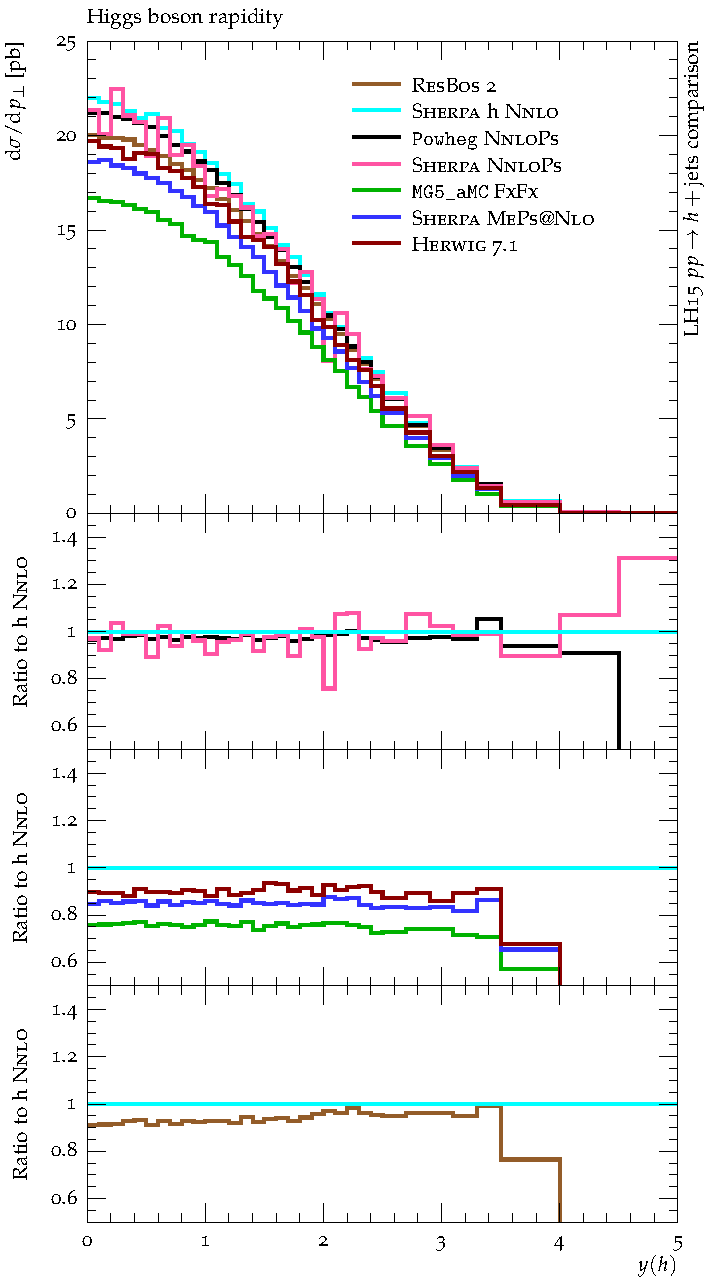
\includegraphics[width=0.47\textwidth]{figures/hjetscomp_u_H_y.pdf}
  \hfill
  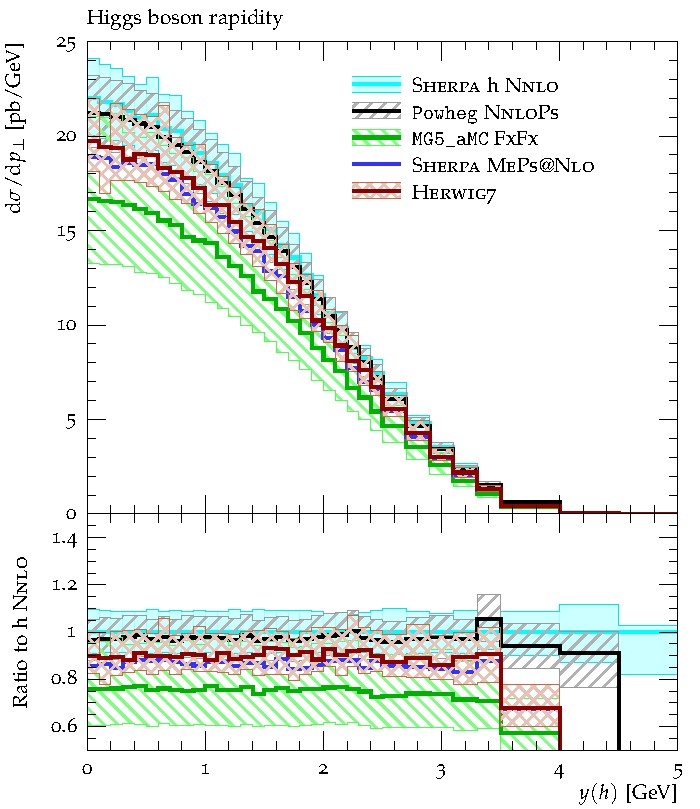
\includegraphics[width=0.47\textwidth]{figures/hjetscomp_H_y.pdf}
  \caption{\label{fig:hjetscomp:results:inclobs:hy}%
    The inclusive Higgs boson rapidity without (left) and with (right)
    uncertainties. To enhance visibility, the \NNLOPS and \MEPSatNLO
    predictions are grouped together and shown with respect to the same reference
    curve in the upper and lower ratio plots, respectively. The
    reference prediction is taken from the NNLO accurate description
    of inclusive $h$ production.}
\end{figure}

We start by examining the inclusive Higgs boson rapidity distribution in
Figure~\ref{fig:hjetscomp:results:inclobs:hy}. While the absolute
predictions are given in the top panel, the plots in the bottom panel
depict the respective ratios to the NNLO prediction. For better
visibility, we have divided the predictions into two groups based on
their simulation type and/or claimed accuracy. The upper ratio plot
contains the NNLO predictions while the lower one shows those obtained
from different strategies to merge matrix elements plus parton showers
at NLO. Overall, we find very good agreement in the description of the
shape of the Higgs boson rapidity distribution. The main source of deviations stems
from the different normalizations given at NNLO or NLO and the
different (core) scale choices. As expected, the \Sherpa \NNLOPS and
\Powheg \NNLOPS results agree well with the fixed order NNLO prediction. 
\Sherpa \NNLOPS' larger fluctuation wrt.\ to \Powheg \NNLOPS' stem from 
it being computed directly rather then reweighted from a NLO computation. 
Consequently, \MGaMC, \Sherpa \MEPSatNLO and \Herwig have slightly lower (NLO)
normalizations.  Here, the \MGaMC scale choice reducing to
$m_h$, rather than $\tfrac{1}{2}m_h$, is clearly noticeable. The upper edge of
the \MGaMC uncertainty band (equal to a scale that reduces to $\tfrac{1}{2}m_h$)
agrees with the central value of the other NLO ME+PS
predictions. There are no major differences in the size of the
uncertainty envelopes, although to some extent, the NNLO scale
uncertainty bands are smaller than those at NLO, as expected. Note
that the NLO-based predictions fall off more rapidly at higher $y$
than the NNLO-based predictions do. This is expected because of the
influence of additional $\ln(1-x)$ corrections present in the
determination of NNLO PDFs. Similar effects can be observed in going
from LO to NLO.

\begin{figure}[t!]
  \centering
  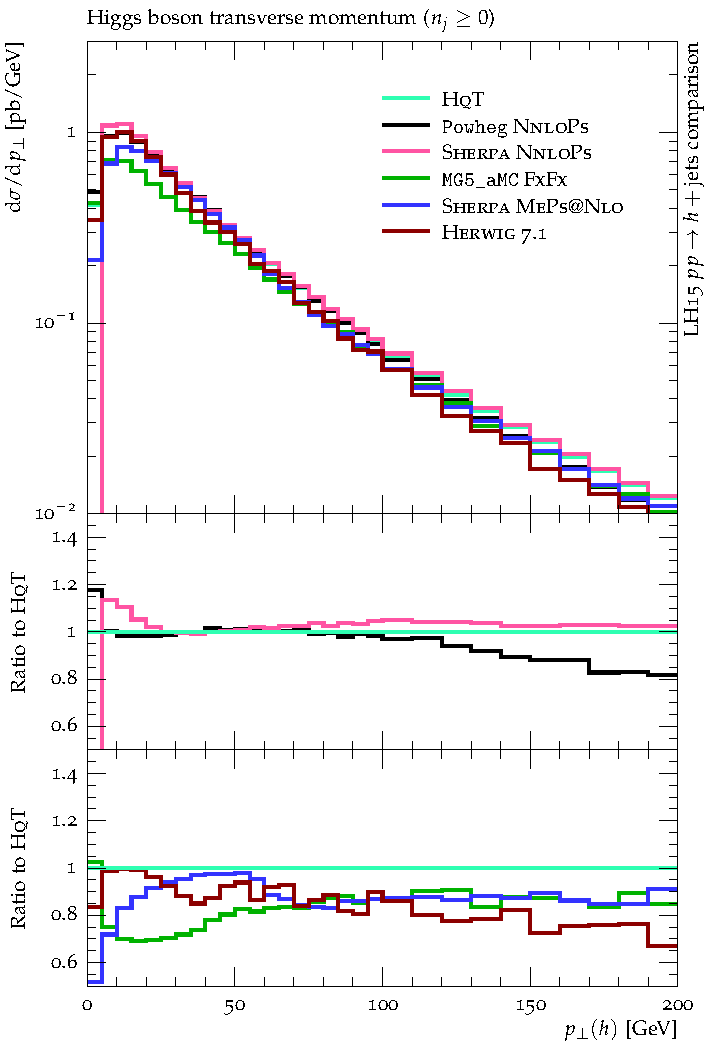
\includegraphics[width=0.47\textwidth]{figures/hjetscomp_u_H_pT_incl.pdf}
  \hfill
  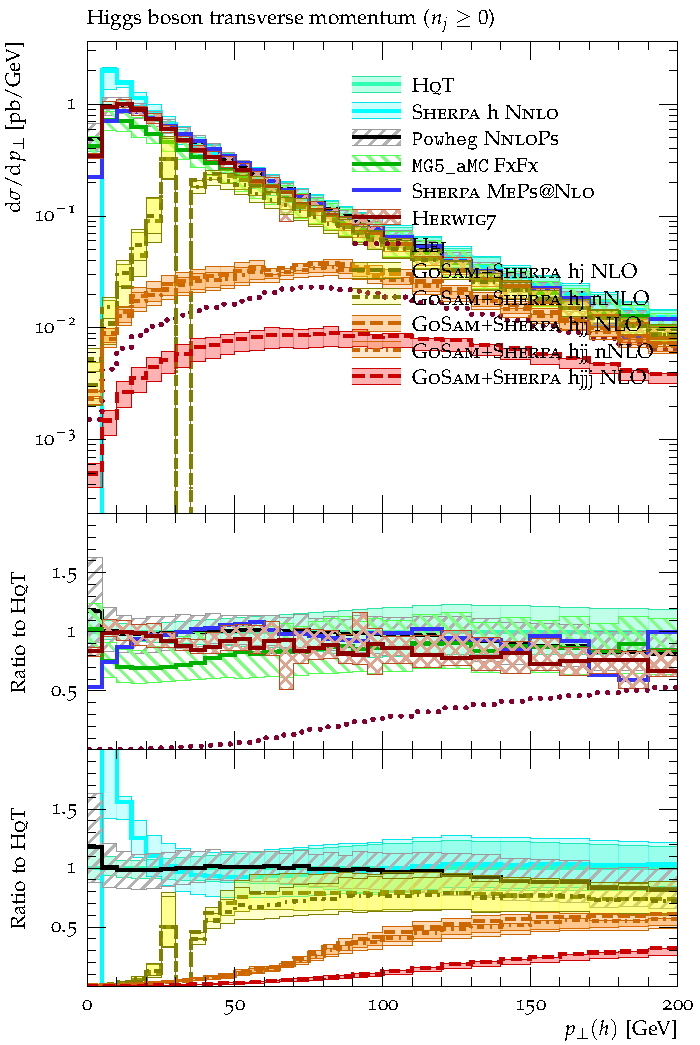
\includegraphics[width=0.47\textwidth]{figures/hjetscomp_H_pT_incl.pdf}
  \caption{\label{fig:hjetscomp:results:inclobs:hpt}%
    The Higgs boson transverse momentum in the inclusive event
    selection without (left) and with (right) uncertainties. For the
    ratios in the bottom panel, the same grouping strategy has been
    used as in Figure~\ref{fig:hjetscomp:results:inclobs:hy}, while
    the reference prediction has been changed from that of pure NNLO
    to the one as given by \HqT.}
\end{figure}

\begin{figure}[t!]
  \centering
  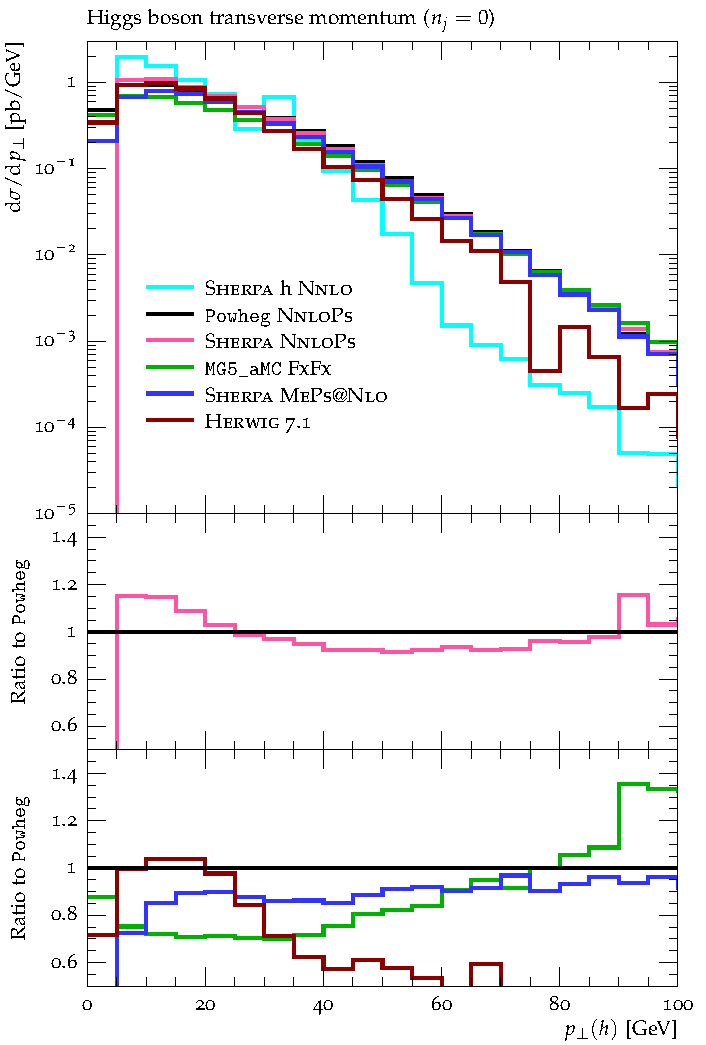
\includegraphics[width=0.47\textwidth]{figures/hjetscomp_u_H_pT_excl.pdf}
  \hfill
  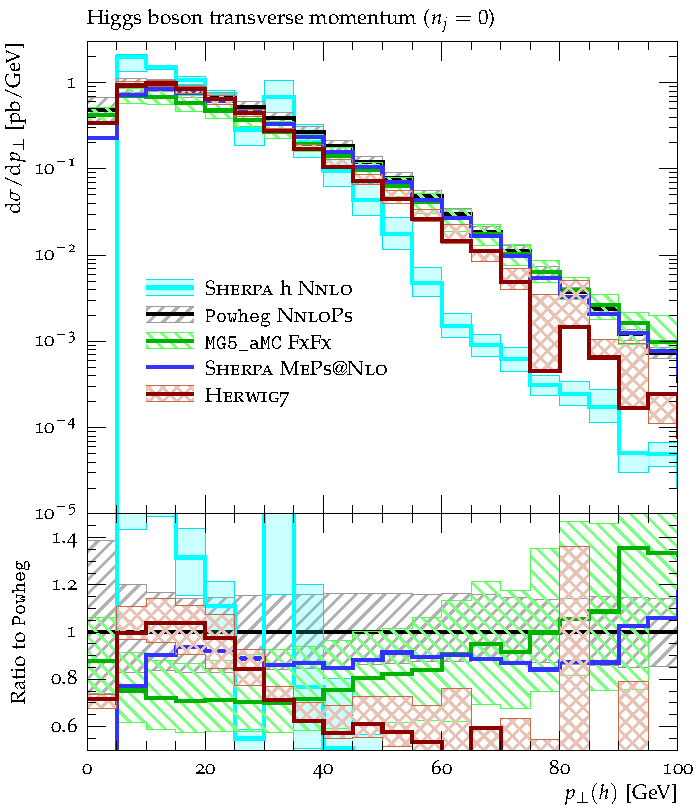
\includegraphics[width=0.47\textwidth]{figures/hjetscomp_H_pT_excl.pdf}
  \caption{\label{fig:hjetscomp:results:exclobs:hpt}%
    The Higgs boson transverse momentum in the exclusive event
    selection (i.e.~in the absence of any jet) without (left) and with
    (right) uncertainties. The bottom panel has been arranged as in
    the previous figure, apart from switching to a new reference curve
    which has been obtained from \Powheg \NNLOPS.}
\end{figure}

In Figures~\ref{fig:hjetscomp:results:inclobs:hpt} and
\ref{fig:hjetscomp:results:exclobs:hpt}, the inclusive and exclusive
(i.e.~vetoing jets above $30$\gev) Higgs boson transverse momentum
distributions are shown, respectively.  For the former, the ratios in
the bottom panel are taken with respect to the \HqT result, while
\Powheg \NNLOPS serves as the reference for the latter case. In
general, good agreement is found, with differences being somewhat more
pronounced in the exclusive case. For the inclusive version of the
$p_\perp(h)$ observable, the good agreement is observed with \HqT,
with some larger deviations evident at very low $p_\perp$. Here the 
resummation properties of the different parton showers dominate the 
spectra of the matched and merged predictions. While the
\Sherpa \NNLOPS curve starts about 15\% higher than both \HqT and \Powheg 
\NNLOPS at low $p_\perp$ it approaches the \HqT results at high $p_\perp$ 
in the fixed-order region. At the same time, \Powheg \NNLOPS follows 
\HqT closely up to scales of $\sim m_h$. Beyond that value, the 
dynamical scale employed \Powheg \NNLOPS accounts for the ensuing 
difference. The multi-jet merged calculations, due to their similar 
scale choices, follow the pattern of the \Powheg \NNLOPS prediction.
Note that the differences in \MGaMC's central scale
choice becomes less significant as the Higgs boson transverse momentum
increases. \Herwig clearly provides the softest spectrum and \Sherpa
as well as \MGaMC predict a noticeably different shape for the Sudakov
suppression at low $p_\perp$. This is not covered by the \HqT
uncertainty envelope. We refrain from showing any fixed order
prediction here because they are neither stable nor reliable at low
$p_\perp$ in the Sudakov region where resummation effects play a 
dominant role.

As shown in Figure~\ref{fig:hjetscomp:results:exclobs:hpt}, the
exclusive version of $p_\perp(h)$ exhibits deviations among the
predictions that become more sizable. The $p_\perp(h)$ distribution 
declines much faster, easily spanning three orders of magnitude 
between zero and $100$\gev. This observable is less straight forward 
than the inclusive $p_\perp$-spectrum as not only Sudakov effects 
dominate the low-$p_\perp$ region, but resummation effects are also 
entering through the veto on any jet activity. It thus necessitates 
both a proper description of small $p_\perp(h)$ region as well as 
jet production. Thus,
this is a stringent test of all predictions combining matrix elements and parton showers (ME+PS), as
the high transverse momentum of the Higgs boson is produced by a
combination of soft jets (those that are below the $30$\gev threshold)
and soft gluon radiation. Note that the comparison is now taken with respect to
\Powheg \NNLOPS. The inclusive 
NNLO calculation is shown to exemplify the failure of a fixed-order 
calculation on both accounts, and, thus, only the parton showered 
predictions are included in the study of the respective differences. 
Among them, apart from the differences already seen in the inclusive 
spectrum, both \NNLOPS calculations agree very well with one another, 
remaining within the 20\% uncertainty bands throughout the spectrum. 
While \Sherpa \MEPSatNLO remains mostly flat with respect to the \NNLOPS 
predictions, both \MGaMC and \Herwig exhibit difference in shape also 
also at larger transverse momenta. In the case
of \Herwig, they even grow larger than 40\%. 
From the resummation (i.e.~parton-shower)
point of view, all predictions are at the same level here, although
formally the \NNLOPS techniques lead to a more accurate description of
the exact zero-jet bin. The NLO merging approaches reduce to an \NLOPS
treatment in this zero-jet bin. It is however hard to infer this
formal difference from the behavior of the scale variation bands as
they are very comparable in size among all predictions. We conclude
that the deviation of the predictions probably provides us with a
better reflection of the true uncertainty.

\begin{figure}[t!]
  \centering
  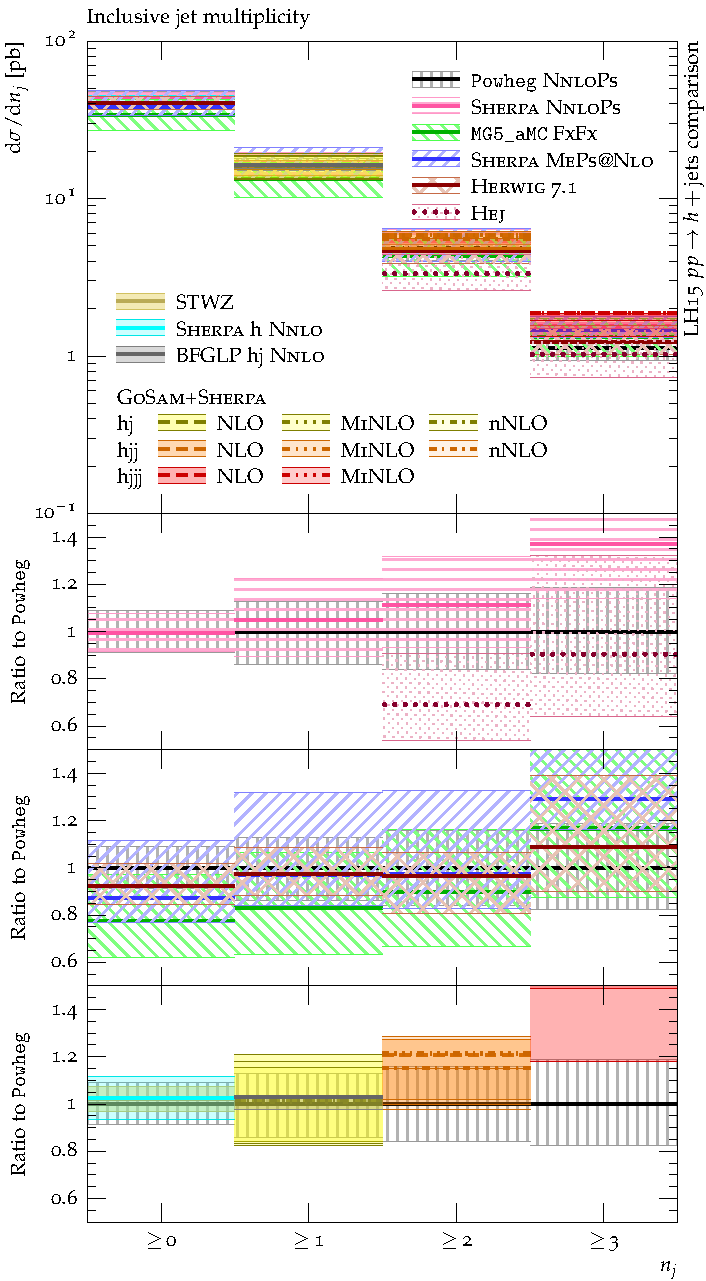
\includegraphics[width=0.47\textwidth]{figures/hjetscomp_NJet_incl_30.pdf}
  \hfill
  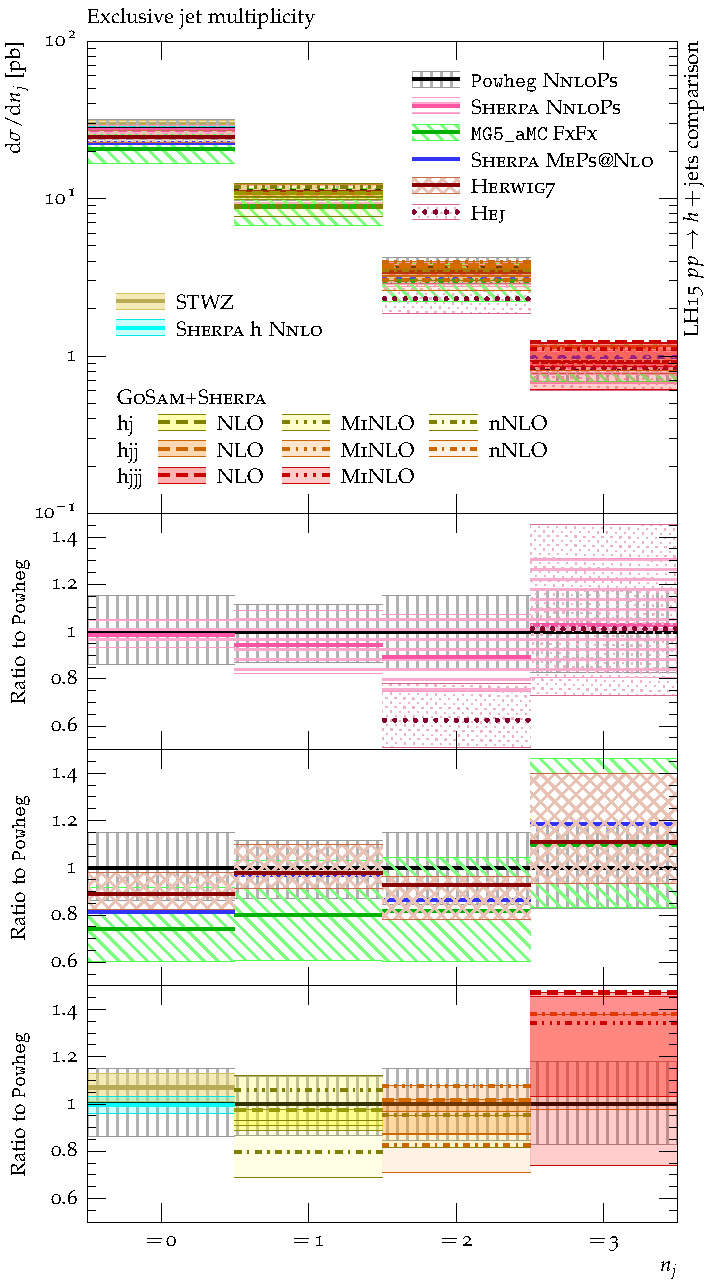
\includegraphics[width=0.47\textwidth]{figures/hjetscomp_NJet_excl_30.pdf}
  \caption{\label{fig:hjetscomp:results:inclobs:njets}%
    The inclusive (left) and exclusive (right) jet multiplicities
    including theoretical uncertainties as predicted by fixed-order
    calculations, resummed calculations, NNLO and NLO Monte Carlos. The
    bottom panel is divided up into three subplots all showing the
    ratios with respect to the \Powheg \NNLOPS prediction. The upper of these plots
    contains the \Hej and \Sherpa \NNLOPS ratios, while the middle one
    includes all NLO merged predictions (\MGaMC, \Herwig and \Sherpa)
    and the lower one shows all those listed in the bottom left legend
    of the main panel.}
\end{figure}

To obtain a first impression of how the different predictions 
compare beyond the zero-jet bins ($n_j\ge0$ and $n_j=0$) we 
look at the various inclusive and exclusive $n_j$ cross sections.
Accordingly, Figure~\ref{fig:hjetscomp:results:inclobs:njets} shows,
to the left, the inclusive ($n_j\ge N$) and, to the right, the
exclusive ($n_j=N$) jet multiplicity distributions up to $N=3$ 
using the previously defined \antikt jets with $p_\perp>30\gev$. Two
statements can be made before discussing the individual results in
more detail: first of all, the agreement between all results is
remarkable, and second, the details of the comparison are barely
altered when going from the inclusive description to the exclusive
description of the jet cross sections, apart from the obvious fact
that the exclusive jet bins always lie below the respective inclusive
jet bins. Although not shown here, when increasing the minimum jet-$p_\perp$ 
threshold to $50\gev$ the picture does not change significantly. 
Again, the bottom panels are split up into several ratio
plots with the common reference provided by the \Powheg \NNLOPS
results. The upper ratio plot depicts the \NNLOPS methods together
with \Hej, which only starts at $N=2$. Due to the scale choices in either 
\NNLOPS calculation they share a common inclusive cross section, with 
\Sherpa rising above \Powheg for higher jet multiplicities. Conversely,
\Hej undershoots by 30\% in the two-jet bin, where all predictions in this 
panel are LO accurate. In the three-jet bin, \Hej retains the LO accuracy 
while in both \NNLOPS calculations it is described by their respective 
parton showers only. Naturally, here the differences between the \NNLOPS 
predictions are largest. Please note, that the respective parton showering 
uncertainties are partially incorporated in the \Sherpa \NNLOPS uncertainty 
estimate while they are not assessed for \Powheg, resulting in a very flat 
uncertainty band. The central ratio plot confronts the NLO
matched and merged predictions with each other and against the common reference 
\Powheg \NNLOPS. All these predictions have claim NLO accuracy for $N=0,1,2$ 
and overlap well within uncertainties where the lower value for \MGaMC can 
again be attributed to the different scale choice. For $N=3$ only the \Sherpa 
\MEPSatNLO prediction retains its NLO accuracy while \MGaMC and \Herwig 
revert to LO, which is nicely reflected in the uncertainty estimates. 
Unsurprisingly, in the $N=3$ case, described by the reference with its 
parton shower only, all three NLO merged calculations predict larger 
cross sections.

Lastly, fixed-order predictions are shown for all jet multiplicities
at NLO (provided by \GoSam+\Sherpa) for the $1$-jet, $2$-jet and
$3$-jet bins and at approximate NNLO (labeled nNLO, provided by \Loopsim) 
for the $1$-jet and $2$-jet bins.
Complete NNLO predictions are shown for the 0-jet inclusive and
exclusive bins using \Sherpa without PS and for the 1-jet inclusive
bin using the prediction of Boughezal et al.~(BFGLP).
In addition, the zero-jet bin comparison
also contains the resummation prediction of Stewart et
al.~(STWZ) whereas the comparison for non-zero jet bins also
shows the \Minlo enhanced NLO calculations. All of the above are
grouped together in the lower ratio plot. For the zeroth bin, nice
agreement can be found between \Powheg and \Sherpa \NNLOPS as well as
the STWZ approach; the uncertainties also are of comparable
size. In the $1$-jet case, \Powheg (being NLO accurate in this bin)
resides 10\% above the pure NLO prediction, which simply is triggered
by the different scale choices. Unlike the inclusive Higgs boson
production case, the NNLO corrections for inclusive $1$-jet production
are small -- slightly negative for the central scale choice as given
in Eq.~(\ref{eq:bfglpScale}). There is a notable decrease in the scale
uncertainty with respect to the NLO band given by \GoSam+\Sherpa. The $2$-jet bin
shows the \GoSam NLO prediction just slightly above \Powheg, which
gives a LO prediction in this case. For the same reason, the \Powheg
uncertainties in the higher jet multiplicities are probably
underestimated. In the $3$-jet bin (both inclusive and exclusive), the
\GoSam+\Sherpa and \Sherpa \MEPSatNLO predictions clearly signal the absence of 
NLO corrections 
in the other predictions. The \Loopsim results for $h+j$ and
$h+jj$ are always somewhat below the respective \GoSam result
though the relatively large MC generation cut of $25$ \gev mean
the total rates predicted using \Loopsim should be interpreted with care.
Furthermore, compared to the NLO benchmark, the \Minlo approach
predicts 10-20\% larger cross sections for all non-zero jet bins.
Note that the \Minlo ratio for inclusive
$h+jjj$ turns out to be outside the plot range appearing at around
$1.65$ where the lower edge of the uncertainty band is seen kicking in
at a ratio value of $1.5$. In the cases where NNLO precision is available
the reduction in scale uncertainty is clear. For $n_j\geq1$ the variation around
$\mu_R=\sqrt{\Sigma_T}/2$ is about $5.5\%$ while for $n_j\geq0$ it is about $10\%$
around $\mu_R=m_h/2$. The latter result can be improved using the N${}^3$LO prediction
of Anastasiou et al. \cite{Anastasiou:2015ema} to only a few percent. In order to compare more
easily with results presented previously in the literature we give numerical values at NLO and NNLO
for different scale choices in Table \ref{tab:H1jXS}. As observed previously \cite{Boughezal:2015dra},
the convergence of the total cross-section is improved for scales that limit to $m_h/2$. The dynamical scale
of $\sqrt{\Sigma_T}$ defined in eq. \eqref{eq:bfglpScale} is slightly harder than the fixed scale given the
minimum jet $p_{T,j}>30$. On the other hand it is softer than $\hat{H}_T'$ defined in eq. \eqref{eq:hthatprime} which explains
the differences at NLO.

\begin{table}
  \centering
  \begin{tabular}{c||c|c|c}
    order \vphantom{$\int\limits_a^b$} & $\mu_R=\mu_F=\tfrac{1}{2}\,m_h$ & $\mu_R=\mu_F=\tfrac{1}{2}\,\hat{H}_T'$ & $\mu_R=\mu_F=\tfrac{1}{2}\,\sqrt{\vphantom{\big[}\Sigma_T}$ \\
    \hline\hline
    NLO \vphantom{$\int\limits_a^b$}  & $17.0^{+3.0}_{-2.9}$ pb & $13.5^{+2.0}_{-2.1}$ pb & $16.2^{+3.1}_{-2.8}$ pb \\\hline
    NNLO \vphantom{$\int\limits_a^b$} & -     & -     & $16.4^{+0.0}_{-0.9}$ pb \\
    \hline
  \end{tabular}
  \caption{
    The total cross-section for inclusive production of a Higgs boson and 
    one additional jet using different core scale choices.  The two 
    dynamical scales are $\hat{H}_T'=m_{T,h} + \sum_{\rm partons} p_T$ 
    (see also eq.~\eqref{eq:hthatprime}) and 
    $\Sigma_T = m_h^2 + \sum_{\rm jets} p_T^2$ 
    (see also eq.~\eqref{eq:bfglpScale}).
  }
  \label{tab:H1jXS}
\end{table}


\subsection{One-jet observables}
\label{sec:hjetscomp:results:1jobs}

In this section, we move away from the fully inclusive picture and
require the presence of at least one jet associated with the Higgs
boson. In some cases we also ask for the predictions where exactly one
jet is being resolved. Recall that the jets are defined based on the
anti-$k_T$ algorithm using $R=0.4$; they furthermore have to obey the
criteria that $p_\perp(j)>30\gev$ and $|\eta(j)|<4.4$. The set of
observables presented here includes the transverse momentum
distributions of the Higgs boson $h$, the leading jet $j_1$ and the
$hj_1$ two-body system as well as the rapidity spectrum of the leading
jet.

\begin{figure}[t!]
  \centering
  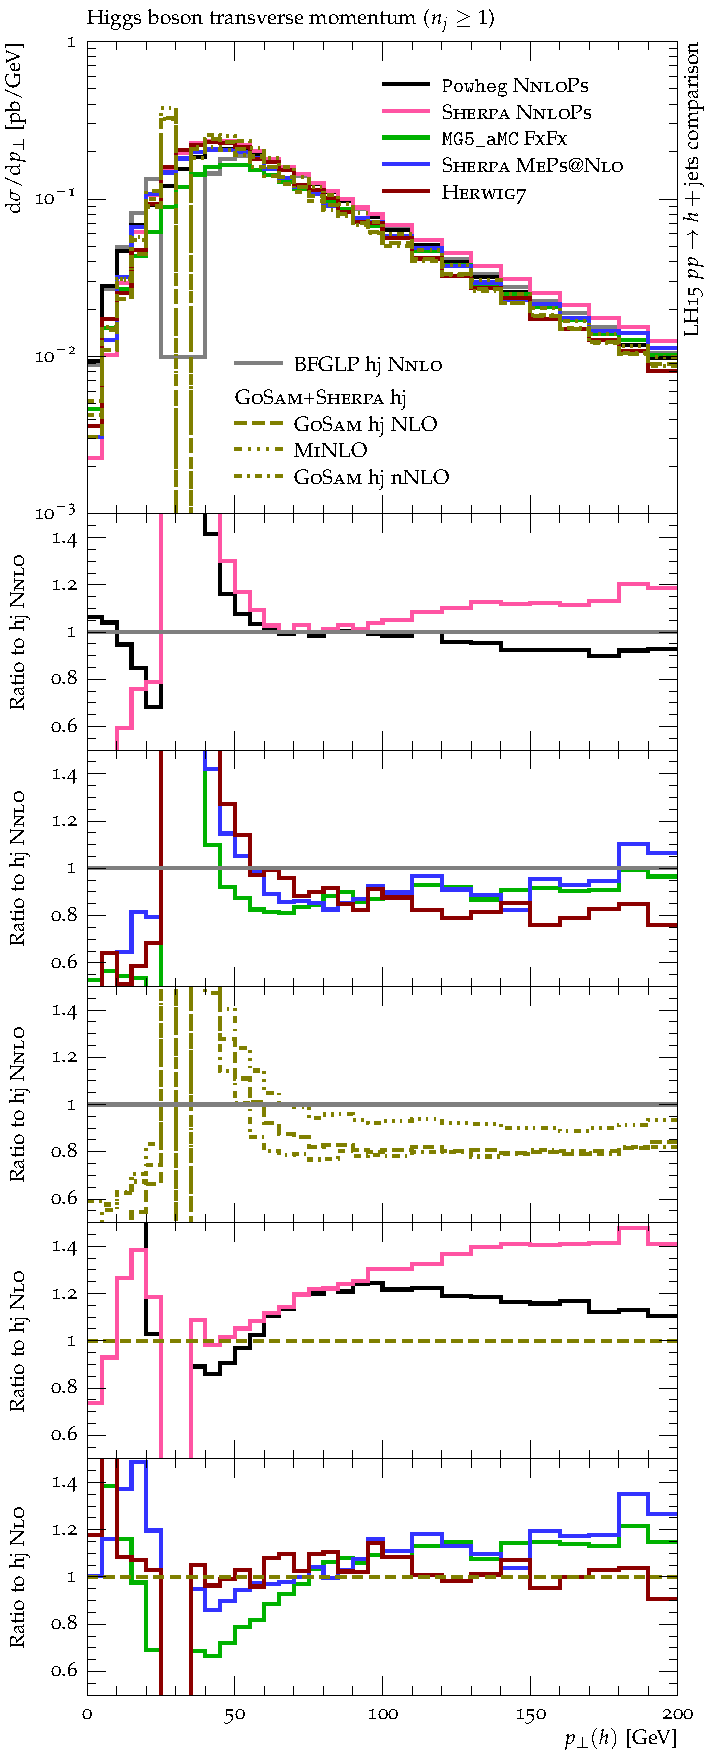
\includegraphics[width=0.47\textwidth]{figures/hjetscomp_u_H_j_pT_incl.pdf}
  \hfill
  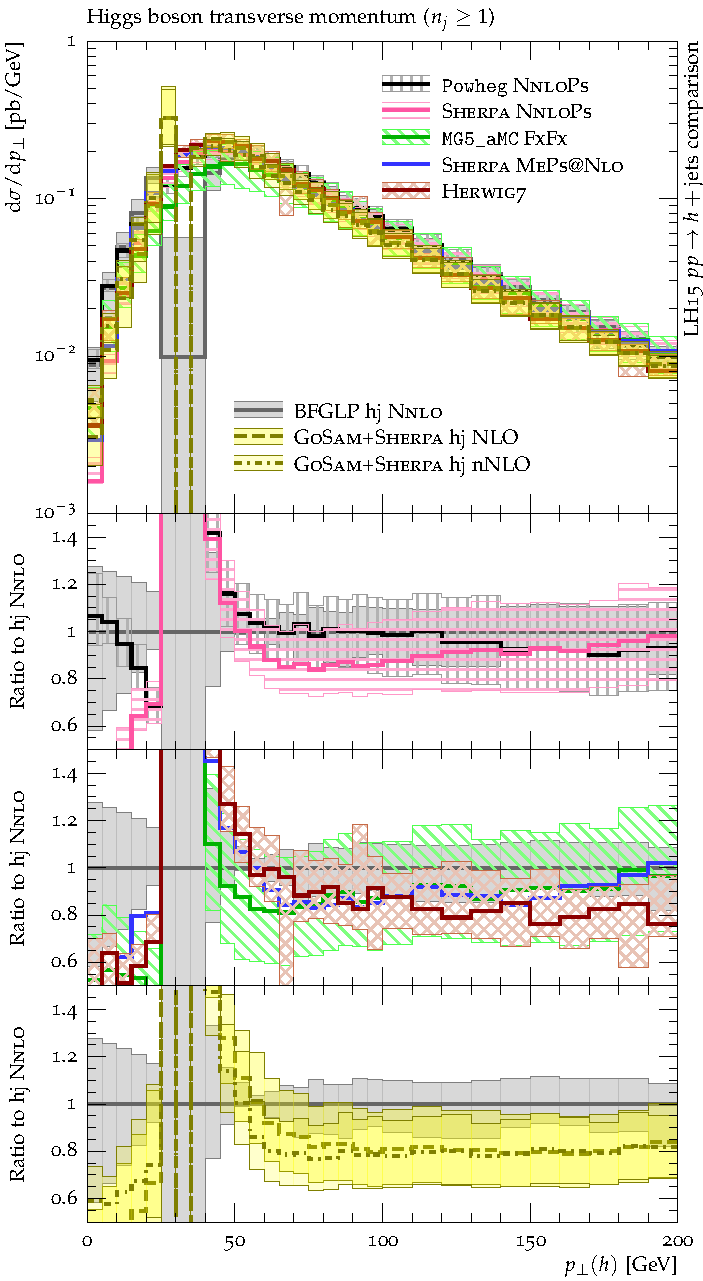
\includegraphics[width=0.47\textwidth]{figures/hjetscomp_H_j_pT_incl.pdf}
  \caption{\label{fig:hjetscomp:results:1obs:hpt}%
    The Higgs boson transverse momentum in the presence of at least
    one jet without (left) and with (right) uncertainty bands. The
    ratio plot panel is divided into five parts where the upper three
    exhibit the ratios wrt.~the \Powheg \NNLOPS result while the lower
    two show them wrt.~the NLO calculation for $h\pl1$~jet as
    provided by \GoSam+\Sherpa. The grouping in the ratio plots has
    been arranged to separately compare with each other the \NNLOPS
    predictions (first and fourth subplot), the NLO merging
    predictions (second and fifth subplot) and the fixed-order
    predictions (subplot in the middle).}
\end{figure}

\begin{figure}[t!]
  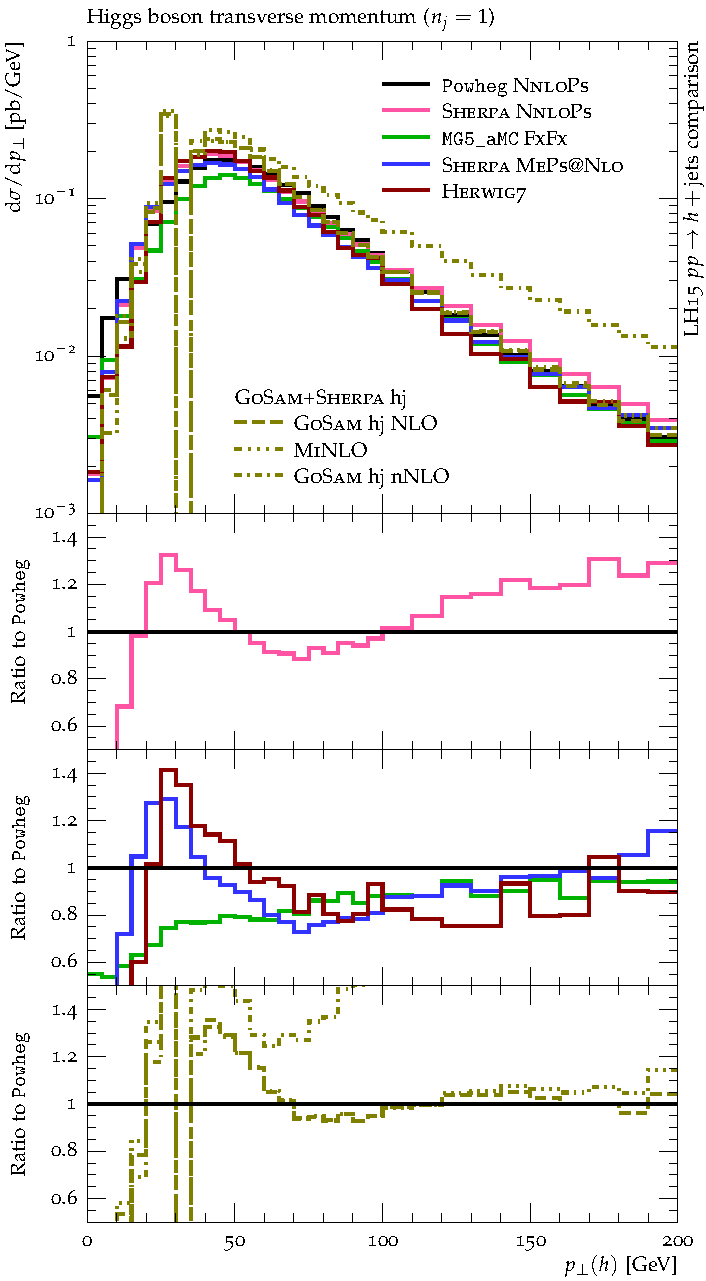
\includegraphics[width=0.47\textwidth]{figures/hjetscomp_u_H_j_pT_excl.pdf}
  \hfill
  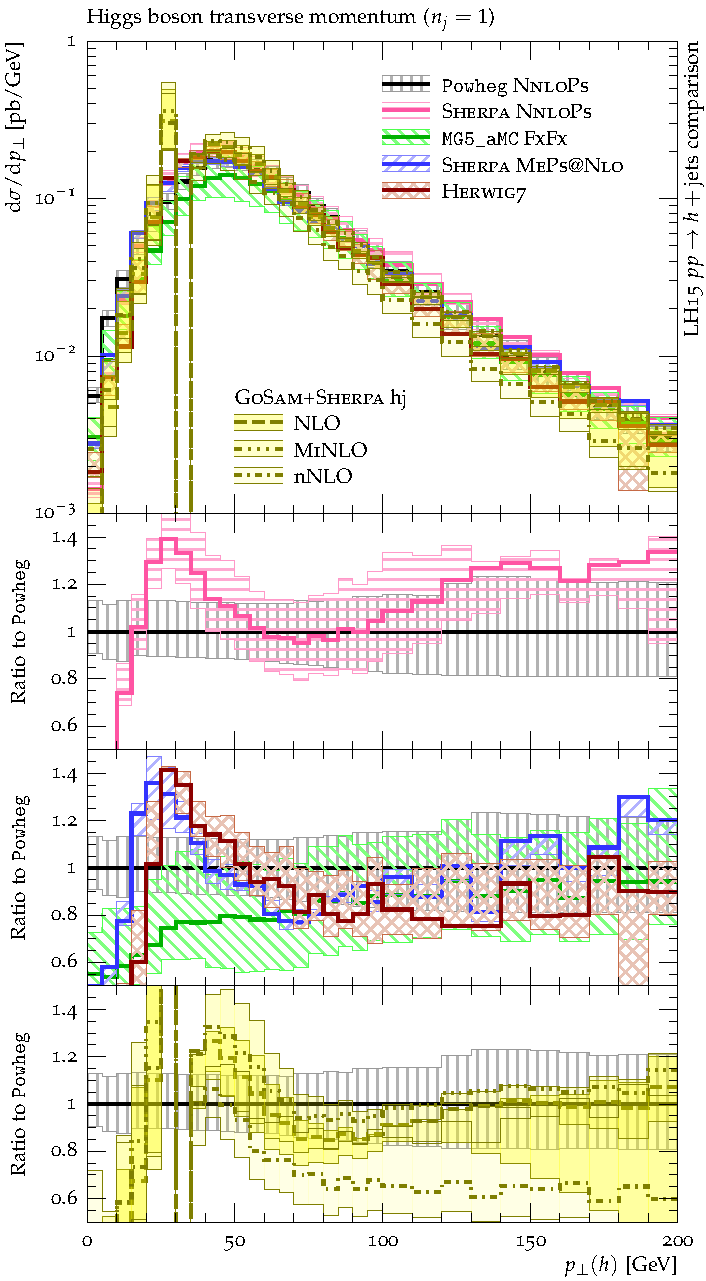
\includegraphics[width=0.47\textwidth]{figures/hjetscomp_H_j_pT_excl.pdf}
  \caption{\label{fig:hjetscomp:results:1obs:hpt_excl}%
    The Higgs boson transverse momentum in the presence of exactly one
    jet without (left) and with (right) uncertainty bands. The ratio
    plot panel is divided into three parts all of which depicting the
    corresponding ratios wrt.~the \Powheg \NNLOPS result. From top to
    bottom, the predictions are grouped such that the \NNLOPS results,
    the ME+PS results at NLO and the fixed-order results are compared
    directly in the first, second and third ratio plot, respectively.}
\end{figure}

The Higgs boson transverse momentum distribution in the presence of at
least one jet is shown in
Figure~\ref{fig:hjetscomp:results:1obs:hpt}. The exclusive version of
this plot, i.e.~where one requires the Higgs boson and the jet to be 
the only resolved final states present,
is presented in Figure~\ref{fig:hjetscomp:results:1obs:hpt_excl}.  As
for the zero-jet cases discussed earlier in
Figures~\ref{fig:hjetscomp:results:inclobs:hpt}~and~\ref{fig:hjetscomp:results:exclobs:hpt},
the one-jet $p_\perp(h)$ variables are prone to large, maybe sligthly
stronger, Sudakov effects that arise at low $p_\perp$ but also beyond
this area, in particular for the exclusive final states. Moreover, the
Sudakov shoulder effect can be observed for all fixed-order
predictions shown here. The jet-$p_\perp$ threshold leads to a
non-smooth behaviour of the $p_\perp(h)$ observable at LO, and
therefore to the existence of a critical point at $30\gev$ for which
the cancellations between real and virtual soft-gluon singularities
will be imperfect at any given fixed, higher order in perturbation
theory~\cite{Catani:1997xc}. For the BFGLP $hj$ NNLO  prediction, an
averaging procedure has been used to dampen the effect around the jet
threshold while for the NLO predictions, the large oscillations are a
clear indication of the instability emerging at the jet threshold.
Comparing the different fixed-order predictions, which are detailed in 
the third ratio plot, noticeable differences only
occur between the NNLO prediction and the four NLO predictions as
obtained from \Powheg and the three version of \GoSam+\Sherpa (pure
NLO, \Minlo and \Loopsim). The NNLO tail is harder by about 15\% which
is expected since the $p_\perp$ tail is affected by multi-jet
contributions. The NNLO treatment includes these contributions to a
larger extent, as it respectively includes $h\pl2$-jet and
$h\pl3$-jet contributions at the NLO and LO. For $p_\perp(h)< 30\,\gev$, 
the (N)NLO description is degraded to (N)LO. Here, the inclusion of 
the first term of the Sudakov resummation included in \Powheg benefits 
the BFGLP $hj$ NNLO calculation. However, it
can be noticed that apart from \Powheg and the BFGLP $hj$ NNLO
calculation all other approaches predict a more steeply falling
shoulder resulting in a significantly lower
cross section as $p_\perp(h)\to0$.
For larger $p_\perp(h)$ values, $p_\perp(h)>70\gev$, in general there
is good agreement between \Powheg, \MGaMC, \Sherpa and the NLO curves;
this can be expected as these predictions are all NLO-accurate. As
before, \Herwig tends to be softer, whereas \MGaMC using the nominal
$\tfrac{1}{2}m_h$ core scale turns out to be harder by almost 40\% as
inidcated by the upper edge of its corresponding uncertainty band, see
second or last subplot to the right in
Figure~\ref{fig:hjetscomp:results:1obs:hpt}. \Sherpa's \NNLOPS
prediction also features a harder tail than \Powheg owing to the
different scale setting procedures employed by the two approaches.
While in \Powheg the scale setting is accomplished through the \Minlo
procedure, \Sherpa's \NNLOPS uses the fixed scale choice of $\tfrac{1}{2}m_h$
and therefore enhances the $p_\perp$ tail with respect to the \Powheg's result. We
furthermore observe that apart from the BFGLP $hj$ NNLO computation, all
uncertainty envelopes are of similar size, which does not come as a
surprise because all of these predictions are effectively given at
NLO. The NNLO uncertainty band (shown in grey) is found to be
significantly smaller. Comparing the second and last ratio plots with
each other, we also notice that the ME+PS predictions are in better
overall agreement with the pure NLO prediction given by \GoSam{}+\Sherpa
than they are in agreement with \Powheg, with the exception of \MGaMC 
below $p_\perp(h)\lesssim \tfrac{1}{2}m_h$. This is surprising since all parton 
shower matched calculations are of the same intrinsic accuracy (NLO) and 
use similar local scale definitions along the lines of CKKW and include 
Sudakov factors of NLL accuracy. It may, however, be related to the way 
the resummation is controlled in \Powheg and the \MCatNLO-type matchings 
used in \MGaMC, \Herwig and \Sherpa. The different parton shower starting 
scales employed in \Herwig and \Sherpa ($\sim \tfrac{1}{2}m_h$), 
\MGaMC ($\sim m_h$) and \Powheg ($E_\text{CMS}$) do also play a role.

For the exclusive one-jet case, we reduce the number of ratio plots
and show only those that display the ratios to \Powheg in the same way
as before. Note that for the exclusive version of the observable, the
NNLO result is not available turning this comparison into one between
NLO-accurate predictions, except for the NNLO-approximate result given
by \Loopsim, labelled \GoSam $hj$ nNLO.
Figure~\ref{fig:hjetscomp:results:1obs:hpt_excl} clearly shows that
the differences among the results are very similar to those discussed
in the inclusive case; they are however pronounced such that the
deviations wrt.~the \Powheg \NNLOPS prediction for $h$ production
become larger for the full tranverse momentum range. There is one
exception to this: \Loopsim predicts a softer tail of the $p_\perp(h)$
distribution by about 20\%. This is easily understood as the tail of 
the exclusive distributions is made up of multiple soft emissions not 
captured by the \Loopsim approach.

\begin{figure}[t!]
  \centering
  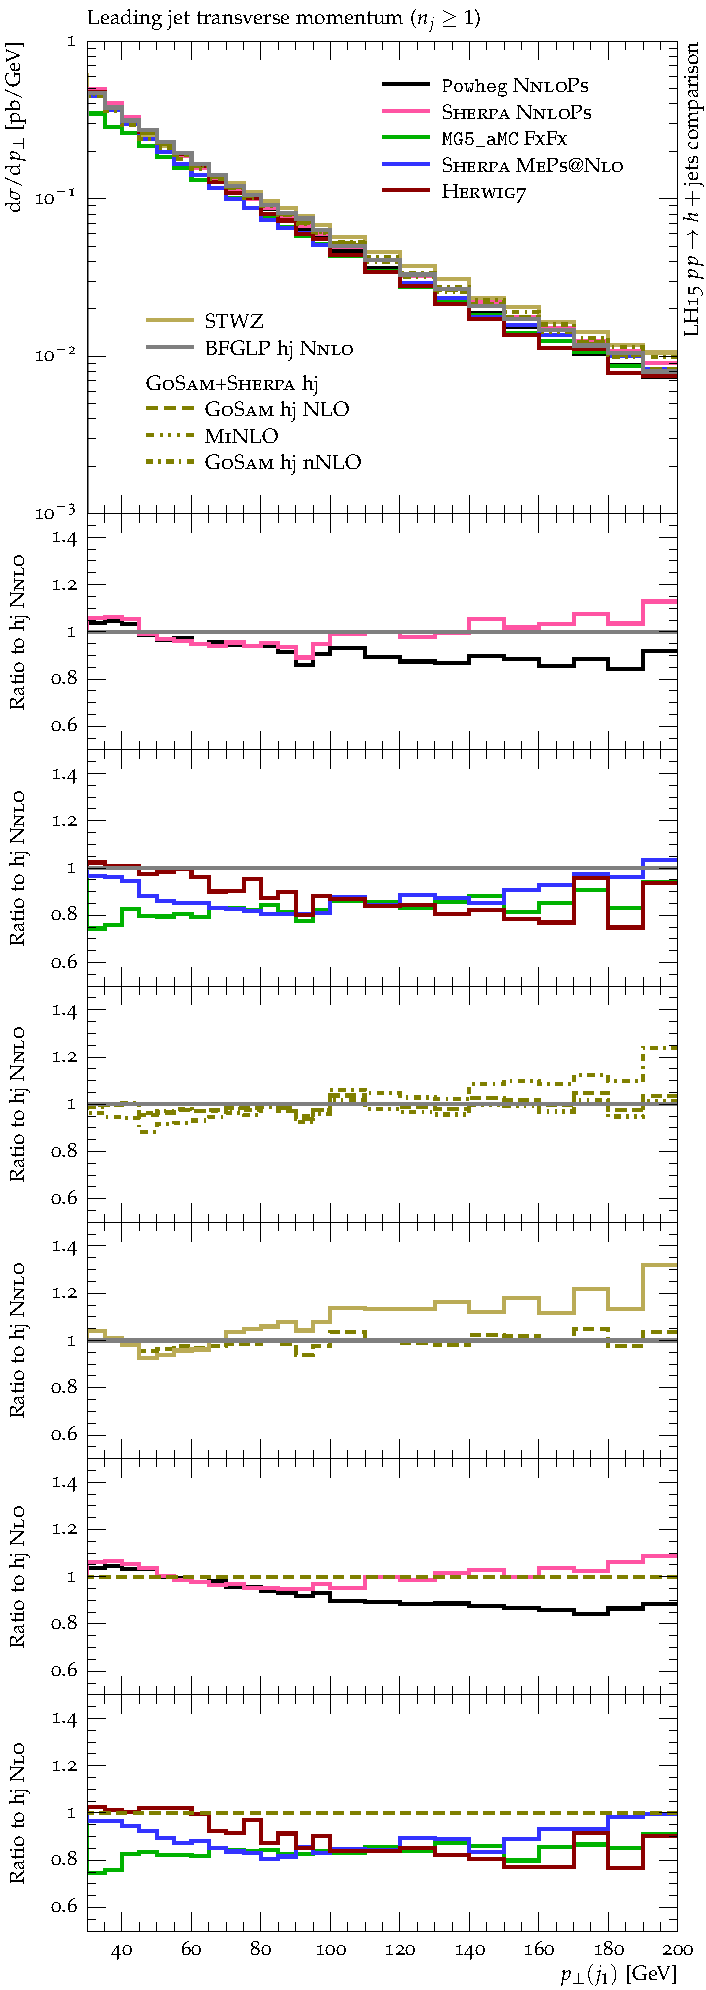
\includegraphics[width=0.47\textwidth]{figures/hjetscomp_u_jet1_pT_incl.pdf}
  \hfill
  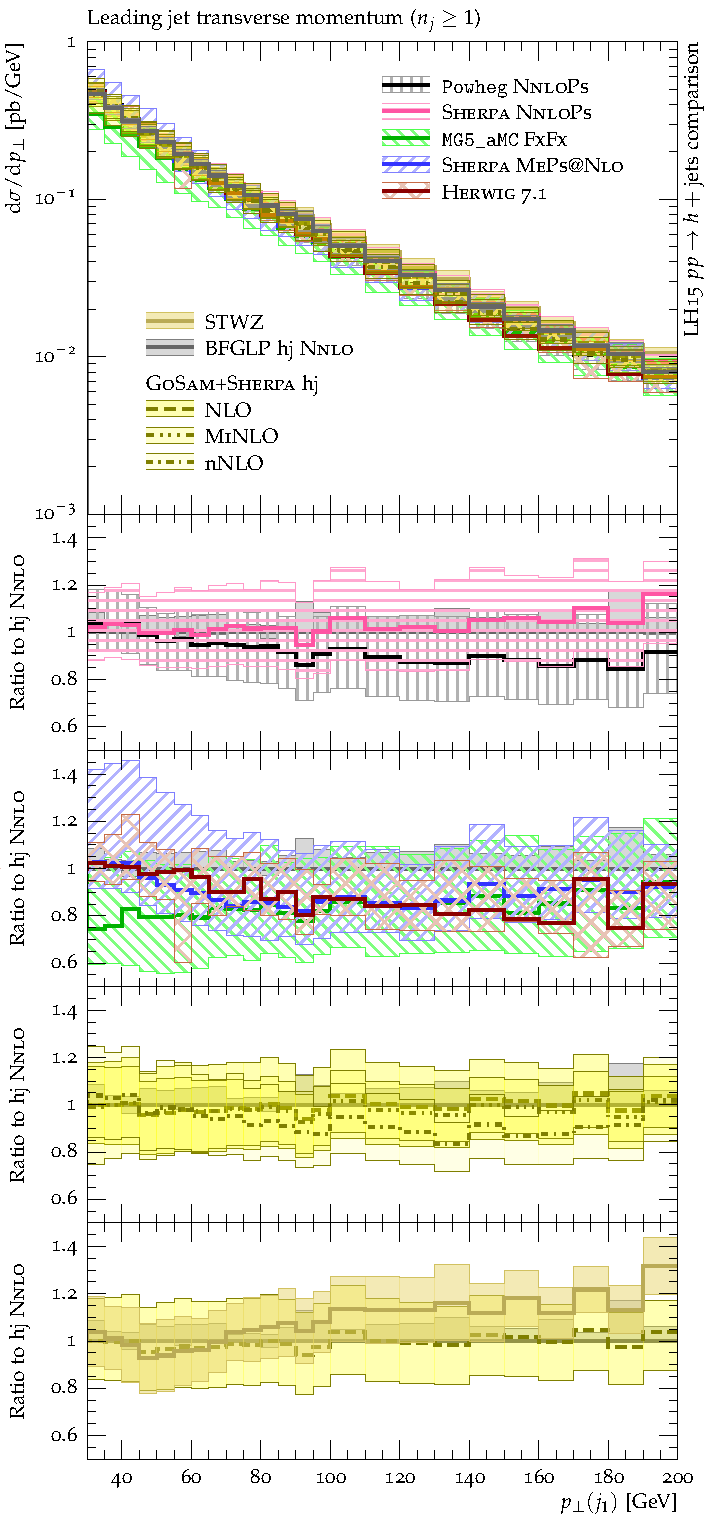
\includegraphics[width=0.47\textwidth]{figures/hjetscomp_jet1_pT_incl.pdf}
  \caption{\label{fig:hjetscomp:results:1obs:j1pt}%
    The leading jet transverse momentum distribution for
    $h\,+\!\ge\!\!1$-jet production, to the right (left) shown with
    (without) the uncertainty bands provided by the various
    calculations. The part below the main plot contains ratio plots
    taken wrt.~the NNLO result of the BFGLP group (subpanel one
    through four) and the NLO result given by \GoSam+\Sherpa (lowest
    two subpanels) following the same strategy for grouping the
    predictions as before (\NNLOPS versus NLO ME+PS versus fixed-order
    results). Note the layout of the first and last two subpanels is
    the same, apart from exchanging the reference.}
\end{figure}

\begin{figure}[t!]
  \centering
  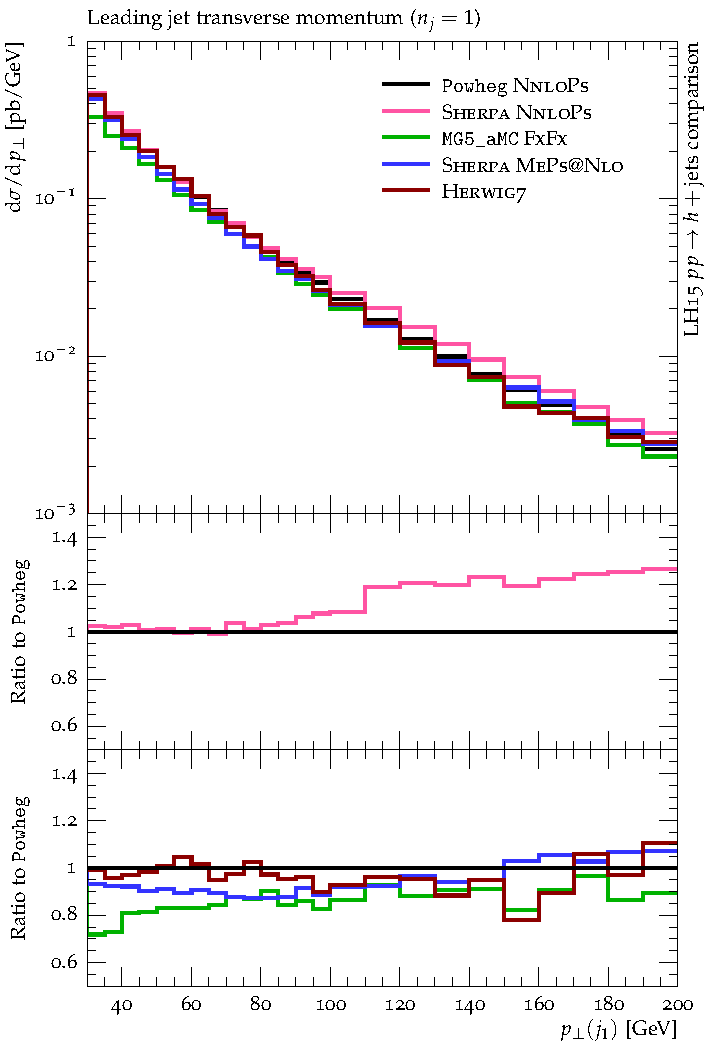
\includegraphics[width=0.47\textwidth]{figures/hjetscomp_u_jet1_pT_excl.pdf}
  \hfill
  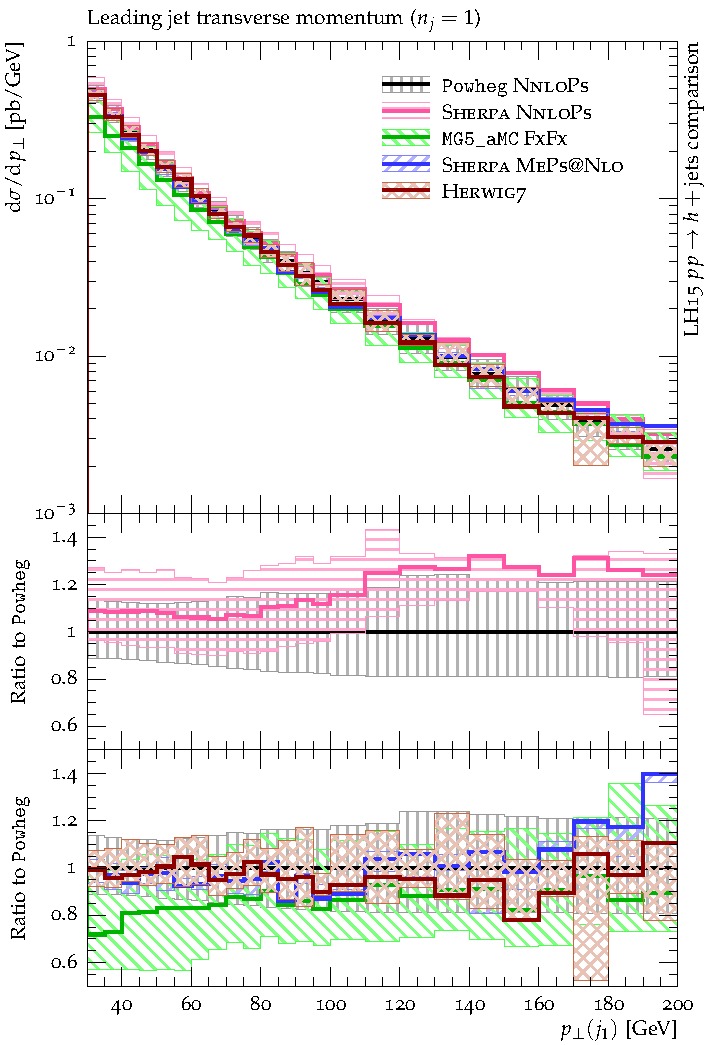
\includegraphics[width=0.47\textwidth]{figures/hjetscomp_jet1_pT_excl.pdf}
  \caption{\label{fig:hjetscomp:results:1obs:j1pt_excl}%
    The leading jet transverse momentum distribution for exclusive
    $h\pl1$-jet production, to the right (left) shown with (without)
    the uncertainty bands provided by the various calculations. Ratio
    plots are displayed in the lower part of the plot using the
    \Powheg \NNLOPS result for $h$ production as their reference.
    Predictions are grouped in similar fashion to the previous plots.}
\end{figure}

Next we discuss the leading jet transverse momentum distribution for
$h\,+\!\ge\!\!1$-jet final states. For this type of observable, we do not
expect large Sudakov effects (i.e. shifts owing to parton
showering/resummation). The impact of jet veto logarithms (owing to
the restriction that all jets be greater than $30\gev$) has been
examined and found to be reasonably small at NLO and
NNLO~\cite{Banfi:2012jm,Banfi:2015pju}. 
In the exclusive jet case, the $p_\perp(j_1)$ variable however is
prone to larger resummation effects, and we note that the scale
uncertainties shown will not reflect the true uncertainty. The
inclusive jet results for all approaches are shown in
Figure~\ref{fig:hjetscomp:results:1obs:j1pt} including the NNLO
prediction of the BFGLP group and the prediction of Stewart, Tackmann
et al. Figure~\ref{fig:hjetscomp:results:1obs:j1pt_excl} depicts the
exclusive one-jet case presenting the results obtained by the Monte
Carlo tools only; no fixed-order predictions are shown. Accordingly,
different reference predictions (NNLO and \Powheg) are used in the
ratio plots associated with
Figures~\ref{fig:hjetscomp:results:1obs:j1pt} and
\ref{fig:hjetscomp:results:1obs:j1pt_excl}. 
Overall we find a rather remarkable agreement
between all results where the largest deviations rarely exceed the
20\% mark. For the exclusive lead-jet transverse momentum distribution
of Figure~\ref{fig:hjetscomp:results:1obs:j1pt_excl}, this means that
all predictions are in reasonably good agreement with \Powheg. The
\MGaMC prediction is lower than \Powheg for basically the entire
transverse momentum range, again because of the central scale choice
being higher than in the other approaches. For the inclusive lead-jet
transverse momentum spectrum (see
Figure~\ref{fig:hjetscomp:results:1obs:j1pt}), the remarkable
agreement implies that all predictions indeed lie within each other's
uncertainty bands. The quoted uncertainties are similar in size, with
values at and around the 20\% level, and only those of the BFGLP $hj$ NNLO
calculation are significantly smaller. 

Despite the good agreement seen among all predictions in
Figure~\ref{fig:hjetscomp:results:1obs:j1pt}, it is worthwhile to go
through the ratio plots and discuss some of the interesting features.
In the top ratio panel, the two \NNLOPS predictions are compared to the
NNLO $h\,+\!\ge\!\!1$-jet prediction. The agreement among all three is
good at low transverse momentum, but at higher $p_\perp(j_1)$ there is
a tendency for \Sherpa \NNLOPS to move to the upper edge of the NNLO 
uncertainty band and \Powheg \NNLOPS to move slightly below, resulting 
in a 20\% net difference between the two. Again, this is a result of using
$\mu=\tfrac{1}{2}m_h$ within \Sherpa versus using \Minlo/CKKW scales within the
\Powheg approach. In the second ratio panel, \Herwig, \Sherpa and \MGaMC
(taking into account its larger limit scale) agree reasonably well
with each other over the entire transverse momentum range, but fall
about 15\% low wrt.~the BFGLP prediction in the mid-range of the
$p_\perp$ distribution. The third ratio panel shows that there is almost no
difference in normalization nor shape between the NNLO and the NLO
$h\,+\!\ge\!\!1$-jet predictions using the given scale choice,
cf.~Eq.~(\ref{eq:bfglpScale}). This extends to the \Minlo reweighted
NLO result and the nNLO prediction provided by the \Loopsim approach, although the
latter is somewhat softer. In the bottom ratio panel, the STWZ prediction, 
constituting a resummation improved NLO calculation for this observable,  
agrees with the NNLO prediction at low $p_\perp$, but rises up to 30\%
higher at the largest $p_\perp$ values, mainly due to its fixed scale choice. 

In summary, the fixed-order NNLO prediction of the BFGLP group, which
has the best theoretical uncertainties available, is in good agreement
with the \Sherpa \NNLOPS prediction, and to a
somewhat lesser extent, with the \Powheg \NNLOPS predictions. The level of
moderate disagreements observed with the multijet merged calculations 
may be due to the somewhat different scale choices that are still important 
at NLO. The largest deviation seen with \MGaMC is can mainly be traced to 
its different choice of central scales. There is no sign of any serious 
impact of the merging of the
fixed-order predictions with parton showers, as expected for such an
inclusive cross section.

\begin{figure}[t!]
  \centering
  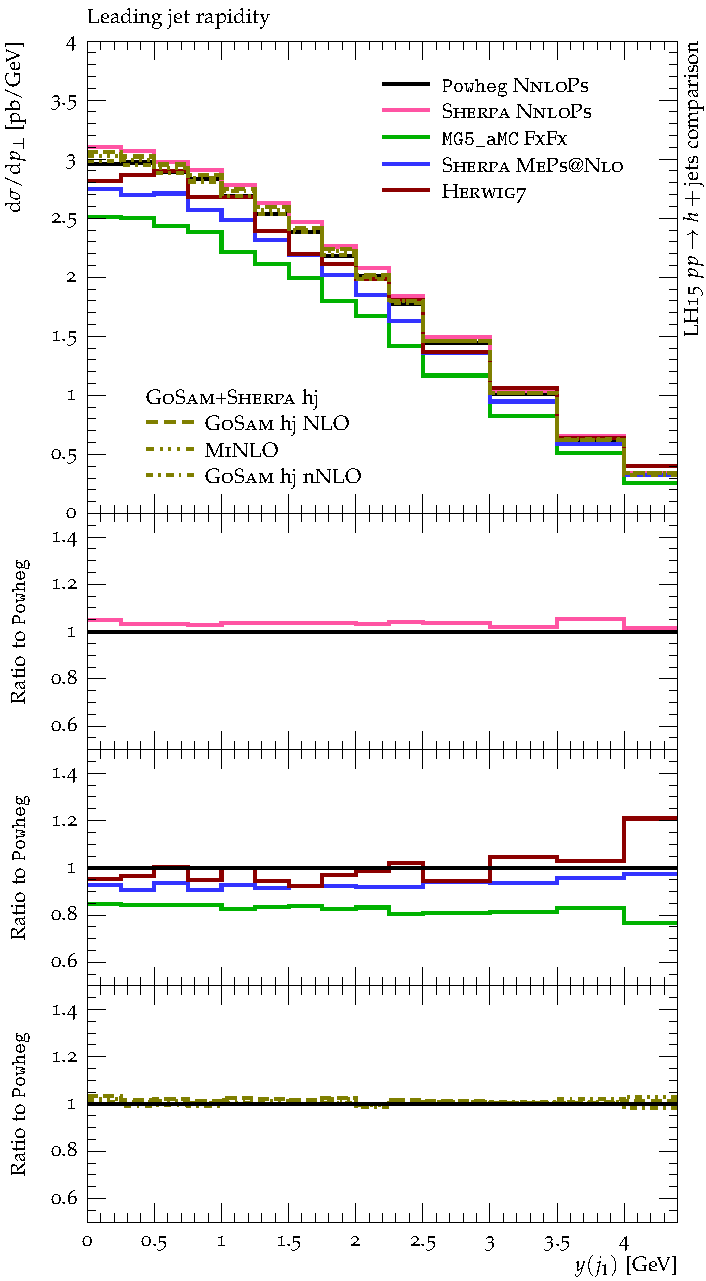
\includegraphics[width=0.47\textwidth]{figures/hjetscomp_u_jet1_y.pdf}
  \hfill
  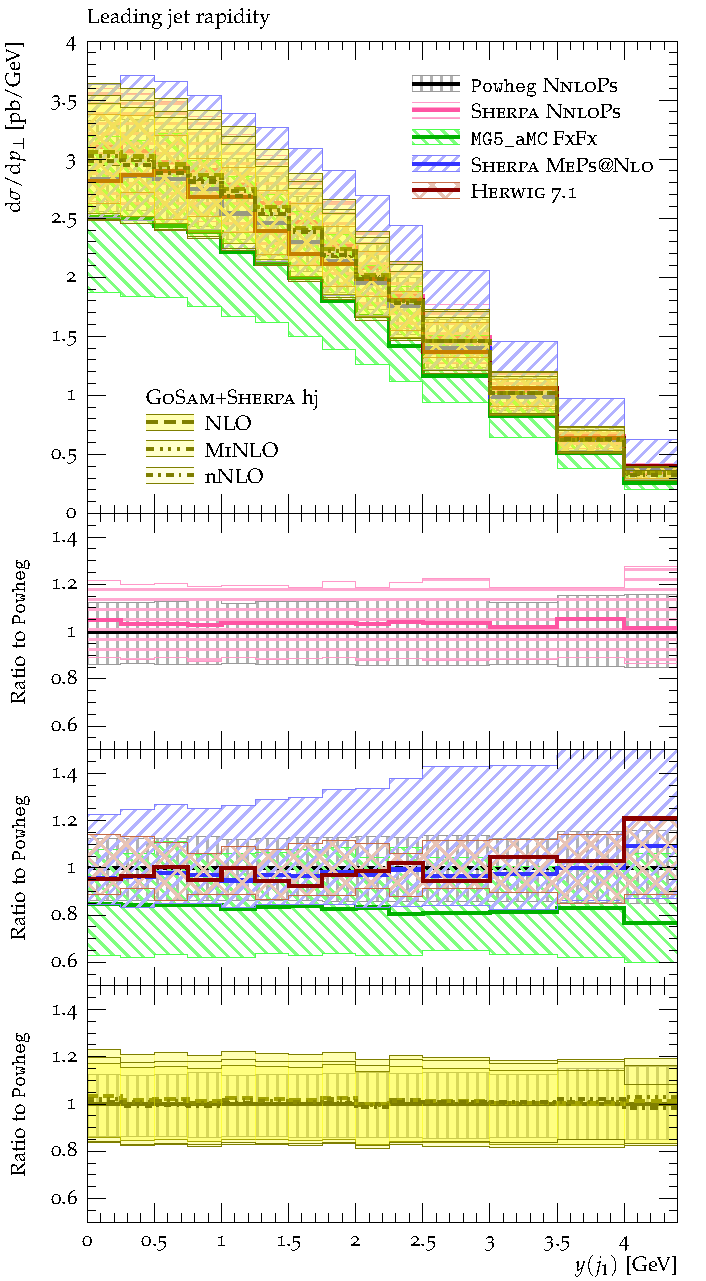
\includegraphics[width=0.47\textwidth]{figures/hjetscomp_jet1_y.pdf}
  \caption{\label{fig:hjetscomp:results:1obs:j1y}%
    The rapidity distribution for the leading jet in $h\,+\!\ge\!\!1$-jet
    production, shown without (left) and with (right) theoretical
    uncertainties. Ratio plots are displayed in the lower part of the
    plot using the \Powheg \NNLOPS result for $h$ production as their
    reference. Predictions are grouped, from top to bottom, according
    to the categories \NNLOPS, ME+PS at NLO and NLO fixed order.}
\end{figure}

\Todo{MS: Too colloquial?}

Did we talk about great agreement in the previous case where we
discussed the $p_\perp(j_1)$ distribution, the agreement found for the
rapidity distribution of the lead jet, $y(j_1)$, is magnificient, as
demonstrated by Figure~\ref{fig:hjetscomp:results:1obs:j1y}. We were
to expect that due to the consistency of the $p_\perp(j_1)$ predictions and earlier findings
concerning $y(h)$, see Figure~\ref{fig:hjetscomp:results:inclobs:hy}.
We basically do not observe any shape differences, and the rate
differences follow the already established pattern where most
noticeably the \MGaMC cross section is reduced owing to their choice
of using a higher central scale. Again, uncertainty envelopes are
by and large similar in size and do not point to any shape changes
when varying the scales; \Herwig's band is slightly narrower while
\Sherpa \MEPSatNLO's and \MGaMC's band are somewhat wider compared 
to all other NLO-accurate predictions.

\begin{figure}[t!]
  \centering
  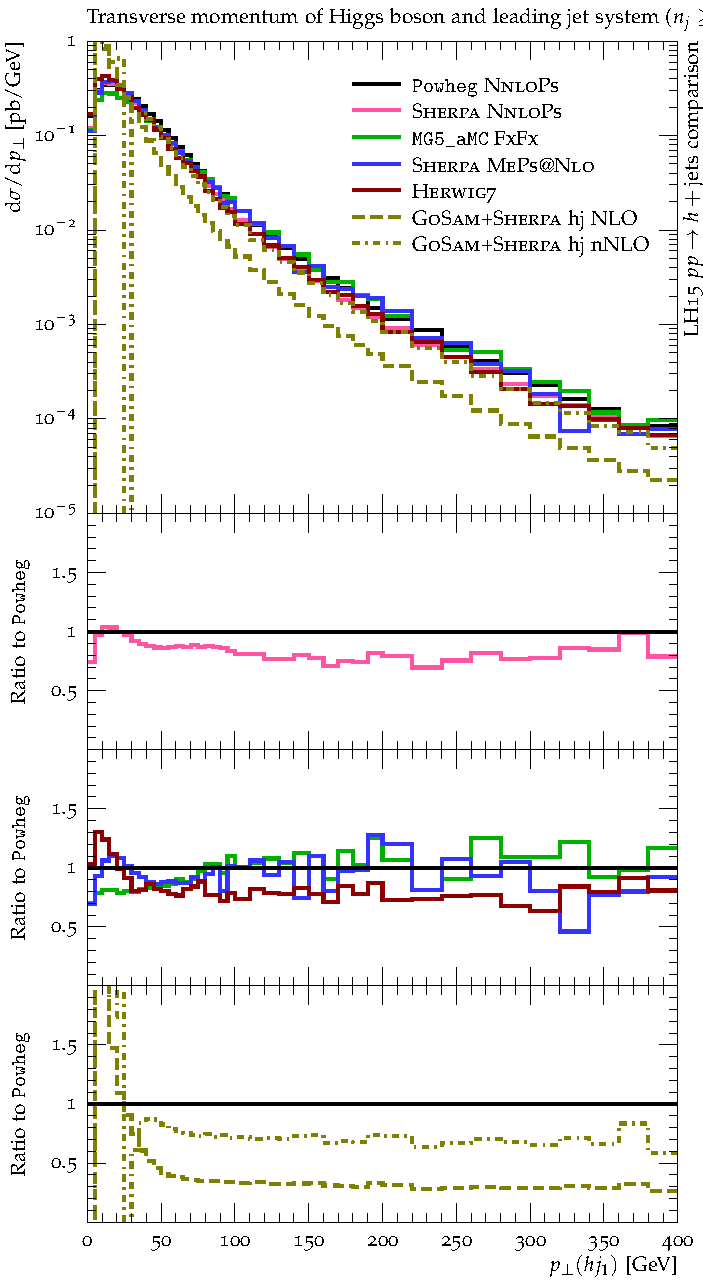
\includegraphics[width=0.47\textwidth]{figures/hjetscomp_u_Hj_pT_incl.pdf}
  \hfill
  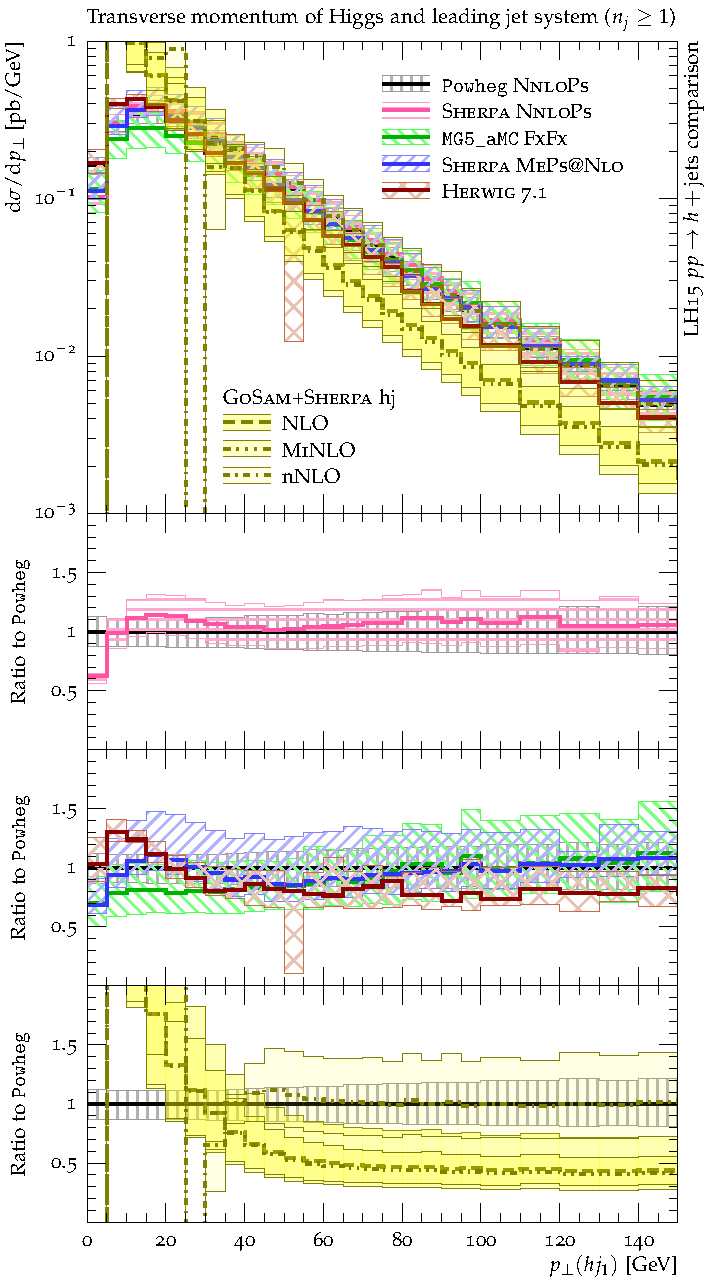
\includegraphics[width=0.47\textwidth]{figures/hjetscomp_Hj_pT_incl.pdf}
  \caption{\label{fig:hjetscomp:results:1obs:hj_pt}%
    The transverse momentum of the Higgs-boson-leading-jet system in
    the presence of at least one jet. For better visibility, results
    are shown without (left) and with (right) theoretical
    uncertainties. The plot layout exactly corresponds to that of
    Figure~\ref{fig:hjetscomp:results:1obs:j1y}, except for the
    extended $\hat y$-axis range in the ratio plots.}
\end{figure}

\begin{figure}[t!]
  \centering
  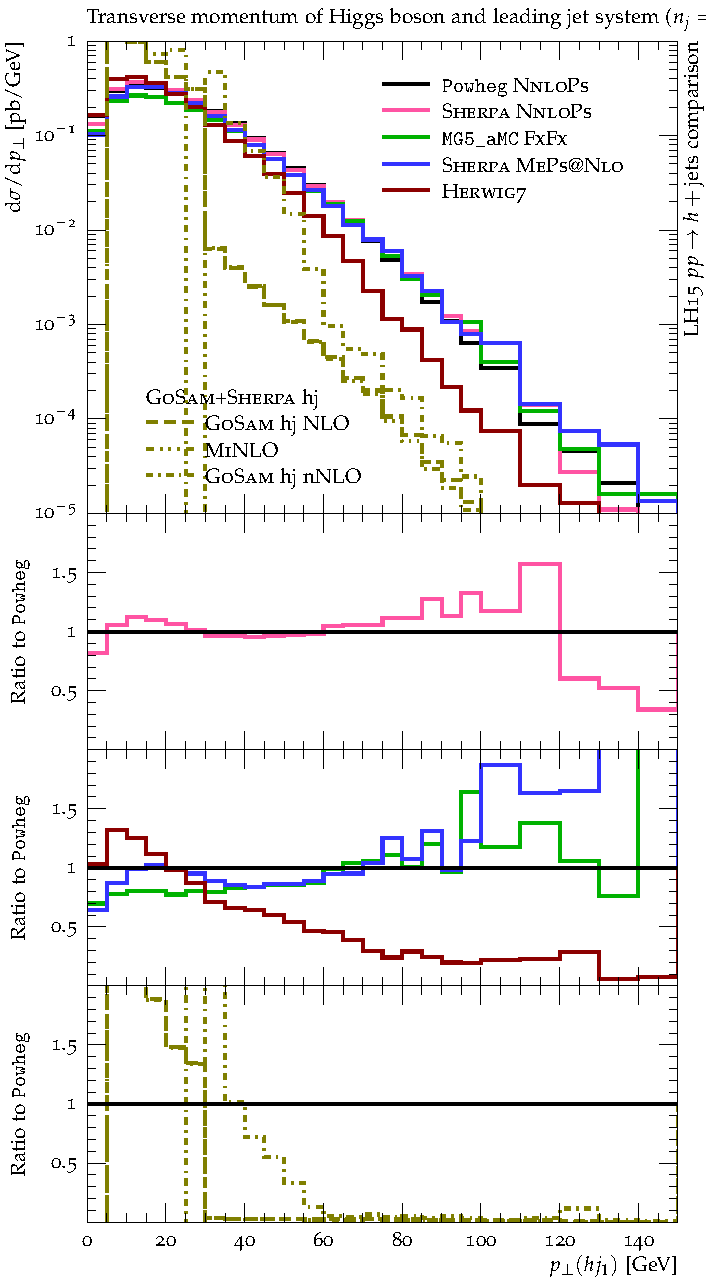
\includegraphics[width=0.47\textwidth]{figures/hjetscomp_u_Hj_pT_excl.pdf}
  \hfill
  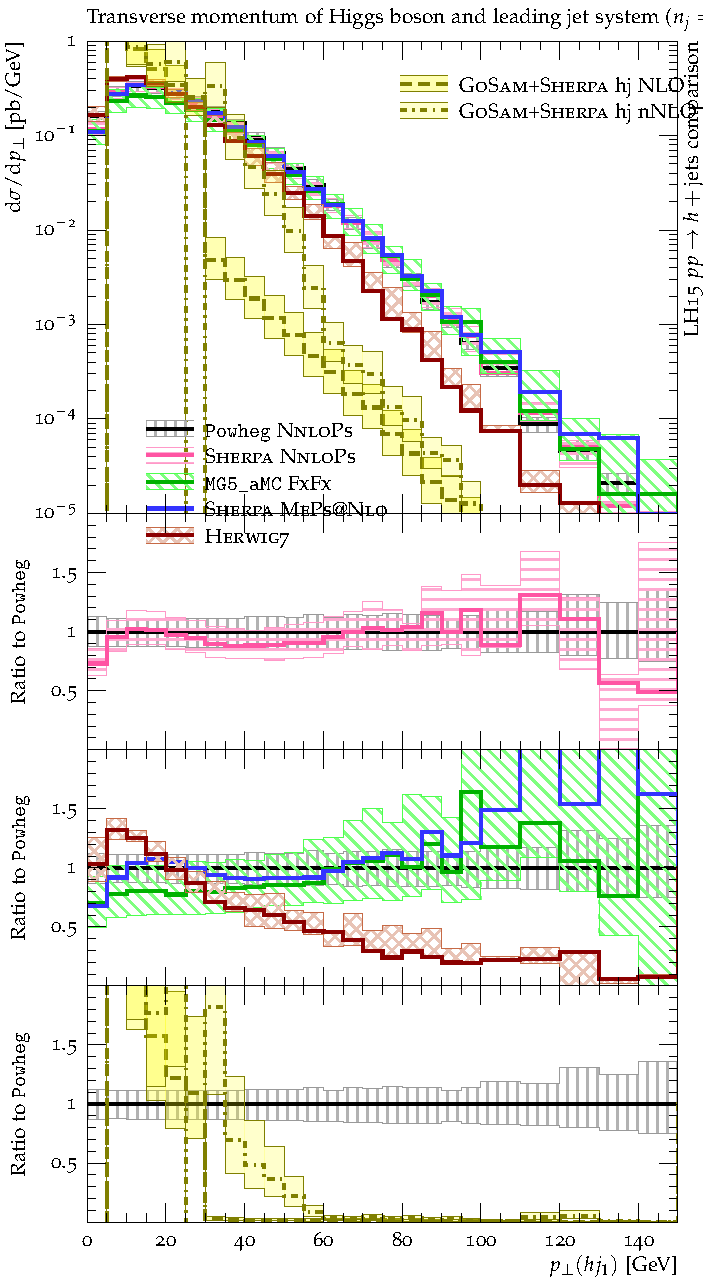
\includegraphics[width=0.47\textwidth]{figures/hjetscomp_Hj_pT_excl.pdf}
  \caption{\label{fig:hjetscomp:results:1obs:hj_pt_excl}%
    The transverse momentum of the Higgs-boson-leading-jet system in
    the presence of exactly one jet. Again, results are shown without
    (left) and with (right) theoretical uncertainties as given by the
    different groups. Note that the plot layout corresponds exactly to
    that of Figure~\ref{fig:hjetscomp:results:1obs:j1y}, except for
    the extended $\hat y$-axis range used in the ratio plots.}
\end{figure}

We finish this section by examining the results for the transverse
momentum of the Higgs-boson plus leading-jet system. In other words,
we are interested in studying the different answers in describing the
recoil of the $hj_1$ system. In the inclusive one-jet case depicted in
Figure~\ref{fig:hjetscomp:results:1obs:hj_pt}, the system may recoil
against a second jet (or secondary jets) plus soft radiation, while
for the exclusive jet scenario shown in
Figure~\ref{fig:hjetscomp:results:1obs:hj_pt_excl}, it is only soft
radiation that recoils against the $hj_1$ system. The latter case will
therefore be strongly affected by the level at which resummation is
taken into account. Formally, for the observable in question, the
predictions of highest accuracy are facilitated by the NLO merging
approaches as they provide an NLO description of the second jet; all
other predictions are only LO accurate in the second jet, i.e.~larger
differences can be expected. In the exclusive ($=1$-jet) case, all
predictions that include parton showering operate at the same level of
precision while the fixed-order calculations cannot do anything but
fail in describing the $p_\perp(hj_1)$ distribution.

For the $h\pl\ge1$-jet events, differences of $\mathcal{O}(30\%)$ are
observed among the ME+PS predictions below the jet threshold, while
there is better agreement at higher $p_\perp$ values, where again
\Herwig turns out to be on the softer side. The \Powheg and \Sherpa \NNLOPS 
curves surprisingly fit right in with the ME+PS results throughout 
the spectrum. The mostly comparable
behaviour of the \NNLOPS results to those obtained from NLO merging is
not what one would expect a priori, however the NNLO matching seems to
constrain the parton showers in a beneficial way (via sophisticated
choices for setting the renormalization, factorization and resummation
scales) such that the LO+PS treatment of the $h\,+\!\ge\!2$-jet rate
obtains a more appropriate normalization. The $hj$ NLO calculations
(i.e.~the pure and \Minlo reweighted \GoSam{}+\Sherpa results) cannot
compete with this performance since they miss an adaquate description 
of the second jet giving recoil to the $hj$-system.
Correspondingly, the $p_\perp(hj_1)$ observable is described poorly
with values clearly overshooting below the jet threshold due to the
missing Sudakov suppression and undershooting by 60\% beyond
$p_\perp=50\gev$ due to missing higher (than two-) jet multiplicity
contributions. It is interesting to see that the \Loopsim procedure
lifts this large discrepancy in the $p_\perp$ tail, concluding that 
an adequate description of a second and third jet is sufficient to 
describe this observable in this regime. Thus, the good agreement
with the ME+PS results is largely driven by the $hjj$ NLO component
used to build the nNLO prediction for the $h\,+\!\ge\!\!1$-jet
process. However, as a result of the cut-off dependence of the
procedure nothing can be said about the $p_\perp<25\gev$ region.
Lastly, we comment on the uncertainties quoted by the different
calculations: the \GoSam, \Minlo and \Loopsim envelopes have an
appropriate size reflecting the underlying LO nature of the
$p_\perp(hj_1)$ prediction above the jet threshold. \MGaMC and \Sherpa
\MEPSatNLO on the one side and \Herwig on the other side produce NLO
variations that are fairly different in size. However, the \Herwig as
well as the \Powheg envelopes are most likely underestimated, in
particular the \Powheg band does not behave as expected from a LO
variation for above-jet-threshold $p_\perp$. The \Sherpa \NNLOPS bands
here are somewhat larger than those of \Powheg but still do not 
reflect the LO nature of the prediction.

The exclusive (exactly one jet) case in describing the $p_\perp(hj_1)$
observable is shown in Figure~\ref{fig:hjetscomp:results:1obs:hj_pt_excl}.
Apart from the \NNLOPS outcomes, there is a much greater divergence of
the predictions for exactly one jet, especially at high $p_\perp$.
Recall this time, the recoil is generated only from soft emissions, and
it is clear that a highly exclusive distribution such as the one in
question serves as a stress test for the ME+PS as well as the \NNLOPS
predictions (in fact any parton shower or resummed prediction). For
the same reason, caution has to be taken in interpreting the shown
uncertainties. The current case is similar to the case for the Higgs
boson $p_\perp$ distribution with no jets and it is no surprise that
different approaches can lead to different answers. Most notably, we
observe \NNLOPS predictions that are in slightly worse agreement as
compared to the inclusive case, the expected complete failure of the
\GoSam{}+\Sherpa results (including the \Loopsim result where the
one-jet requirement obliterates the effect that yielded the
improvement in the inclusive case),%
\footnote{Owing to the kinematic constraints on the jets, harder
  radiation that goes forward does not get identified as a jet;
  these contributions actually form the (naively unexpected)
  $p_\perp>30\gev$ tail of the \GoSam results though the mechanism is
  highly suppressed.}
and the severe decline of the \Herwig differential cross section
dropping to about 25\% wrt.~the \Powheg result at $p_\perp\sim100\gev$.

\Todo{the pT plot range of the hj1 sytem goes out to 400, in the pT
  observables before we mainly did do 200? Any opinions? pro: it's a
  system pT; contra: mainly LO, all others are 200.}



\subsection{Dijet observables}
\label{sec:hjetscomp:results:2jobs}

\Todo{similarly to previous todo: plot range of hj1j2 system goes out
  to 400, but here also for pThiggs,
  fig~\ref{fig:hjetscomp:results:2obs:hpt_j2pt}, for the latter at
  least we should go to 200 as in the other pThiggs plots}

\Todo{single-particle rapidity plots, yHiggs, yJet1, in paper have a
  [GeV] legend ... need be corrected}

\Todo{some of the plots in paper (e.g. nj, HT, veto xsecs) carry this
  vertical LH15 comparison line on their right ... extend to all plots
  in paper?}

\Todo{the gosam legend description of the no-uncertainty plots is
  different from that of the have-uncertainty plots ... the latter
  legend description looks better.}

\Todo{fig~\ref{fig:hjetscomp:results:2obs:dyjj_fb}, the DeltaY(j,j)
  using forward/backward tagging seems incomplete,
  also carries just Minlo results? Missing axis titles.}

Moving to jettier `terrain', we discuss a number of $h\pl2$-jet
observables in this section. Again, we compare predictions from three
different categories with each other: \NNLOPS $h$ production,
\MEPSatNLO $h\pl\text{jets}$ production and fixed-order (plus related)
$hjj$ production at ${\cal O}(\alpha^5_\mathrm{s})$. It is important
to understand, in detail, the level of (dis-)agreement among the
available predictions since the $h\pl2$-jet gluon fusion contribution
constitutes the major irreducible background in any LHC Run2 analysis
targeting the prominent vector boson fusion channel. As before we have
provided one ratio plot for each category in order to enhance the
readability of our plots; common to all figures is the use of \Powheg's
\NNLOPS prediction to serve as the reference result. Note that for
each category, the accuracy with which the $h\pl2$-jet events are
described is different: the \NNLOPS predictions are at the LO+PS level
while the \MEPSatNLO results incorporate the precision given by NLO+PS
matching. \Hej generates predictions derived from the bevaviour of QCD
in the high-energy limit, and the last category contains NLO accurate
predictions solely.


\begin{figure}[t!]
  \centering
  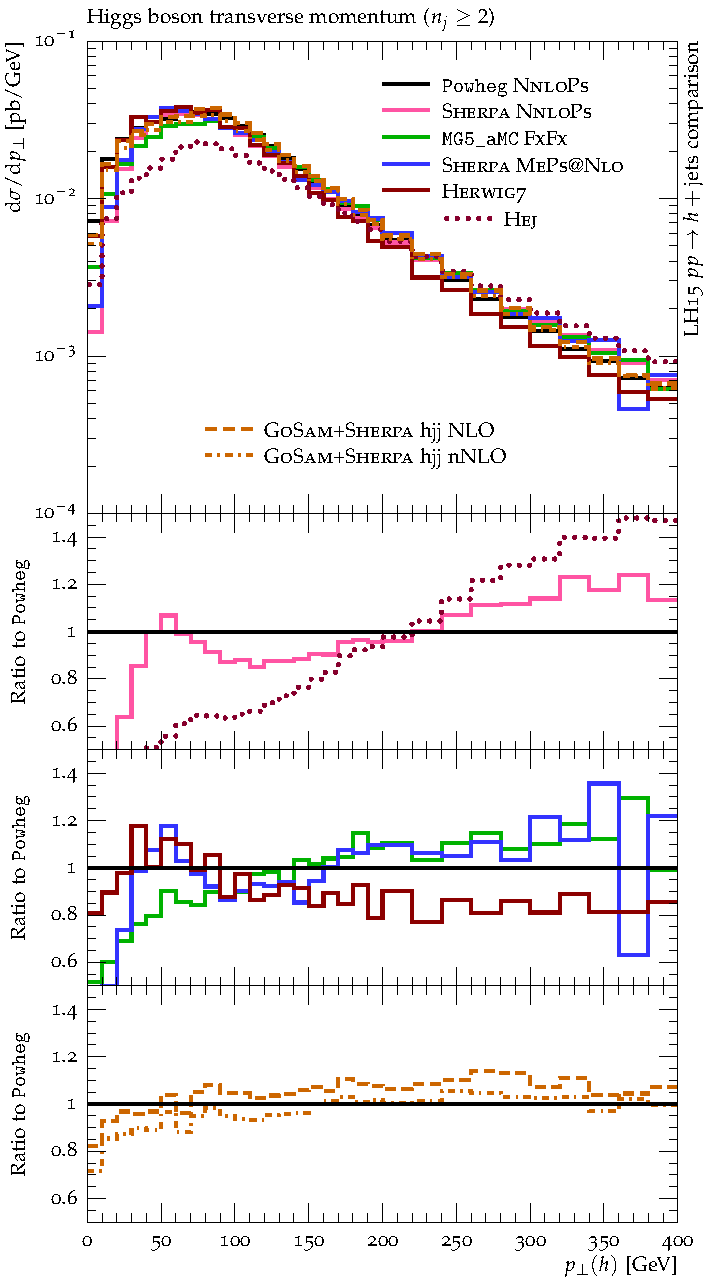
\includegraphics[width=0.47\textwidth]{figures/hjetscomp_u_H_jj_pT_incl.pdf}
  \hfill
  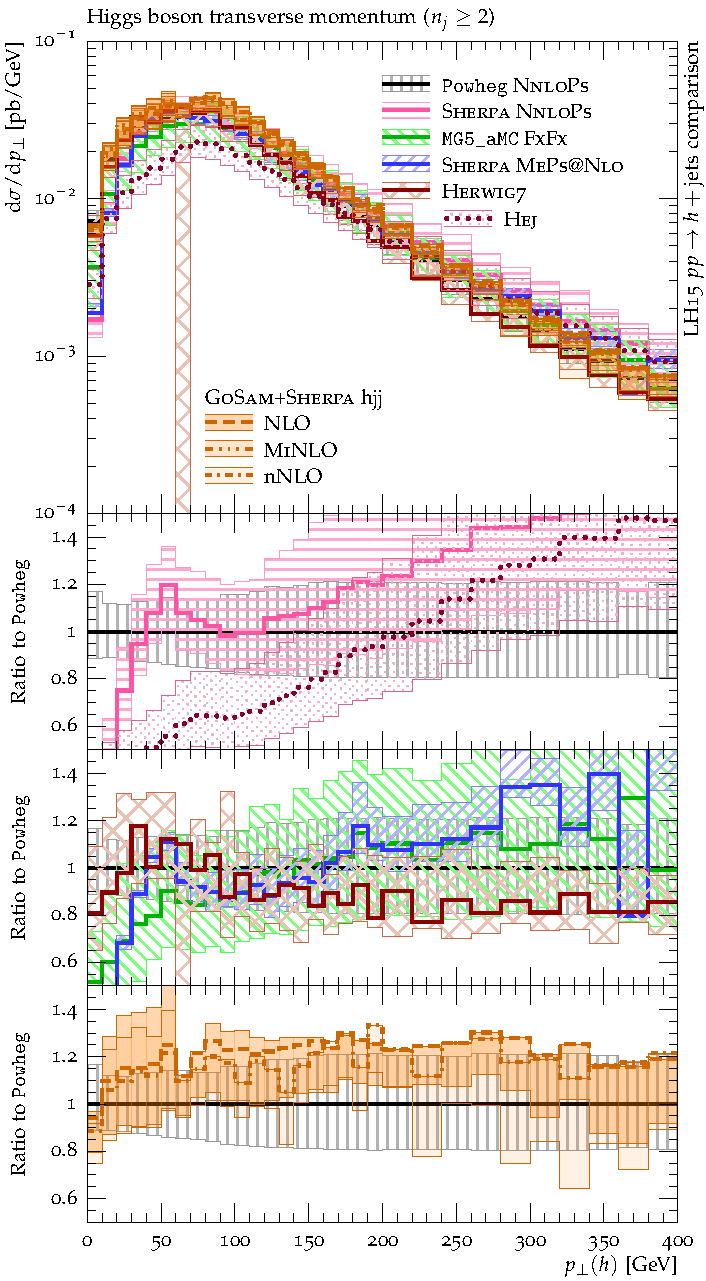
\includegraphics[width=0.47\textwidth]{figures/hjetscomp_H_jj_pT_incl.pdf}
  \caption{\label{fig:hjetscomp:results:2obs:hpt_j2pt}%
    The transverse momentum of the Higgs boson in the presence of at
    least two jets without (left) and with (right) uncertainties,
    supplemented by three ratio plots using the reference result as
    obtained from \Powheg's \NNLOPS calculation for $h$ production.
    The predictions are grouped -- from top to bottom -- according to
    the categories \NNLOPS $h$ production, ME+PS merging at NLO (at
    least up to two jets) and NLO fixed-order $hjj$ production. \Hej's
    prediction is added to the first, the \NNLOPS, subpanel.}
\end{figure}

The Higgs boson $p_\perp$ spectrum, in the presence of at least two
jets, is shown in Figure~\ref{fig:hjetscomp:results:2obs:hpt_j2pt}.
Here, varying behaviour is observed, with \MGaMC, \Sherpa and \Hej
being substantially lower than \Powheg at low $p_\perp(h)$. \Hej
clearly produces the hardest spectrum of all overshooting \Powheg by
more than 40\% at $p_\perp(h)\sim400\gev$. Harder tails are also
generated by \Sherpa \NNLOPS ($\sim30\%$), \Sherpa \MEPSatNLO and
\MGaMC ($\sim20\%$), where those two obtained from merging ME+PS at
NLO are consistent with the results emerging from the different
\GoSam+\Sherpa calculations (which basically do not differ from one
another) at high $p_\perp$. \Herwig (giving the softest spectrum)
however does not agree with the other NLO central predictions although
it remains by and large within their uncertainty envelopes. Apart from
the very first bin, the \GoSam based calculations show a rather
constant rate increase of about 20\% wrt.~\Powheg pointing to a
$K$-factor size one more or less expects for $h\pl2$-jet production.

\begin{figure}[t!]
  \centering
  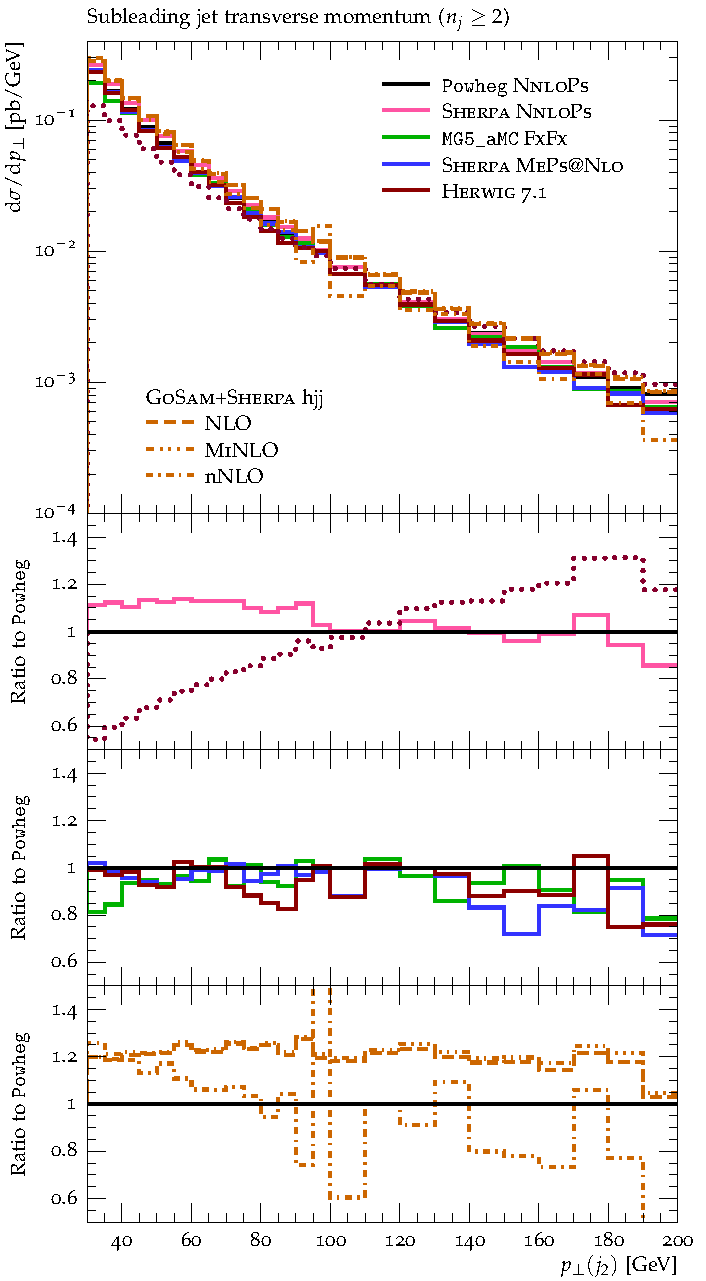
\includegraphics[width=0.47\textwidth]{figures/hjetscomp_u_jet2_pT_incl.pdf}
  \hfill
  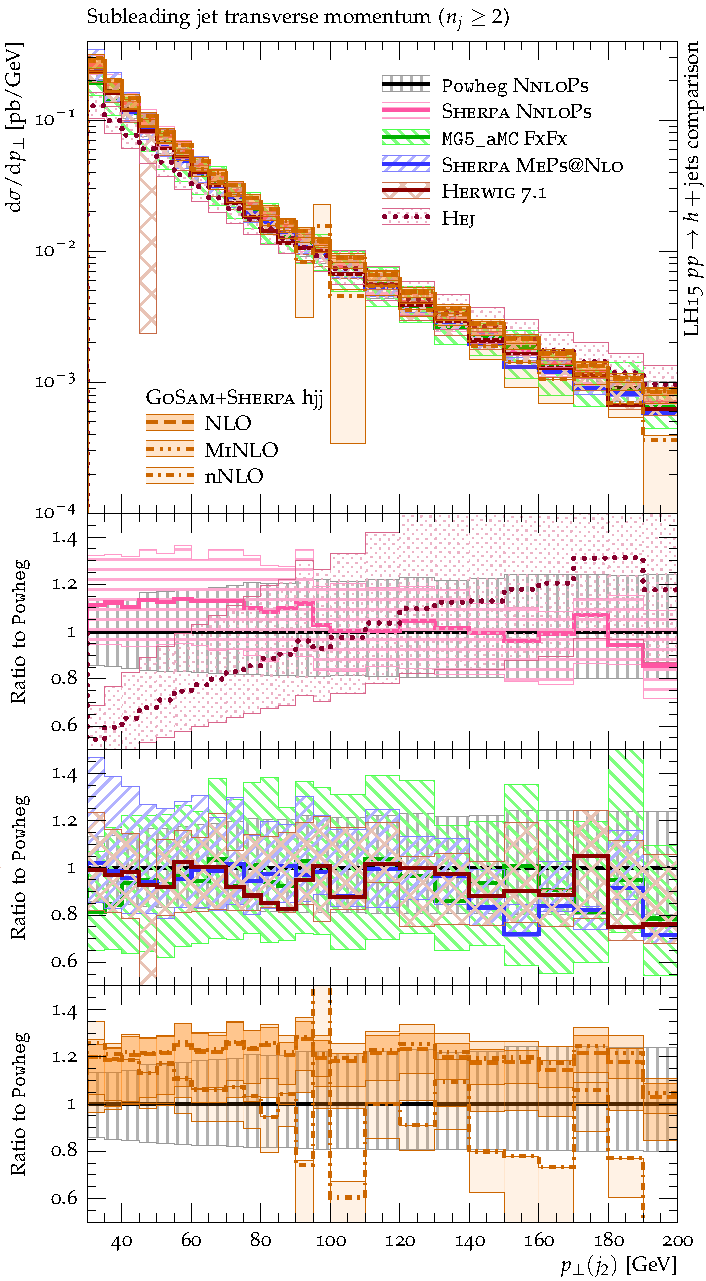
\includegraphics[width=0.47\textwidth]{figures/hjetscomp_jet2_pT_incl.pdf}
  \caption{\label{fig:hjetscomp:results:2obs:jet2_pt}%
    The subleading jet $p_\perp$ for $h\pl\ge2$-jets production shown
    without (left) and with (right) theoretical uncertainties. The
    plot layout is the same as in the previous figure.
    \Todo{the Hey legend fell off the plot.}}
\end{figure}

\begin{figure}[t!]
  \centering
  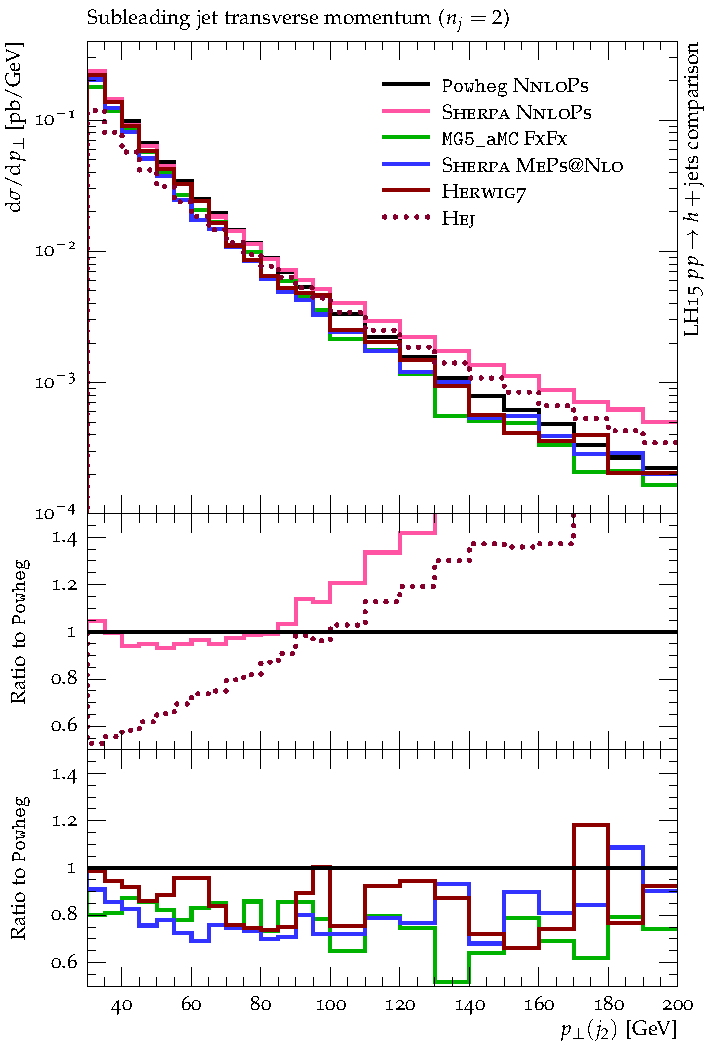
\includegraphics[width=0.47\textwidth]{figures/hjetscomp_u_jet2_pT_excl.pdf}
  \hfill
  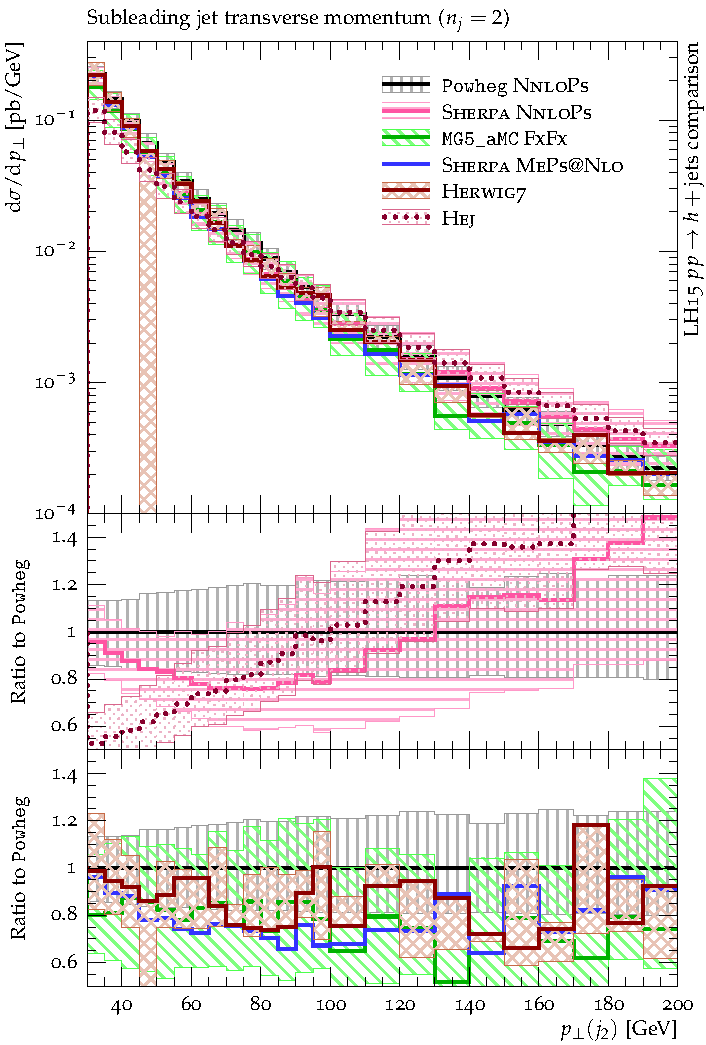
\includegraphics[width=0.47\textwidth]{figures/hjetscomp_jet2_pT_excl.pdf}
  \caption{\label{fig:hjetscomp:results:2obs:jet2_pt}%
    The subleading jet $p_\perp$ for exclusive $h\pl2$-jets production
    shown without (left) and with (right) theoretical uncertainties.
    Again, the layout is similar to that of
    Figure~\ref{fig:hjetscomp:results:2obs:hpt_j2pt} except for
    dropping the results of the NLO fixed-order $hjj$ production and
    the associated ratio subpanel.}
\end{figure}

The sub-leading jet $p_T$ for $H+\ge2$ jets is shown in the upper row
of Figure~\ref{fig:hjetscomp:results:2obs:jet2_pt}.  The agreement
among the ME+PS predictions and between the ME+PS and fixed order
predictions of gosam is better than in the case of the leading
jets. With two or more jets in the final state, meaningful predictions
to HEJ can be made for the first time.

The sub-leading jet $p_T$ for $H$ + exactly 2 jets is shown in the
lower panel of Figure~\ref{fig:hjetscomp:results:2obs:jet2_pt}.
Here, MG5, Sherpa and Herwig7 lie in reasonable agreement with each
other, but systematically lower than Powheg.

\Todo{physics?}

\begin{figure}[t!]
  \centering
  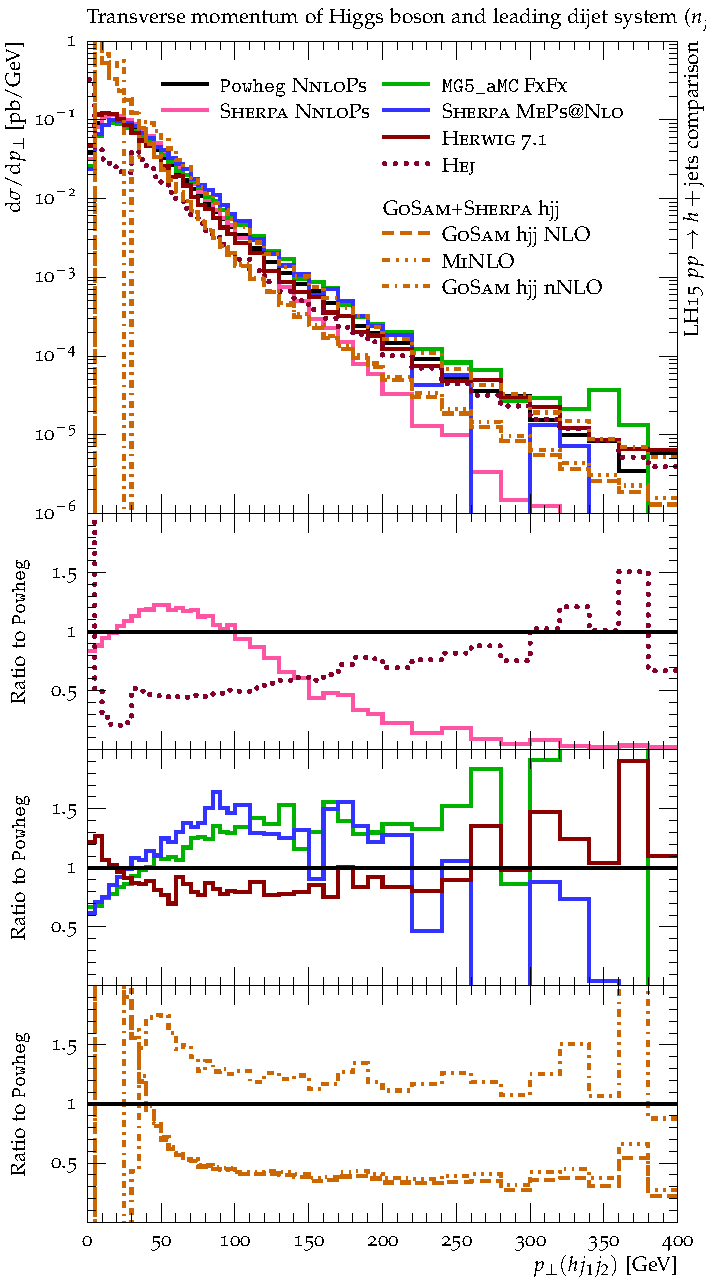
\includegraphics[width=0.47\textwidth]{figures/hjetscomp_u_Hjj_pT_incl.pdf}
  \hfill
  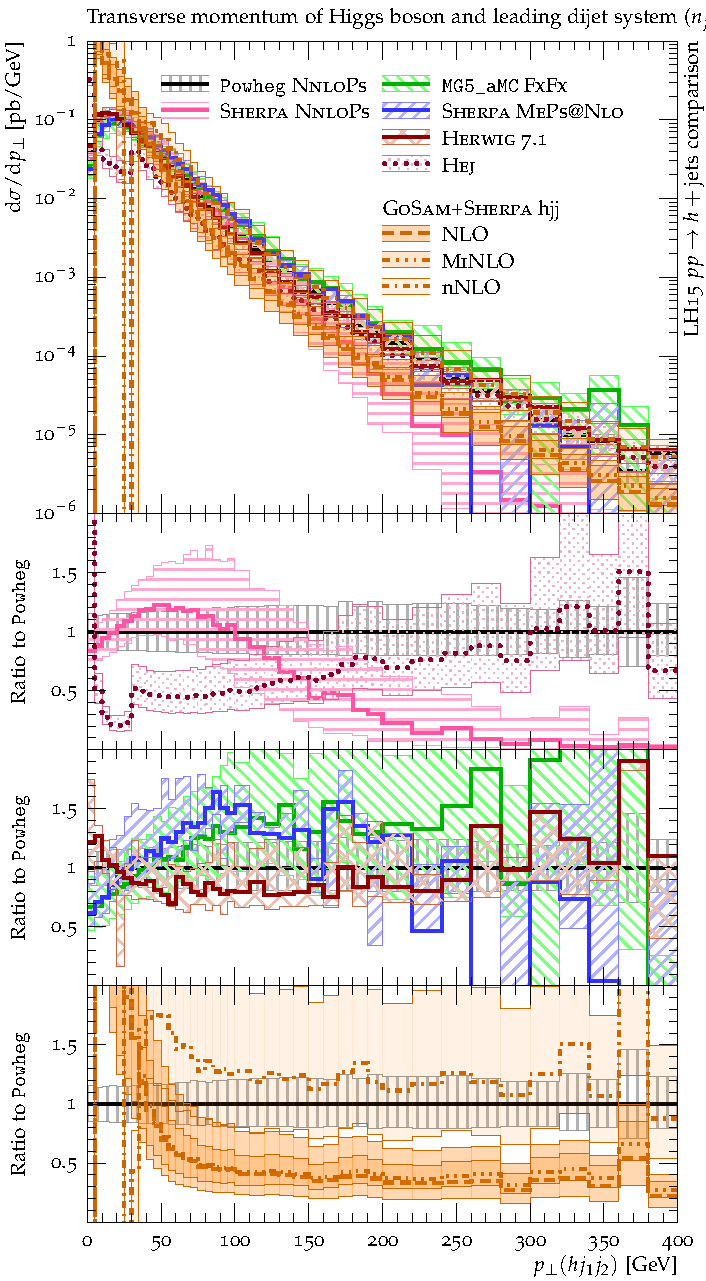
\includegraphics[width=0.47\textwidth]{figures/hjetscomp_Hjj_pT_incl.pdf}
  \caption{\label{fig:hjetscomp:results:2obs:hjj_pt}%
    The transverse momentum distribution of the Higgs boson plus two
    leading jet system, shown without (left) and with (right)
    uncertainties. The plot layout is the same as in
    Figure~\ref{fig:hjetscomp:results:2obs:hpt_j2pt}.}
\end{figure}

The transverse momentum of the Higgs boson plus two leading jet system
is shown in Figure~\ref{fig:hjetscomp:results:2obs:hjj_pt}. Varying
behavior is also observed here, with MG5 and Sherpa being having a
slope with respect to Powheg at low $p_T$ and being somewhat higher at
high $p_T$, while Herwig7 is again somewhat lower than Powheg at high
$p_T$. The gosam $H+\ge2$ jet prediction is much higher than Powheg at
low $p_T$, and significantly lower at high $p_T$.

\Todo{physics!; why does gosam have the behavior it does?}

\begin{figure}[t!]
  \centering
  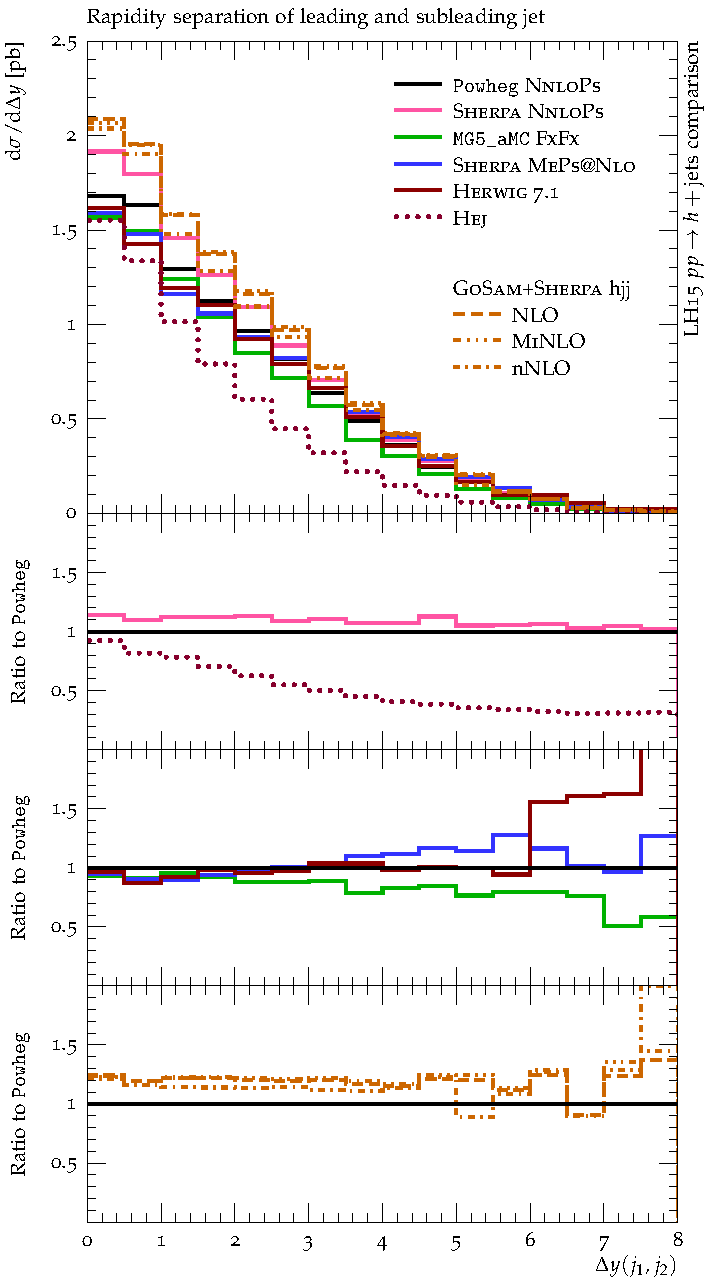
\includegraphics[width=0.47\textwidth]{figures/hjetscomp_u_deltay_jj.pdf}
  \hfill
  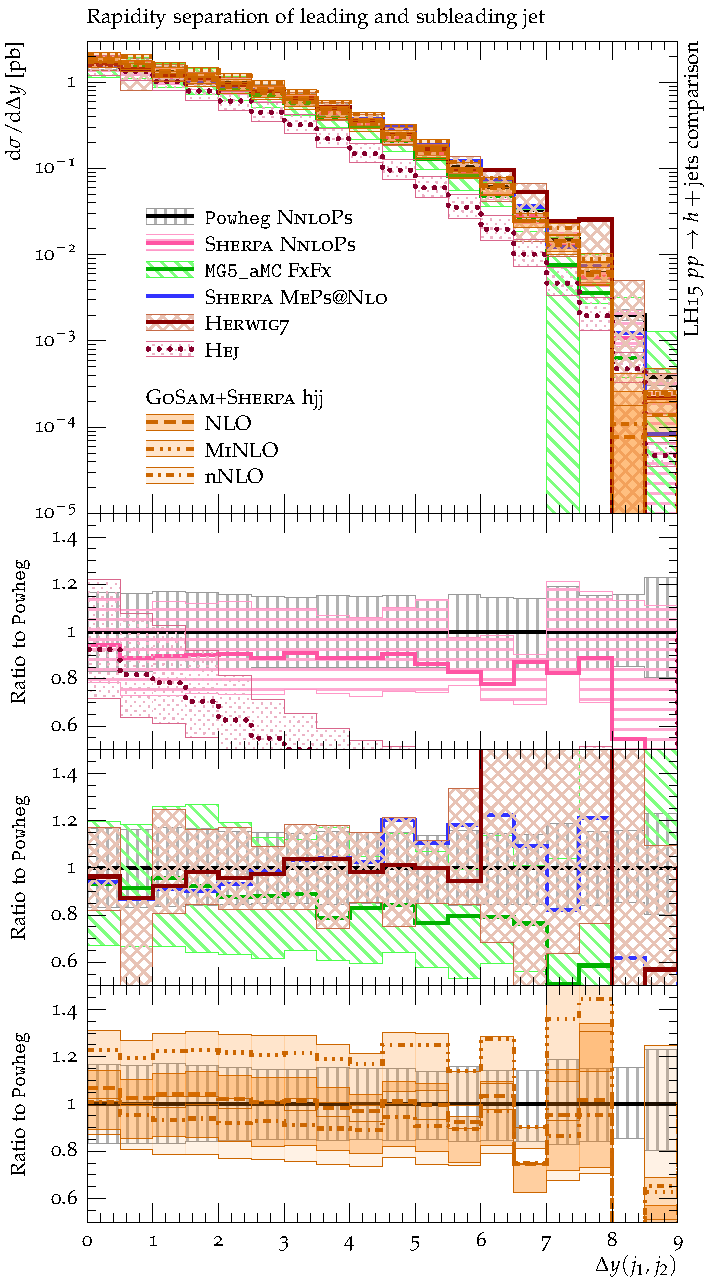
\includegraphics[width=0.47\textwidth]{figures/hjetscomp_deltay_jj.pdf}
  \caption{\label{fig:hjetscomp:results:2obs:dyjj}%
    The rapidity separation between the leading and subleading jets
    for $h\pl\ge2$-jets production, shown without (left) and with
    (right) theoretical uncertainties. The plot layout is the same as
    the one used in Figure~\ref{fig:hjetscomp:results:2obs:hpt_j2pt}.}
\end{figure}

\begin{figure}[t!]
  \centering
  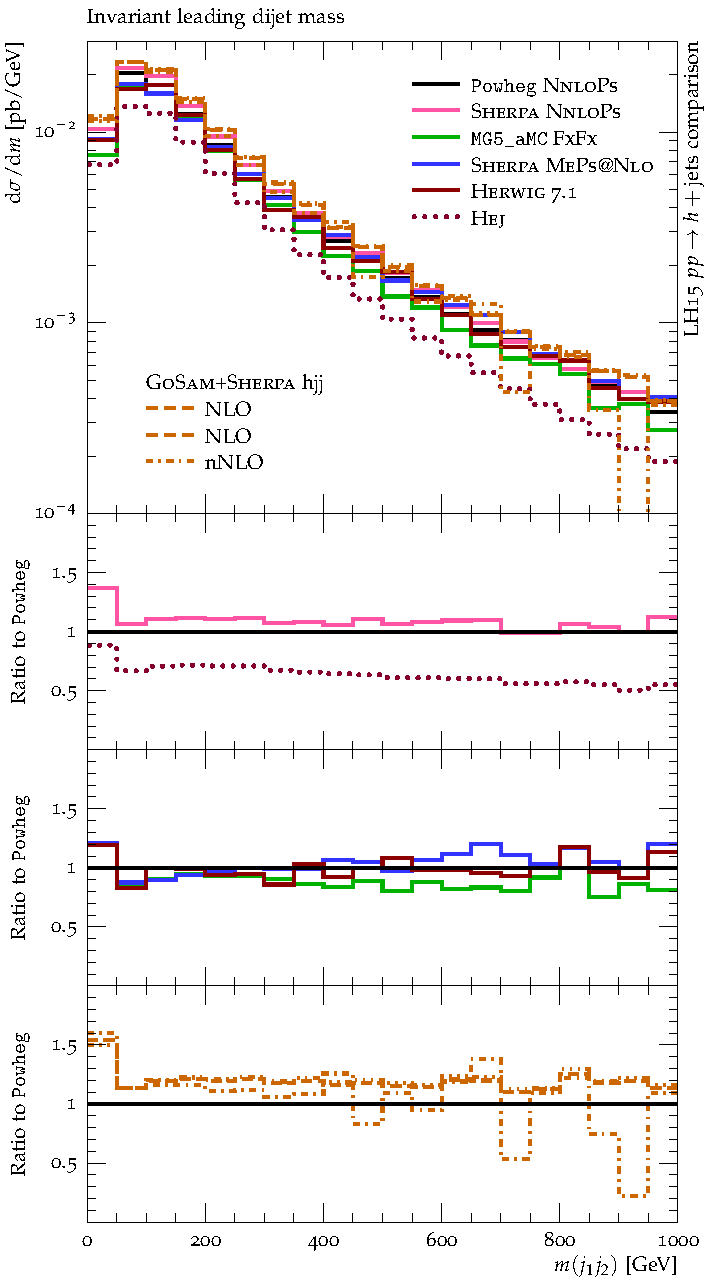
\includegraphics[width=0.47\textwidth]{figures/hjetscomp_u_dijet_mass.pdf}
  \hfill
  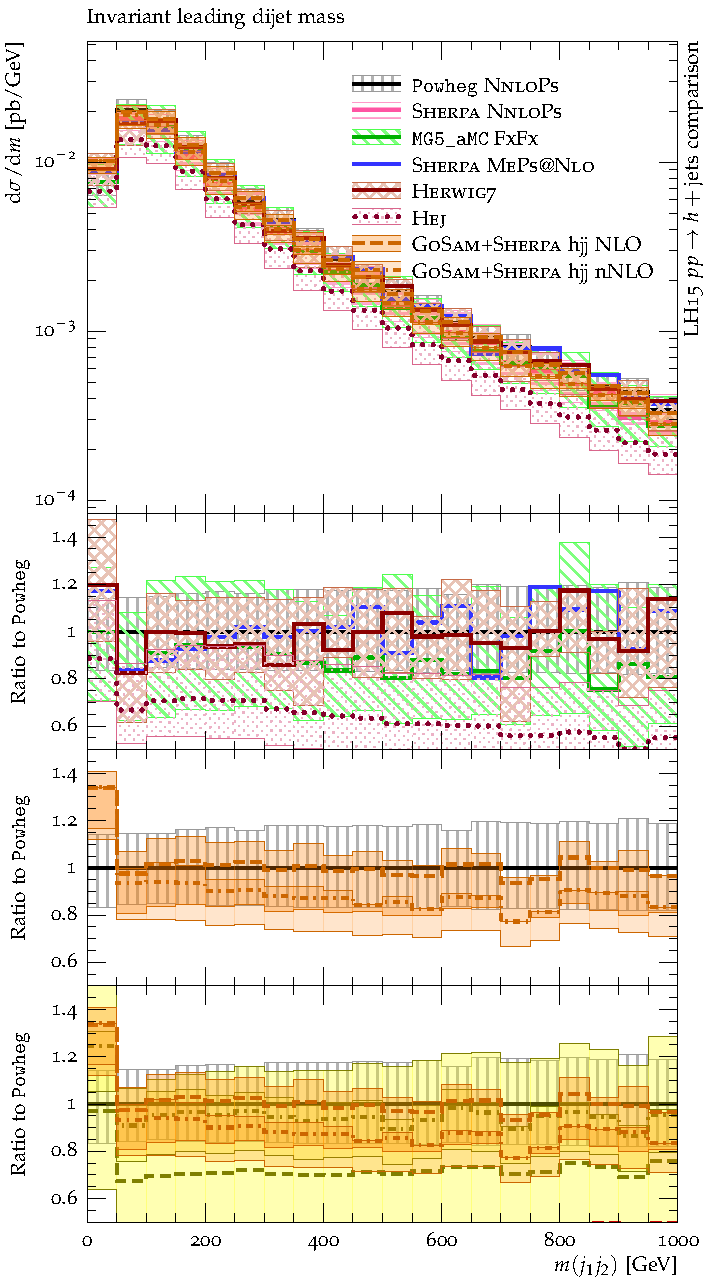
\includegraphics[width=0.47\textwidth]{figures/hjetscomp_dijet_mass.pdf}
  \caption{\label{fig:hjetscomp:results:2obs:mjj}%
    The invariant mass distribution of the leading dijet system in
    $h\pl\ge2$-jets production, shown without (left) and with (right)
    theoretical uncertainties. The plot layout is the same as the one
    used in Figure~\ref{fig:hjetscomp:results:2obs:hpt_j2pt}.}
\end{figure}

The rapidity separation between the leading and sub-leading jets is
shown in Figure~\ref{fig:hjetscomp:results:2obs:dyjj}, for $H+\ge2$
jets. MG5 is lower than Powheg at high $\Delta y$ (while Sherpa is
slightly higher).  Powheg is in good agreement with the fixed order
gosam results for $H+\ge2$ jets. Similar conclusions hold for for the
dijet mass distribution, as shown in
Figure~\ref{fig:hjetscomp:results:2obs:mjj}, although the differences
among predictions are smaller.

\begin{figure}[t!]
  \centering
  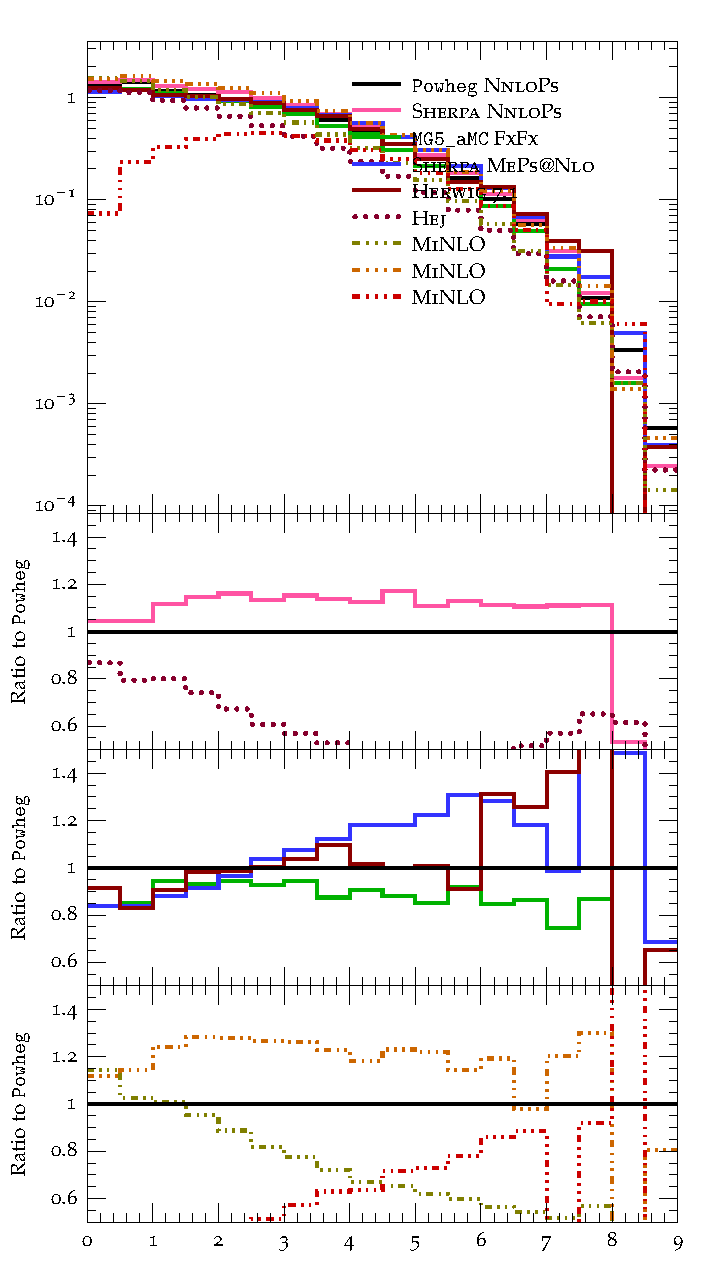
\includegraphics[width=0.47\textwidth]{figures/hjetscomp_u_jjfb_dy.pdf}
  \hfill
  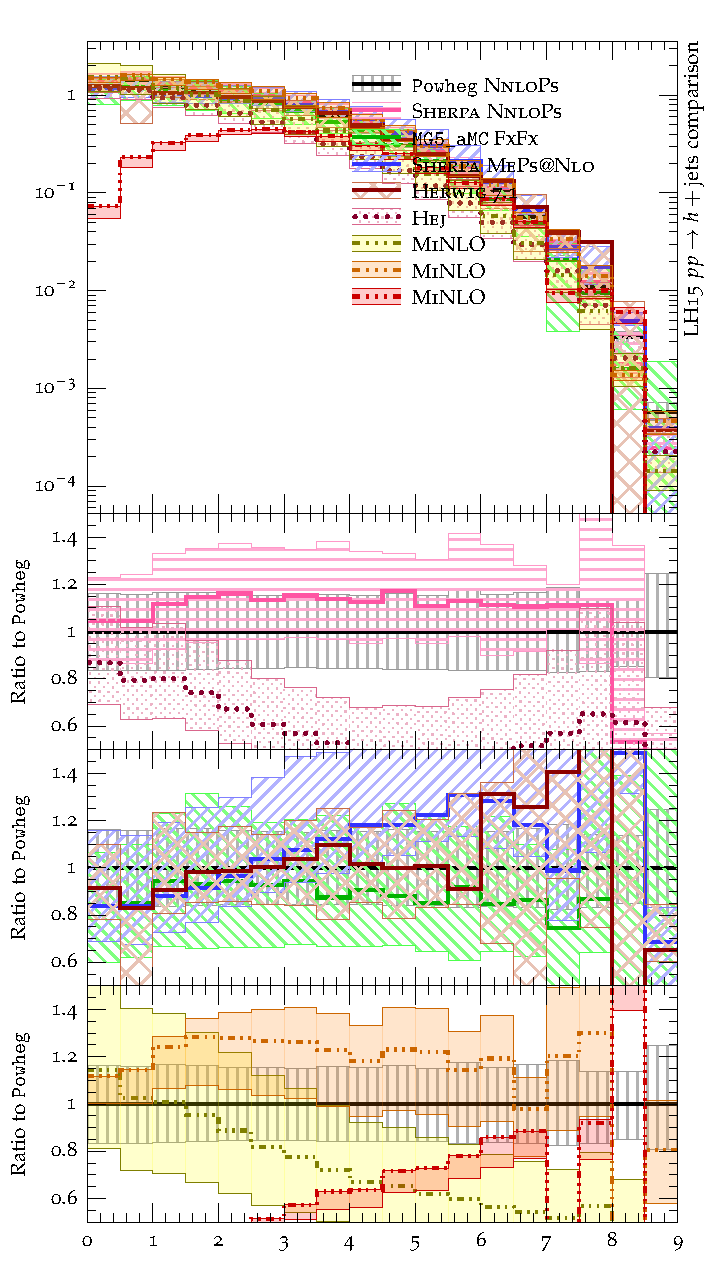
\includegraphics[width=0.47\textwidth]{figures/hjetscomp_jjfb_dy.pdf}
  \caption{\label{fig:hjetscomp:results:2obs:dyjj_fb}%
    The rapidity separation between the two most forward-backward jets
    for $H+\ge2$ jets, without (left) and with (right) uncertainties.
    \Todo{this plot doesn't seem to be up-to-date -- do we want it?}}
\end{figure}

\Todo{Do we want to show and discuss this plot? Seems outdated
  compared to all other ones:\\
  The rapidity separation between the two most forward-backward jets is
  shown in Figure~\ref{fig:hjetscomp:results:2obs:dyjj_fb}. As for the
  $p_T$-ordered distribution, MG5 is lower than Powheg at high $\Delta
  y$ while Sherpa is higher. Powheg now has a slope compared to the
  Gosam NLO results, but, interestingly, not compared to the nNLO
  results.
}

\begin{figure}[t!]
  \centering
  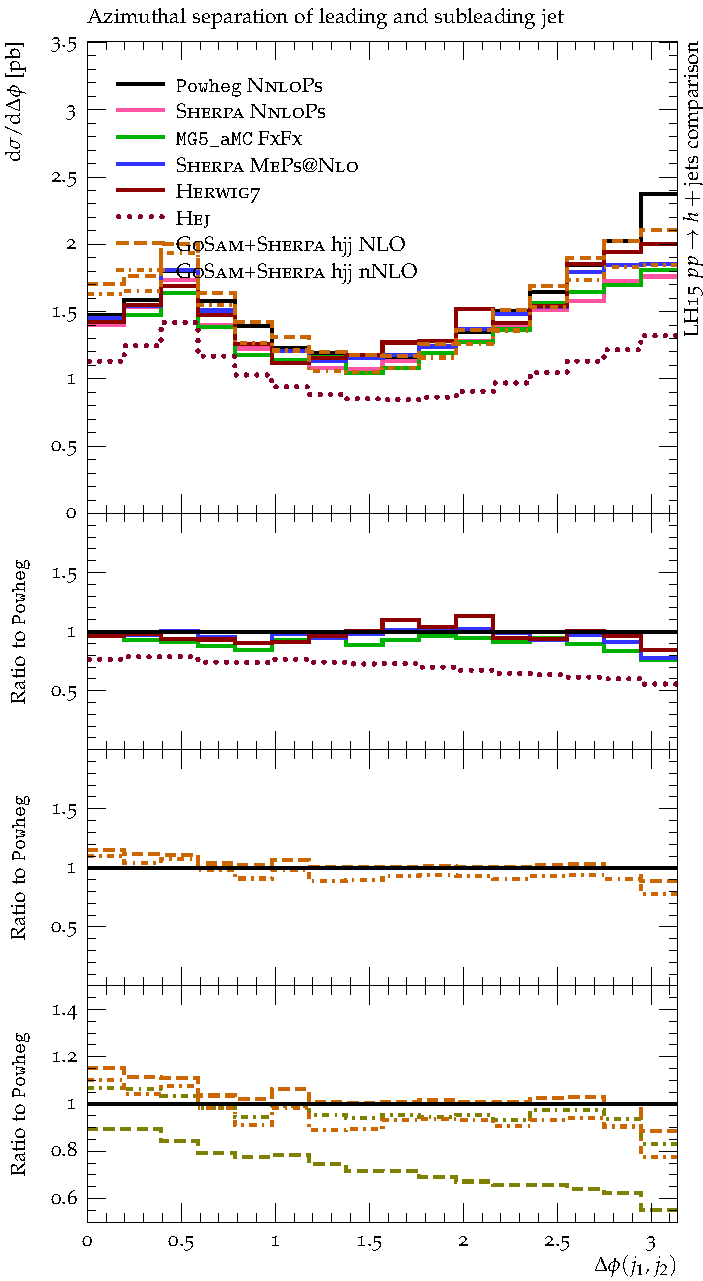
\includegraphics[width=0.47\textwidth]{figures/hjetscomp_u_deltaphi_jj_incl.pdf}
  \hfill
  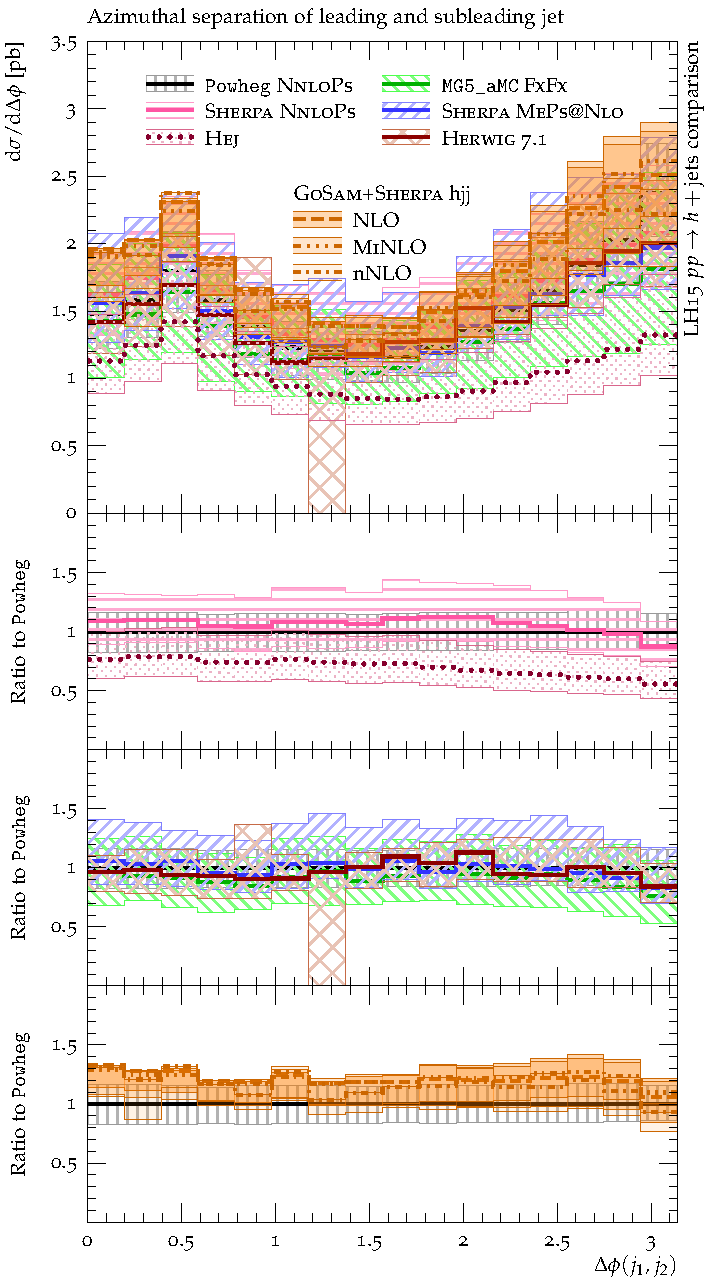
\includegraphics[width=0.47\textwidth]{figures/hjetscomp_deltaphi_jj_incl.pdf}
  \caption{\label{fig:hjetscomp:results:2obs:dphi_jj}%
    The $\Delta\phi$ separation between the two leading jets for
    $h\pl\ge2$-jets production, presented without (left) and with
    (right) the associated theoretical uncertainties. Again, the
    plot layout is the same as the one used in
    Figure~\ref{fig:hjetscomp:results:2obs:hpt_j2pt}.}
\end{figure}

The $\Delta\phi$ separation between the two leading jets is shown in
Figure~\ref{fig:hjetscomp:results:2obs:dphi_jj}. All predictions are
in good agreement with each other, except for HEJ, which has a leading
order normalization. Similar distributions (and agreement) are
observed if the two most forward-backward jets are chosen instead.



\clearpage
\subsection{VBF observables}
\label{sec:hjetscomp:results:VBFobs}

A situation where Higgs boson production in gluon fusion primarily
serves as background is found in analyses intended to measure its
couplings to weak vector bosons. To enhance the relative contribution
of processes where the Higgs boson production proceeds through weak
vector boson fusion (VBF), additional cuts are placed on the so-called
tagging jets. The tagging jets themselves can now be defined in
multiple ways. In the study performed during the Les Houches 2013
workshop \cite{AlcarazMaestre:2012vp}, the standard leading
($p_\perp$-ordered) jet selection was supplemented with the
forward-backward selection defining the pair of jets with the largest
rapidity separation as tagging jets. Another strategy using the
highest invariant mass jet pair was also studied more recently
\cite{Greiner:2015jha}.

%In the present study, we generalised these 
%definitions, defining the tagging jets as the leading pair of 
%$p_\perp$-ordered jets which fulfils the thereupon applied cuts. 
%Of course, differences between the schemes only manifest themselves in 
%the presence of at least three jets and are, thus, formally of higher 
%order. Numerically, however, they can have a major impact and their 
%choice depends on the physics aims of the analysis to be performed. 

In this analysis, the leading and subleading jets are required to have
a mass greater than $400\gev$ and a rapidity separation greater than
$2.8$. This set of cuts is referred to as VBF cuts. An alternative set
of cuts (VBF2) requires that any two jets satisfy the above
requirements. For many observables, the distributions are similar for
the two cases, and only the VBF cut scenario will be presented.
%In our analysis, requiring the tagging jet invariant mass and rapidity 
%separation to be in excess of $400\,\gev$ and $2.8$, respectively, 
%prepares the typical VBF kinematics. Now, the contamination of these 
%observables with the irreducible background of Higgs produced in gluon 
%fusion is a key quantity in the accuracy of the extraction of the coupling 
%parameters. We thus proceed to analyse the congruence of the different 
%descriptions of a selection of key observables with the standard tagging 
%jet using the leading and sub-leading $p_\perp$-ordered jets.
Results for the alternative choice can be found at the project's
webpage \cite{webpage}.

%\begin{figure}[t!]
%  \centering
%  \begin{minipage}{0.47\textwidth}
%    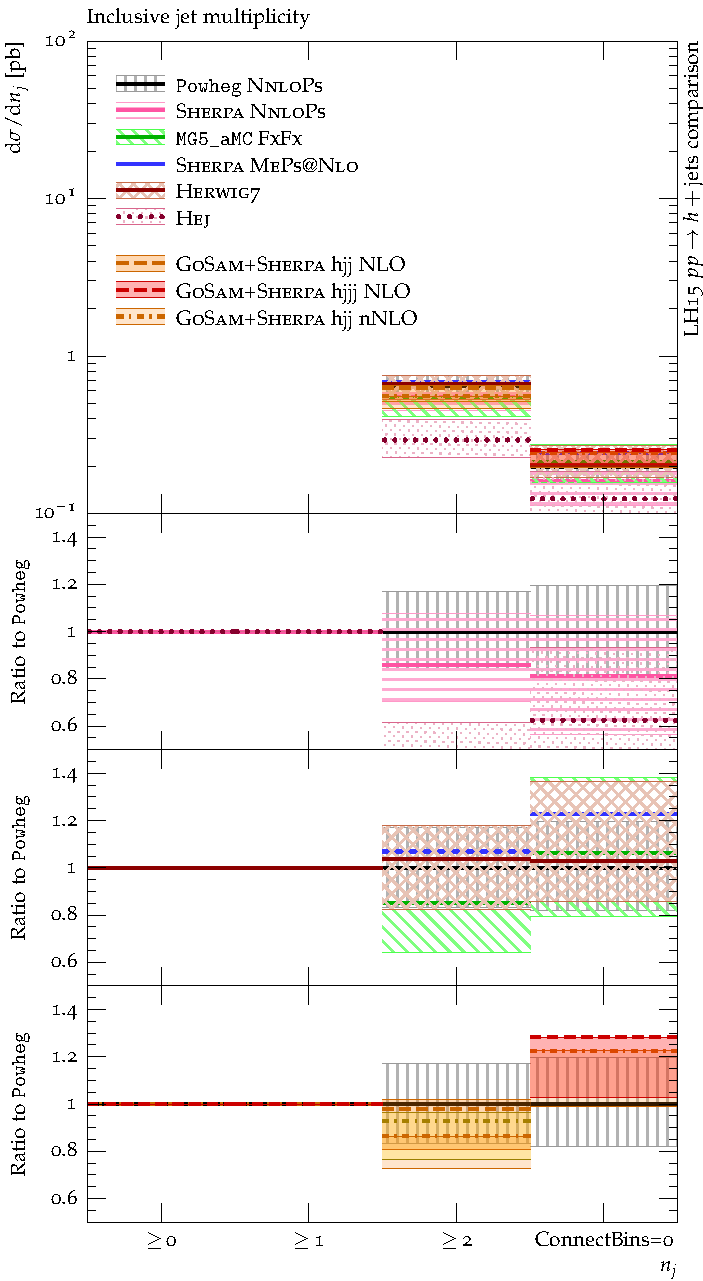
\includegraphics[width=\textwidth]{figures/hjetscomp_NJet_incl_30_VBF.pdf}
%  \end{minipage}
%  \hfill
%  \begin{minipage}{0.47\textwidth}
%    \lineskip-1.35pt
%    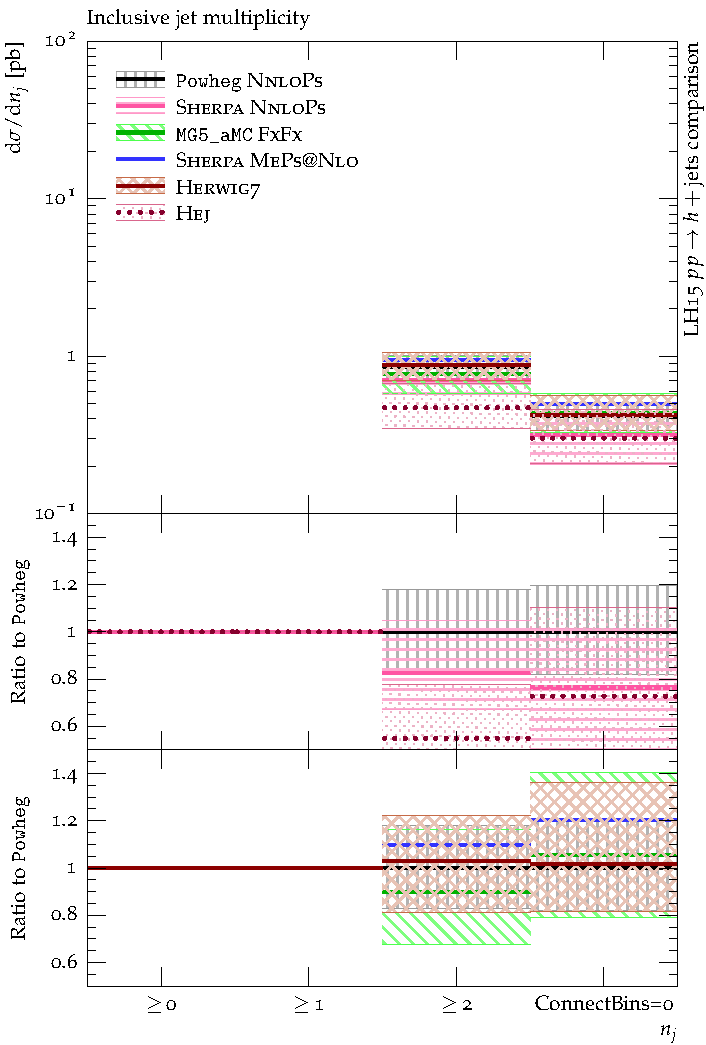
\includegraphics[width=\textwidth]{figures/hjetscomp_NJet_incl_30_VBF2.pdf}\\
%    
\includegraphics[width=\textwidth]{figures/ratiopanelplaceholder.pdf}
%  \end{minipage}
%  \caption{
%    The inclusive jet multiplicities after the application of the VBF 
%    cuts standard leading tagjet definition (VBF, left) and 
%    the generalised leading tagjet definition (VBF2, right).
%    \label{fig:hjetscomp:results:inclobs:njets_VBF}
%  }
%\end{figure}

\begin{figure}[t!]
  \centering
  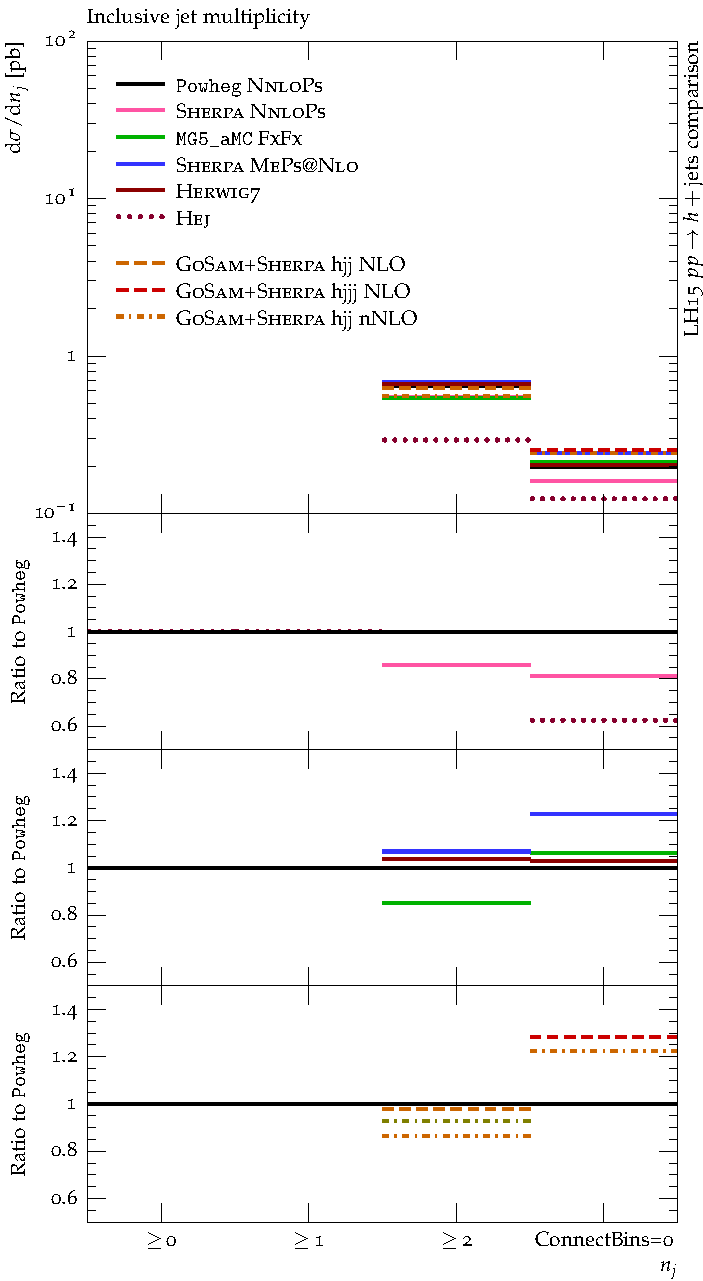
\includegraphics[width=0.47\textwidth]{figures/hjetscomp_u_NJet_incl_30_VBF.pdf}
  \hfill
  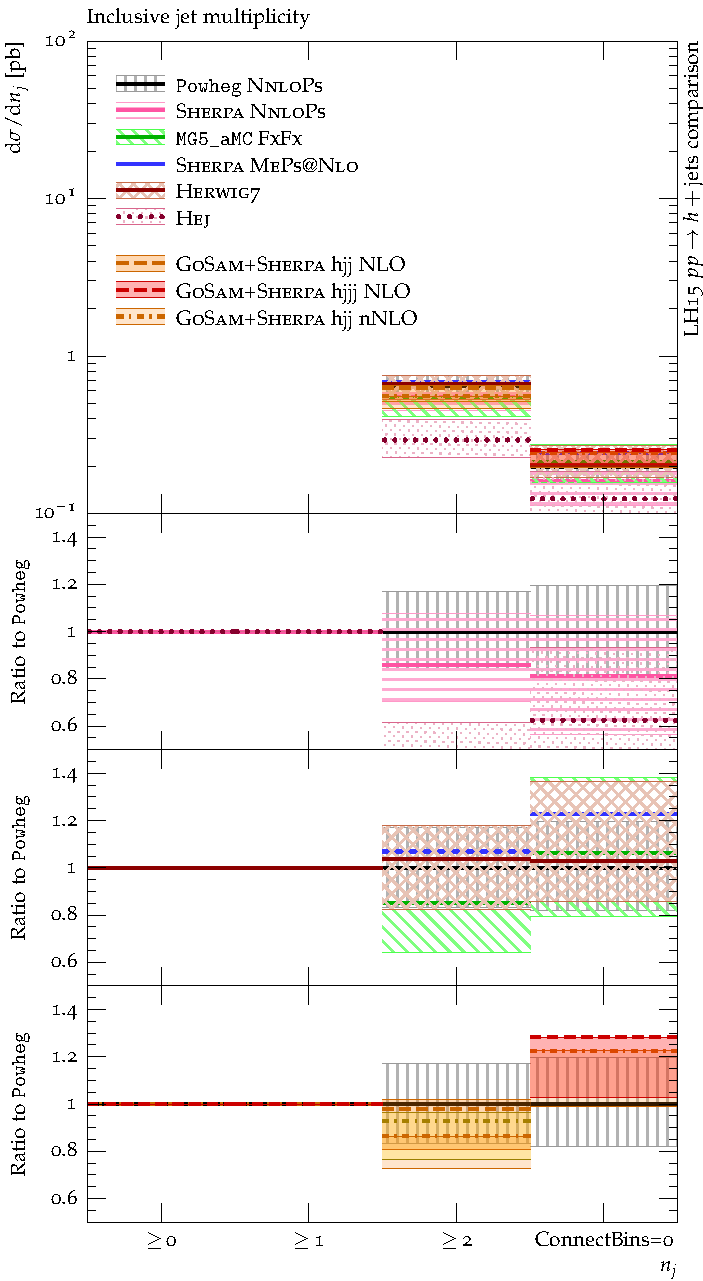
\includegraphics[width=0.47\textwidth]{figures/hjetscomp_NJet_incl_30_VBF.pdf}
  \caption{\label{fig:hjetscomp:results:inclobs:njets_VBF}%
    The inclusive jet multiplicities after imposing the leading
    tag-jets definition (see text for the details of the `VBF'
    selection), shown without (left) and with (right) uncertainties.}
\end{figure}

\begin{figure}[t!]
  \centering
  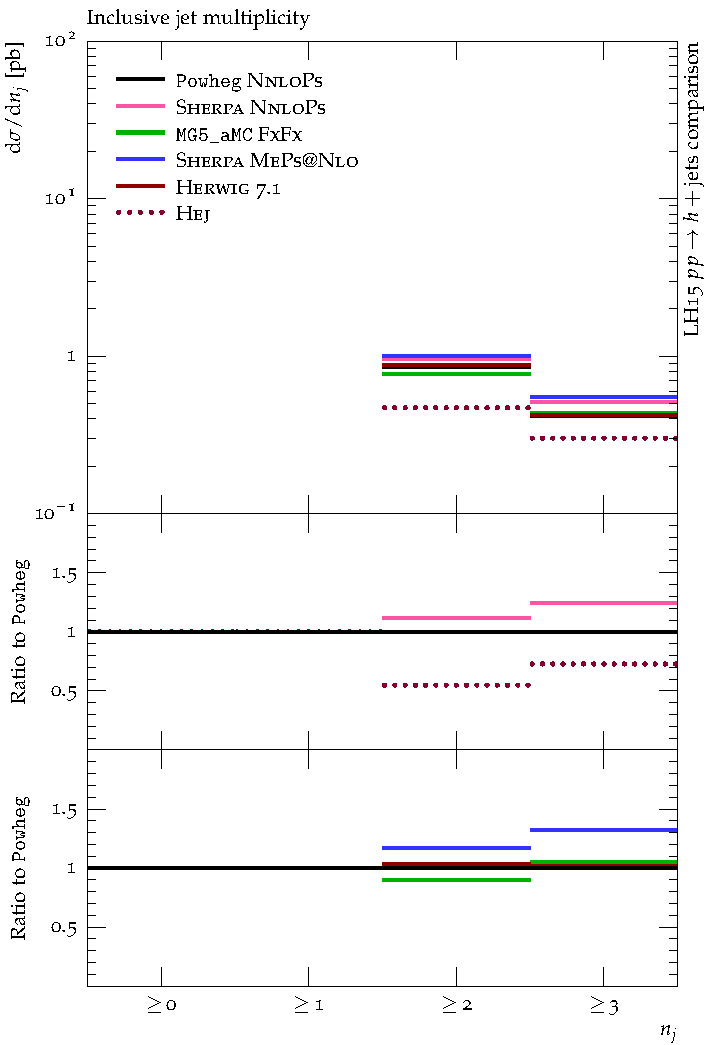
\includegraphics[width=0.47\textwidth]{figures/hjetscomp_u_NJet_incl_30_VBF2.pdf}
  \hfill
  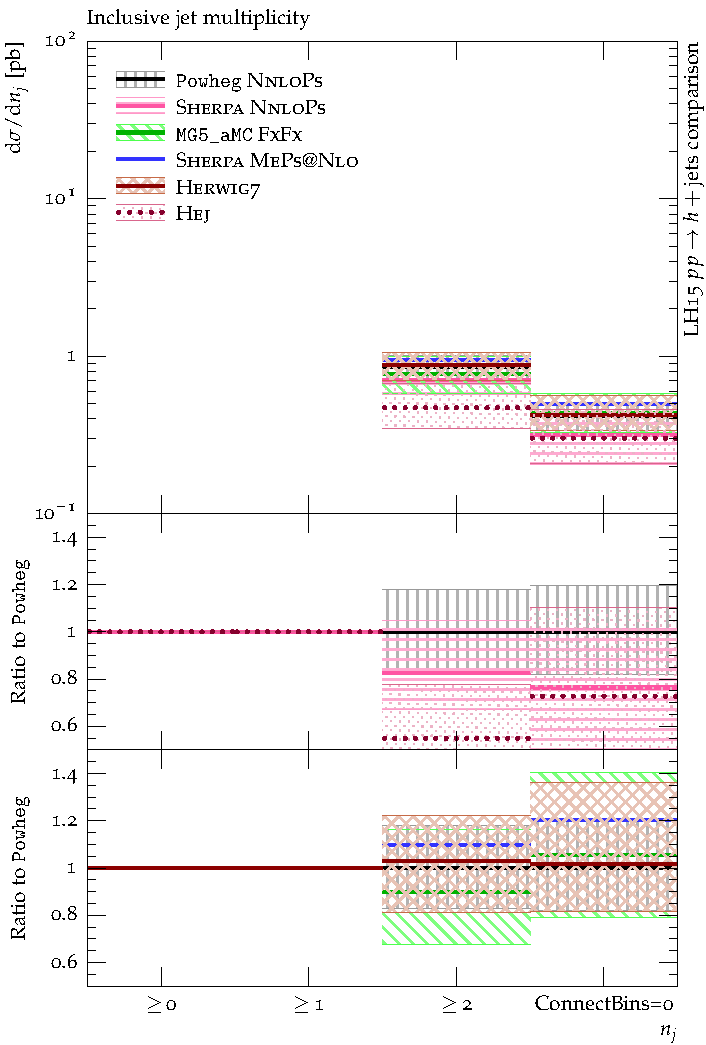
\includegraphics[width=0.47\textwidth]{figures/hjetscomp_NJet_incl_30_VBF2.pdf}
  \caption{\label{fig:hjetscomp:results:inclobs:njets_VBF2}%
    The inclusive jet multiplicities after the application of the `VBF2'
    tag-jets cuts (see text for the definition), shown without (left)
    and with (right) uncertainties.}
\end{figure}

%We start by examining the inclusive jet multiplicity distributions after
%the application of the above detailed VBF cuts in
The inclusive jet multiplicity distributions after the application of
the VBF (VBF2) cuts are shown in
Figure~\ref{fig:hjetscomp:results:inclobs:njets_VBF}
(Figure~\ref{fig:hjetscomp:results:inclobs:njets_VBF2}).  The
hierarchy observed is essentially the same as for the inclusive jet
multiplicity distribution without any cuts. The differences among the
predictions are slightly smaller with the VBF2 cuts than with the VBF
cuts.  In both cases, the \NNLOPS calculations are again in very good
agreement with \Sherpa \NNLOPS. \Todo{Correct?}
% allowing for a larger uncertainty which is driven
%by the partially evaluated resummation uncertainty not assessed in \Powheg.
\Hej predicts only about 50\% of the cross section of \NNLOPS.
%Comparing with the inclusive dijet
%cross sections of Figure \ref{fig:hjetscomp:results:inclobs:njets}
%Nonetheless, the number of gluon fusion events passing the VBF
%selection criteria it therefore predicts a significantly smaller
%VBF cut efficiency.
For the $\ge2$-jet bin, the NLO merged predictions vary from a 20\%
smaller cross section (\MGaMC) to a 20\% larger cross section (\Sherpa
\MEPSatNLO); both are at the edge of the \NNLOPS uncertainty
band. Interestingly, their uncertainty is of similar size as \NNLOPS,
$\sim$20\%, despite being of NLO accuracy for these observables (only
LO for \NNLOPS). This hints at underestimated uncertainties of the
\NNLOPS calculations for this observable. The NLO and \Minlo
\GoSam{}+\Sherpa predictions are also 20\% larger than the \NNLOPS
result in the $\ge 2$ jet bin, close to the \Sherpa \MEPSatNLO
prediction, while the \Loopsim prediction is about 5\% higher than the
\NNLOPS predictions.
%Their uncertainties are all one-sided and with about 20\%
%of the same relative size as the NLO multijet merged uncertainties.
More differences are apparent after requiring a third jet. The NLO and
\Minlo \GoSam{}+\Sherpa predictions are substantially larger than the
\NNLOPS predictions and the prediction from \MGaMC, but in better
agreement with that from \Sherpa \MEPSatNLO. This is expected given
the NLO normalization present in those calculations (NLO,\Minlo
\GoSam{}+\Sherpa, \Sherpa \NNLOPS). The third jet arises from parton
showering in the \NNLOPS calculations and from a leading order matrix
element in \MGaMC.
%The \NNLOPS calculations drop with respect to
%all other ones due to their thrid jet desription coming entirely from
%their parton showers' soft-collinear approximation. Otherwise, the
%picture remains unchanged. The fixed-order cross-section again is in
%rough agreement with the \Sherpa \MEPSatNLO one, their uncertainties,
%however, manifesting themselves differently.

\Todo{physics!; why don't Powheg, MG5 have larger uncertainties in the
  third jet bin?}

%% We start by examining the inclusive jet multiplicity distributions after 
%% the application of the above detailed VBF cuts in 
%% Figure~\ref{fig:hjetscomp:results:inclobs:njets_VBF}. The hierarchy
%% is essentially the same as for the inclusive jet multiplicity
%% distribution without any cuts. The differences among the predictions
%% are somewhat smaller with the VBF2 cuts than with the VBF cuts. 
%% In both cases, the \NNLOPS calculations are again in very good agreement 
%% with \Sherpa \NNLOPS allowing for a larger uncertainty which is driven 
%% by the partially evaluated resummation uncertainty not assessed in \Powheg. 
%% \Hej throughout predicts only about 50\% of the cross section of the the 
%% \NNLOPS predicted cross section. Comparing with the inclusive dijet 
%% cross sections of Figure \ref{fig:hjetscomp:results:inclobs:njets}
%% Nonetheless, the number of gluon fusion events passing the VBF 
%% selection criteria it therefore predicts a significantly smaller 
%% VBF cut efficiency. The NLO merged predictions vary from a 20\% 
%% smaller number of events (\MGaMC) to a 20\% larger number of events 
%% (\Sherpa \MEPSatNLO) surviving the event selection, both at the edge of 
%% the \NNLOPS uncertainty band. Interestingly, their uncertainty is of 
%% similar size as the \NNLOPS on, $\sim$20\%, despite being of NLO 
%% accuracy for these observables (only LO for \NNLOPS). This hints 
%% at the underestimated uncertainties of the \NNLOPS calculations for 
%% this observable. The NLO and \Minlo \GoSam{}+\Sherpa calculations are 
%% also 20\% larger than the \NNLOPS result, close to the \Sherpa \MEPSatNLO 
%% prediction, while the \Loopsim prediction exceeds the \NNLOPS ones only 
%% by about 5\%. Their uncertainties are all one-sided and with about 20\% 
%% of the same relative size as the NLO multijet merged uncertainties. 
%% Requiring a third jet sees the \NNLOPS calculations drop with respect to 
%% all other ones due to their thrid jet desription coming entirely from 
%% their parton showers' soft-collinear approximation. Otherwise, the 
%% picture remains unchanged. The fixed-order cross-section again is in 
%% rough agreement with the \Sherpa \MEPSatNLO one, their uncertainties,
%% however, manifesting themselves differently.

\begin{figure}[t!]
  \centering
  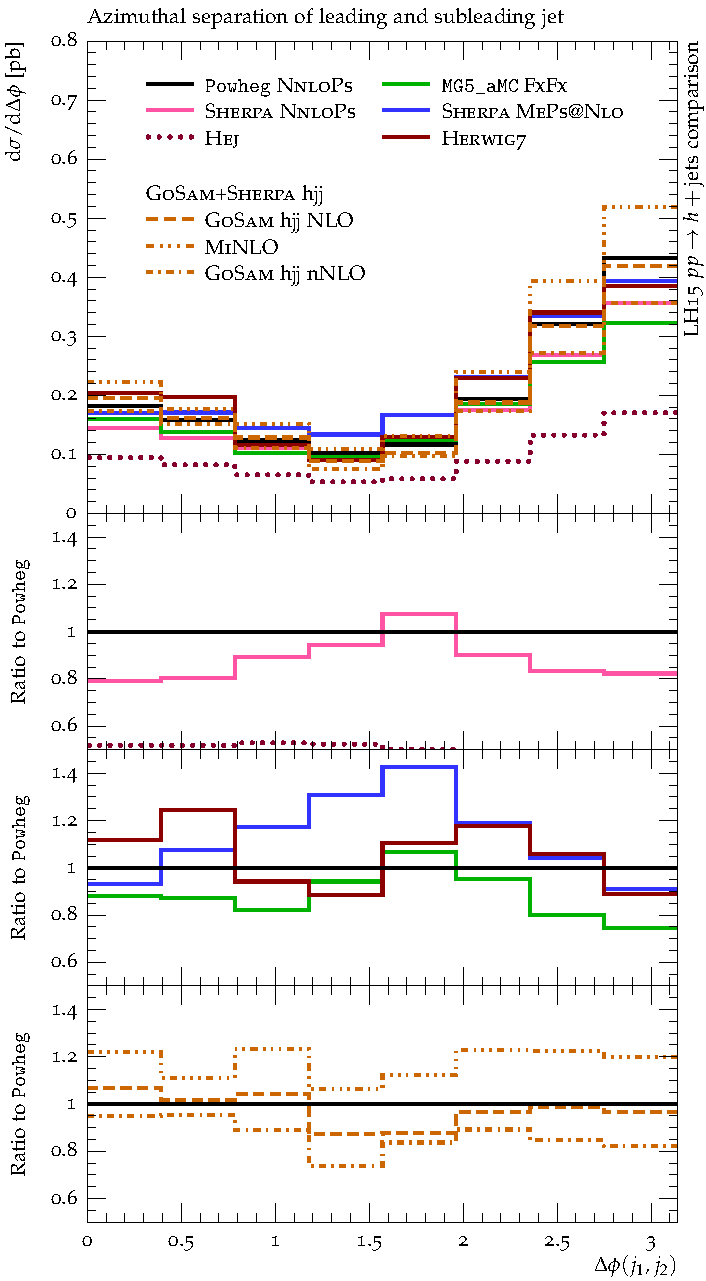
\includegraphics[width=0.47\textwidth]{figures/hjetscomp_u_deltaphi_jj_VBF.pdf}
  \hfill
  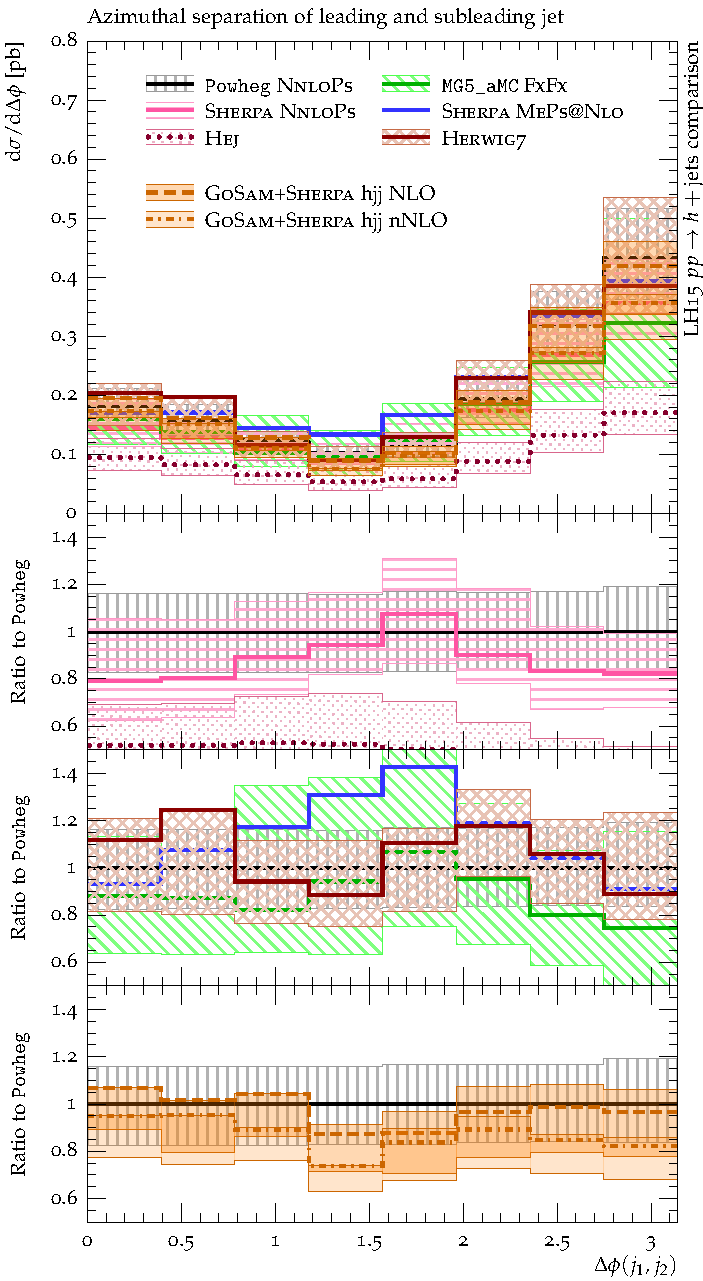
\includegraphics[width=0.47\textwidth]{figures/hjetscomp_deltaphi_jj_VBF.pdf}
  \caption{\label{fig:hjetscomp:results:VBFobs:dphijj}%
    The azimuthal separation of the leading jet pair (VBF cuts) shown
    without (left) and with (right) uncertainities in $h\pl\ge2$-jet
    production.}
\end{figure}

The $\Delta\phi$ separation between the two tagging jets is a crucial
observable in VBF measurements.
%Its gluon fusion contribution is
%similarly described by all calculations with the uncertainties being
In general, there is good agreement among the various predictions for
this observable, with the caveat
%$\sim$20\% throughout.
that \Sherpa, in both its \NNLOPS and its \MEPSatNLO forms, predict a
shallower dip at $\Delta\phi(j_1,j_2)\approx\tfrac{\pi}{2}$, something
that can be traced to its parton shower. Similar distributions (and
agreement) are observed if the generalised tagging jet definition
(VBF2) is used.

\Todo{physics!; I took the phi2 predictions out; do we want to do that?}

%% The $\Delta\phi$ separation between the two leading jets is a crucial 
%% observable in the VBF measurements. Its gluon fusion contribution is 
%% similarly described by all calculations with the uncertainties being 
%% $\sim$20\% throughout. Noteworthy is only the fact that \Sherpa, both 
%% its \NNLOPS and its \MEPSatNLO calculations, predict a shallower dip 
%% at $\Delta\phi(j_1,j_2)\approx\tfrac{\pi}{2}$, a fact that can be 
%% traced to its parton shower. Similar distributions (and agreement) 
%% are observed if the generalised tagging jet definition is used.

%% \begin{figure}[t!]
%%   \centering
%%   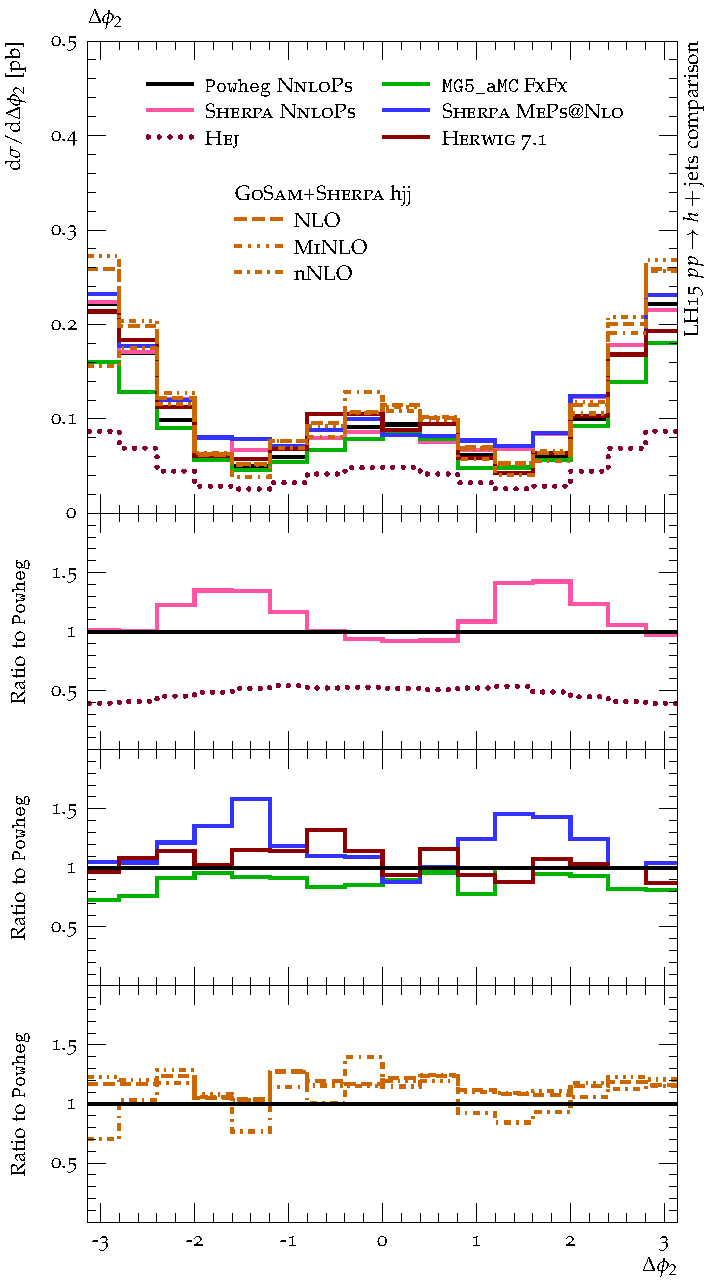
\includegraphics[width=0.47\textwidth]{figures/hjetscomp_u_deltaphi2_VBF.pdf}
%%   \hfill
%%   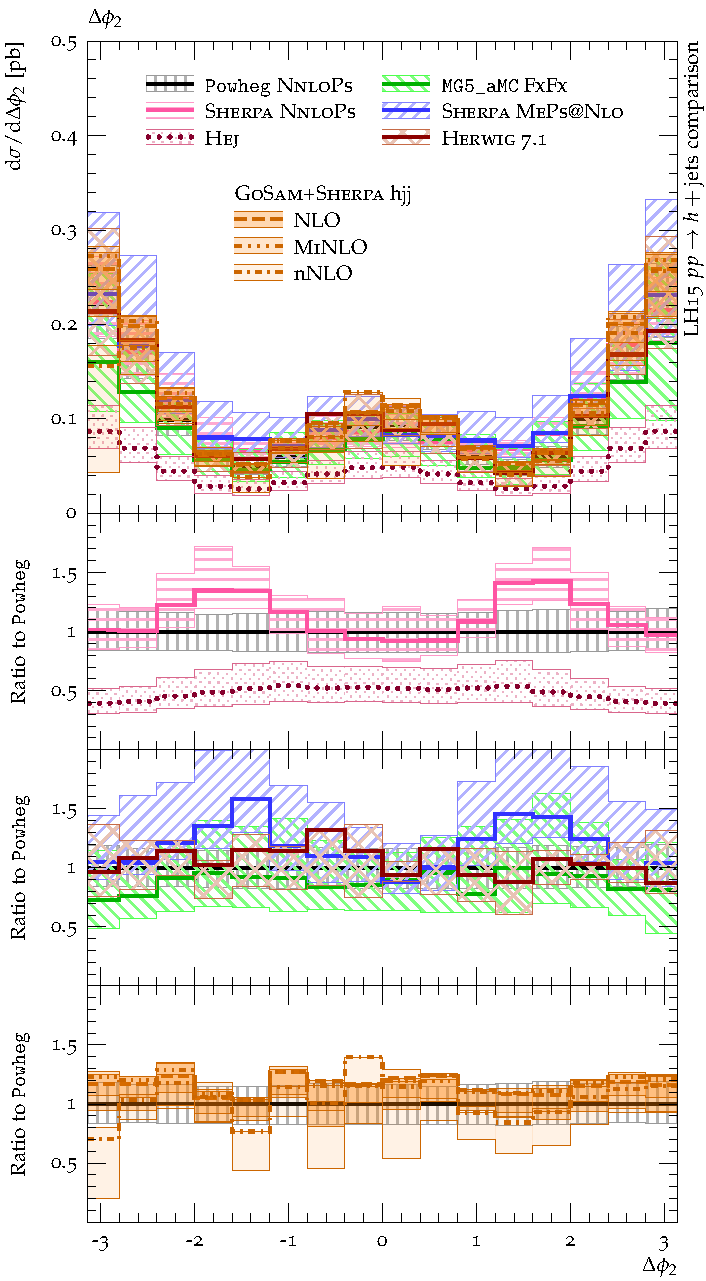
\includegraphics[width=0.47\textwidth]{figures/hjetscomp_deltaphi2_VBF.pdf}
%%   \caption{
%%     Azimuthal separation of the leading jet pair (left) and 
%%     $\Delta\phi_2$ (right) after applying VBF cuts in $H+\ge2$ jet
%%     production.
%%     \label{fig:hjetscomp:results:VBFobs:phi2}
%%   }
%% \end{figure}

%% $\Delta\phi_2$



\clearpage
\subsection{Multijet observables}
\label{sec:hjetscomp:results:mjobs}

\begin{figure}[t!]
  \centering
  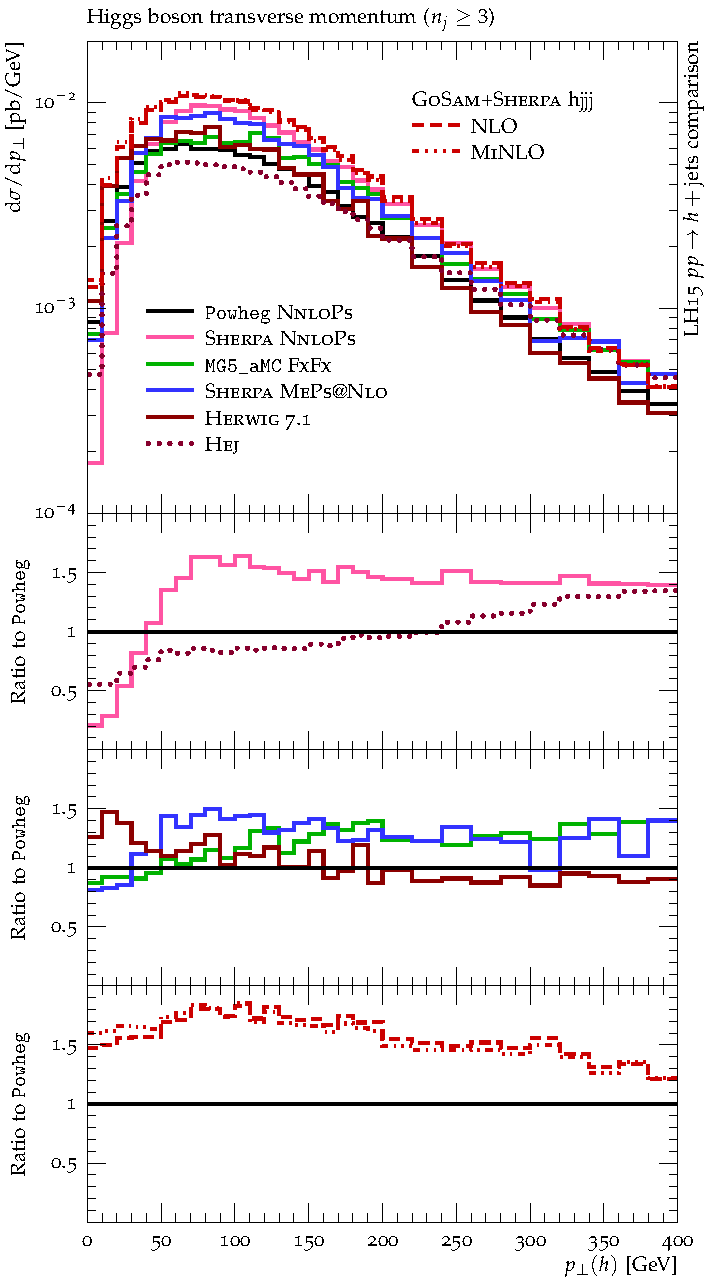
\includegraphics[width=0.47\textwidth]{figures/hjetscomp_u_H_jjj_pT_incl.pdf}
  \hfill
  \includegraphics[width=0.47\textwidth]{figures/hjetscomp_H_jjj_pT_incl.pdf}
  \caption{
    The Higgs boson transverse momentum in the presence of at least three 
    jets, shown without (left) and with (right) theoretical uncertainties.
    \label{fig:hjetscomp:results:mobs:hpt_j3}
  }
\end{figure}

The Higgs boson transverse momentum distribution for $H+\ge3$ jets is
shown in Figure~\ref{fig:hjetscomp:results:mobs:hpt_j3}. MG5 and
Sherpa tend to be higher than Powheg (where the jet is produced by a
parton shower), and similar to that from Gosam $H+\ge3$ jets, which
has the correct NLO $K$-factor.

\begin{figure}[t!]
  \centering
  \includegraphics[width=0.47\textwidth]{figures/hjetscomp_u_jet3_pT_incl.pdf}
  \hfill
  \includegraphics[width=0.47\textwidth]{figures/hjetscomp_jet3_pT_incl.pdf}
  \caption{
    The third jet transverse momentum distribution for $H+\ge3$ jets
    shown without (left) and with (right) theoretical uncertainty bands.
    \label{fig:hjetscomp:results:mobs:j3pt}
  }
\end{figure}

The third jet $p_T$ for $H+\ge3$ jets is shown in
Figure~\ref{fig:hjetscomp:results:mobs:j3pt}. MG5, Herwig7 and Sherpa
tend to be higher than Powheg (where the jet is produced by a parton
shower), but lower than that from Gosam $H+\ge3$ jets, which has the
correct NLO $K$-factor. The multijet phase space results in smaller
Sudakov effects, and thus better agreement with the fixed-order
predictions.

\begin{figure}[t!]
  \centering
  \includegraphics[width=0.47\textwidth]{figures/hjetscomp_u_HT_all.pdf}
  \hfill
  \includegraphics[width=0.47\textwidth]{figures/hjetscomp_HT_all.pdf}
  \caption{
    The $H_T$ distribution for $H+\ge1$ jets \Todo{is this correct?}
    without (left) and with (right) uncertainties.
    \label{fig:hjetscomp:results:mobs:HT_all}
  }
\end{figure}

\begin{figure}[t!]
  \centering
  \includegraphics[width=0.47\textwidth]{figures/hjetscomp_u_HT_jets.pdf}
  \hfill
  \includegraphics[width=0.47\textwidth]{figures/hjetscomp_HT_jets.pdf}
  \caption{
    The $H_{T,\mathrm{jets}}$ distribution for $H+\ge1$ jet final
    states, without (left) and with (right) uncertainties.
    \label{fig:hjetscomp:results:mobs:HT_jets}
  }
\end{figure}

The $H_T$ distribution (sum of the transverse momenta for all objects
in the final state) for $H+\ge1$ jets is shown in
Figure~\ref{fig:hjetscomp:results:mobs:HT_all} and the $H_T$
distribution for jets only is shown in in
Figure~\ref{fig:hjetscomp:results:mobs:HT_jets}. \Todo{Jan: we don't
  consider $H$ decays, so the all-objects HT would be different from
  an experimental point of view. Do we want both HTs and clarify or
  only the HTjets.}
MG5 and Sherpa tend to be lower than Powheg at low $H_T$ and higher at
large $H_T$. The fixed order predictions (from gosam and from $H+\ge1$
jet at NNLO) are consistently lower than Powheg (although the NNLO
prediction does agree with Powheg in the 150-300 GeV range for
$HT_{jets}$).



\clearpage
\subsection{Jet veto cross sections}
\label{sec:hjetscomp:results:jvobs}


In this section, we investigate jet veto cross sections, where the phase space for
additional gluon radiation is suppressed by means of a jet veto. 
%This section is concerned with the cummulative jet veto cross sections. 
In  Figures 
\ref{fig:hjetscomp:results:jvobs:jvxs0}-\ref{fig:hjetscomp:results:jvobs:jvxs1j200}, 
additional radiation has been vetoed by the application of a maximal transverse 
momentum for the (sub)leading jet, $p_\perp^\text{veto}$. The observables plotted
in the figures recover the respective inclusive cross sections as 
$p_\perp^\text{veto}\to\infty$. In this region, the fixed order 
part of the respective calculations dominates the cross section 
and associated uncertainties. The opposite regime, where $p_\perp^\text{veto}\to 0$, 
is a classic example of a resummation-dominated observable. Here, the 
properties of the respective parton showers come fully into play and 
differences are largely due to their separate characteristics. 
%The last case 
%investigated is cross section after VBF cuts when vetoing additional 
%central jet activity in dependence of the rapidity distance of the 
%tagging jet pair, $y_\text{dist}<y_\text{dist}^\text{max}$. Here, 
%DGLAP-type resummation regions are present throughout the spectrum and 
%this observable should be ideal to study BFKL-like dynamics.

\begin{figure}[t!]
  \centering
  \includegraphics[width=0.47\textwidth]{figures/hjetscomp_u_xs_jet_veto_j0.pdf}
  \hfill
  \includegraphics[width=0.47\textwidth]{figures/hjetscomp_xs_jet_veto_j0.pdf}
  \caption{
    The exclusive zero jet cross section as a function of 
    the vetoed minimal leading jet transverse momentum,
    without (left) and with (right) uncertainties.
    \label{fig:hjetscomp:results:jvobs:jvxs0}
  }
\end{figure}

We start by considering 
the cross section for the production of a Higgs boson and no 
additional jets, as a function of the minimum jet transverse momentum 
as shown in Figure~\ref{fig:hjetscomp:results:jvobs:jvxs0}. Remarkable 
agreement between both \NNLOPS simulations and the dedicated resummation 
calculations of STWZ is found, typically better than 5\% within the considered range. 
However, as the resummation accuracy for both \NNLOPS' implementations is limited by their parton 
shower's accuracy and they do not (\Powheg) or only partially (\Sherpa) 
assess their intrinsic resummation uncertainties and the interplay with the hard process 
scale variations, their uncertainties are less well-determined than those of STWZ. Although
the uncertainties for STWZ are similar to those of the \NNLOPS predictions for low values of the
jet veto transverse momentum, they are significantly smaller for higher values, perhaps reflecting the
effects of the $\pi^2$ resummation effects included in STWZ.
 The multijet merged predictions have a wider variation, and have veto cross sections lower than
that provided by the STWZ and the NNLOPS predictions. In addition to 
suffering from their NLO normalisation in the $p_\perp^\text{veto}\to\infty$ 
limit, they also show different behaviour as $p_\perp^\text{veto}\to 0$. For example, 
\Sherpa \MEPSatNLO exhibits more QCD activity than the other computations. 

\begin{figure}[t!]
  \centering
  \includegraphics[width=0.47\textwidth]{figures/hjetscomp_u_xs_jet_veto_j1_30.pdf}
  \hfill
  \includegraphics[width=0.47\textwidth]{figures/hjetscomp_xs_jet_veto_j1_30.pdf}
  \caption{
    The cross section for events containing a Higgs boson 
    and one jet with $p_\perp>30\,\gev$ as a function of
    the vetoed minimal second jet transverse momentum without
    (left) and with (right) uncertainties.
    \label{fig:hjetscomp:results:jvobs:jvxs1j30}
  }
\end{figure}

\begin{figure}[t!]
  \centering
  \includegraphics[width=0.47\textwidth]{figures/hjetscomp_u_xs_jet_veto_j1_200.pdf}
  \hfill
  \includegraphics[width=0.47\textwidth]{figures/hjetscomp_xs_jet_veto_j1_200.pdf}
  \caption{
    The cross section for events containing a Higgs boson 
    and one jet with $p_\perp>200\,\gev$ as a function of
    the vetoed minimal second jet transverse momentum without
    (left) and with (right) uncertainties.
    \label{fig:hjetscomp:results:jvobs:jvxs1j200}
  }
\end{figure}

Next, we require the presence of at least one jet with 
a minimal transverse momentum of either $30$ or $200$ \gev. 
The cross sections as a function of 
the sub-leading jets’ maximal transverse momentum are displayed in 
Figure~\ref{fig:hjetscomp:results:jvobs:jvxs1j30} and 
Figure~\ref{fig:hjetscomp:results:jvobs:jvxs1j200} for the two lead jet cuts. 
Note that, although all parton 
shower matched or merged calculations have the same accuracy both as 
$p_\perp^\text{veto}\to\infty$ and in the resummation dominated region, 
the multijet merged calculations possess a better description of the 
second jet emission, and thus should lead to more accurate results 
throughout the spectrum, provided the merging systematics are under control. 
Currently employed uncertainty estimates, however, will not reflect this 
as resummation uncertainties are not assessed or only incompletely assessed.

If we put no special requirements on the leading jet, cf.\ Figure 
\ref{fig:hjetscomp:results:jvobs:jvxs1j30}, good agreement 
between all calculations is found. The \NNLOPS predictions agree again within 
5\% of one another and have very similar uncertainties. This is noteworthy 
in sofar as, in comparison with the results of 
Figure~\ref{fig:hjetscomp:results:jvobs:jvxs0}, both calculations' 
accuracies are degraded by one order. The multijet merged calculations 
show similar behaviours as in the previous case: \MGaMC exhibits a smaller cross section due to 
its scale choice while \Sherpa \MEPSatNLO predicts more soft radiation. 
The relative lack of small $p_\perp$ radiation is more 
pronounced in \Herwig for this observable. Again, the uncertainties of \MGaMC and \Sherpa 
are of similar size while those of \Herwig are somewhat smaller than those of the \NNLOPS 
predictions, especially in the resummation-dominated region 
$p_\perp^\text{veto}\to 0$.

Raising the requirements on the leading jet to $200$ \gev, in Figure 
\ref{fig:hjetscomp:results:jvobs:jvxs1j200}, displays clear distinctions 
between the different calculations.  
\Sherpa \NNLOPS and \Powheg \NNLOPS have noticeably different shapes, with \Sherpa having a 
much lower cross section for low values of the sub-leading jet veto requirement. 
%starts out at a higher asymtotic cross section but remains within 
%20\% and of \Powheg, the respective uncertainties covering one another. 
The multijet merged calculations show \Herwig largely agreeing with 
\Powheg with a constant offset of $-10\%$, and the familiar lower 
probability of low-$p_\perp$ jet emissions. 
The asymptotic cross section for \Sherpa \MEPSatNLO is similar to that from \Sherpa \NNLOPS and, 
unsurprisingly, due to the use of the same parton shower, shows a 
similar radiation pattern. As before, it exhibits 
a relative overabundance of soft jet radiation. Lastly, the asymptotic cross section from \MGaMC 
is the same level as \Powheg's, despite 
its higher scale choice. The pattern of the uncertainties, however, 
remains the same as before.

%\Todo{The central jet veto cross sections are a mess. Looking into the 
%      analysis this is Ivan's code. It defines $y_\text{dist}$ as the 
%      minimal rapidity distance between the centre of the forward and 
%      backward jets and any jet inbetween,
%      $$
%	y_\text{dist}\;=\;\min\limits_{j|y(j_\text{bw})<y(j)<y(j_\text{fw})}
%	                  \left|y(j)-\frac{y_\text{fw}+y_\text{bw}}{2}\right|\;.
%      $$
%      It can thus take the maximum value of $4.4$. The cummulative cross 
%      section is then defined as 
%      $\sigma_2(y_\text{dist}>y_\text{dist}^\text{min})$. Thus, this 
%      observable vetoes events with too central additional radiation. 
%      It has one flaw in the implementation, however, in the absence of 
%      any third jet $y_\text{dist}$ is set to $>4.4$. Its asymtotic behaviour 
%      at large $y_\text{dist}$ converges thus to the exclusive VBF 
%      cross section, instead of zero. I just do not see what kind of 
%      dynamics we are probing or what kind of relevance a construction 
%      like this has. Especially since the forward backward jet are 
%      generally not the VBF tagging jets. We do also have the same observable 
%      in the pure dijet selection, which would then at least be nicely defined. 
%      Only the effects there are even smaller. 
%      Too many cooks, I guess. One should have had a recipe first.
%      }


% \begin{figure}[t!]
%   \centering
%   \includegraphics[width=0.47\textwidth]{figures/hjetscomp_u_xs_central_jet_veto_VBF.pdf}
%   \hfill
%   \includegraphics[width=0.47\textwidth]{figures/hjetscomp_xs_central_jet_veto_VBF.pdf}
%   \caption{
%     The cross section after VBF cuts as a function of the maximal minimum 
%     rapidity distance of a central jet to the centre of the most forward 
%     and most backward jet.
%     \label{fig:hjetscomp:results:jvobs:cjvxsvbf}
%   }
% \end{figure}
% 
% \begin{figure}[t!]
%   \centering
%   \includegraphics[width=0.47\textwidth]{figures/hjetscomp_u_xs_central_jet_veto_VBF2.pdf}
%   \hfill
%   \includegraphics[width=0.47\textwidth]{figures/hjetscomp_xs_central_jet_veto_VBF2.pdf}
%   \caption{
%     The cross section after generalised VBF cuts as a function of the maximal minimum 
%     rapidity distance of a central jet to the centre of the most forward 
%     and most backward jet.
%     \label{fig:hjetscomp:results:jvobs:cjvxsvbf2}
%   }
% \end{figure}
% 
% Finally, we consider the cross section after VBF cuts applying a veto 
% on additional central jet activity with $p_\perp>30\,\gev$ in dependence 
% of the maximal rapidity distance of the tagging jets, 
% $y_\text{dist}<y_\text{dist}^\text{max}$, as displayed in 
% Figure \ref{fig:hjetscomp:results:jvobs:cjvxsvbf}. Here, all parton shower based 
% resummation calculations give very similar results with \MGaMC possessing 
% a reduced cross section due to its scale choice. \Hej, being based on 
% BFKL dynamics, does not deviate substantially in its predicted shape. 
% However, its cross section is reduced by a constant 50-60\%. Alternatively, 
% when applying the generalised version of the VBF cuts, labelled VBF2, 
% a similar picture presents itself in 
% Figure \ref{fig:hjetscomp:results:jvobs:cjvxsvbf2}. While, of course, the 
% asymtotic cross section at large $y_\text{dist}^\text{max}$ coincides with 
% the one of the standard VBF cuts, for small $y_\text{dist}^\text{max}$ the 
% generalised VBF cuts allow for a much larger cross section.




\section{CONCLUSIONS}
\label{sec:hjetscomp:conclusions}

Precision Higgs boson measurements will soon be possible using the new
13 TeV data currently being collected during Run II of the LHC.
The largest Higgs boson production process is gluon fusion. A variety of theoretical 
tools exist for predictions for Higgs boson (+jets) production in this 
channel. As higher order corrections are especially sizable for $gg\to h$, 
it is important to understand the accuracies and regions of applicability 
of the various predictions. Too often, the comment has been that since 
the predictions agree within the theoretical uncertainties, all is well. 
However, a higher standard must be used, as the predictions have many of 
the theoretical uncertainties, such as scale uncertainties, in common. 

We have compared fixed order predictions at NLO and NNLO (including 
approximate NNLO), resummed predictions, NNLO predictions matched to parton 
showers, multjet merged predictions at NLO accuracy, and resummations 
in the BFKL limit. This allows a better understanding of two main issues: firstly how 
consistent are calculations which should be consistent and secondly the impact 
of soft gluon radiation and higher order corrections. All predictions have 
been carried out without non-perturbative corrections to allow for a one-to-one 
comparisons. A few observations follow. 

NNLO effects can change not only the normalization of distributions, but 
also the shape. For example, NLO predictions of the Higgs rapidity 
distribution are all similar in normalization and shape; however, the 
NLO predictions fall off more rapidly at high rapidity than predictions 
at NNLO. The differences between NLO and NNLO, however, are only 
noticeable in regions beyond the kinematic cuts applied at the LHC. It is 
interesting that, for the scale choices used in this study, there is 
neither a shape nor normalization shift from the NNLO corrections for the 
inclusive lead jet $p_\perp$ distribution while they are present for 
the Higgs boson $p_\perp$ in the presence of at least one jet.. 

The highest precision for inclusive jet multiplicity distributions is 
present with fixed order predictions, either at NLO or NNLO; in general, 
predictions from resummed/parton shower programs agree well with the 
fixed order predictions within their expected accuracy. The most 
extensive comparisons in this study are with respect to the $p_\perp$ 
distribution for the lead jet in $h+\ge1$ jet events. With the recent 
NNLO calculation for this quantity, the uncertainties are less than 10\%. 
As mentioned above, the NNLO corrections are small. The \NNLOPS 
predictions for this variable are in good agreement with each other 
as well as with the NLO/NNLO predictions for $p_\perp \le$ 100 GeV/c, with 
some separation between the \NNLOPS results at higher transverse momentum. 
The multijet jet merged predictions agree well with NLO/NNLO at low $p_\perp$, 
but fall below by about 15-20\% at high $p_\perp$. The jet veto resummed prediction from STWZ
agrees well at low $p_\perp$, but rises above the fixed order results 
by about 20\% at high $p_\perp$. One of the key take-home points is that 
the introduction of a parton shower or a resummation should not greatly 
affect the fixed order results, for observables that are suitably 
inclusive. These conclusions are largely true for comparisons for the 
sub-leading and third-leading jet as well. The situation is more complex 
for exclusive final states, where a jet veto is applied to any additional 
jet. Here, there are jet veto logs that have to be re-summed. We note, 
though, in general that there is still good agreement among the 
predictions used here. Although, this is not explicitly part of this 
study, we note that the impact of jet veto logarithms (after resummation) 
on the NNLO prediction for $h+\ge1$ jet are small, indicating again that 
the fixed order predictions for that quantity should be 
reliable~\cite{Banfi:2012jm,Banfi:2015pju}.

Resummed/parton shower predictions provide a better description for 
observables where Sudakov effects are important, such as the transverse 
momentum distribution for inclusive (exclusive) Higgs production. For 
the inclusive case, all predictions agree well with each other (and with 
the reference \HqT), with some deviations observed at the lowest $p_\perp$ 
values. Differences are more evident for the exclusive case, where the 
high transverse momentum for the Higgs boson must be supplied by a combination of 
jets lower than the $30\,\gev$ cutoff and soft gluon radiation. Although 
the fixed order predictions are unstable at low $p_\perp$, there is good 
agreement with the resummed/parton shower predictions at high $p_\perp$, 
where the bulk of the transverse momentum for the resummed/parton shower 
prediction is provided by the hard matrix element. 

In Sudakov regions involving multiple jets the situation gets more complex
and discrepancies often more evident. For example in looking at the 
Higgs boson $p_\perp$ distribution in $h+\ge n$ jet production, or the 
system $p_\perp$ for $h+n$ jets. It is interesting to note that the fixed 
order predictions are more stable at low transverse momentum when more 
jets are involved. 

The rapidity interval between two jets for $h+\ge2$ jets might be thought 
of as a fairly robust variable. However, differences can be observed among 
the various multijet merged predictions at high $\Delta y$. This is especially true 
if the two most forward-backward (rather than the two leading) jets are 
chosen, indicating perhaps that the differences in evidence are a result 
of the parton shower. It is interesting to note that the \Powheg \NNLOPS 
and \Sherpa \NNLOPS predictions agree well with each other and with the 
fixed order predictions (taking into account the NLO corrections present 
in the latter). The $\Delta \phi$ distribution between the two leading 
jets is an observable where basically all predictions agree. 

In order to measure the vector boson fusion process, additional kinematic 
cuts are necessary to reduce the gluon-gluon fusion background, requiring 
a dijet rapidity separation, and/or a dijet mass requirement, applied 
either to the leading jets (VBF) or to the two most forward-backwards 
jets (VBF2). The cross sections for $\ge2$ and $\ge3$ jets from \Sherpa 
\MEPSatNLO and from \GoSam{}+\Sherpa (with either of the VBF cuts) are larger than 
those from \Powheg \NNLOPS, expected as the normalizations for the $\ge2$ 
and $\ge3$ jet cross section for the former are at NLO. In general, the 
predictions for the kinematic distributions are similar among the various 
programs for both VBF and VBF2 cuts, except that both \Sherpa \MEPSatNLO and 
\Sherpa \NNLOPS tend to fill in the dip that occurs in the $\Delta \phi$ 
distribution at values around 1.5. The effect is larger when the 
forward-backward tagging is used, as might be expected if the effect was 
primarily due to the parton shower. 

A multi-jet quantity such as $H_{T, {\rm jets}}$ is sensitive to 
radiation/production of extra jets. Basically, all programs, with the 
exception of \Herwig, predict larger cross section than \Powheg \NNLOPS. 
The largest deviations are from the NNLO  $h+\ge1$ jet prediction, at 
$H_{T, {\rm jets}}$ values roughly from $200\,\gev$ to $400\,\gev$. 
It is interesting that the \Loopsim (nNLO) prediction for the same quantity 
is in good agreement with the exact NNLO prediction, as expected from the 
\Loopsim procedure.

Finally, we conclude with a brief review of the results from the jet veto 
cross section comparisons. For $h$ + no jets, the \NNLOPS predictions are 
in remarkable agreement with those obtained from STWZ. There is a wider 
variation from the multijet merged programs, with all predicting a smaller 
jet veto cross section than STWZ and the \NNLOPS programs. For $h$ plus 
exactly one jet ($\ge 30\,\gev$), the two \NNLOPS predictions are still in 
agreement with each other, and with the multijet predictions, with some 
divergence as the jet veto threshold is reduced below $30 \,\gev$. If the 
lead jet threshold is increased to $200\,\gev$, there is a wide divergence 
of predictions, indicating the difficulties of dealing with such multi-scale 
situations. 


\section*{ACKNOWLEDGEMENTS}

We thank the organisers.
MS acknowledges support by the Swiss National Science Foundation (SNF) 
under contract PP00P2-128552. 
The work of SH, YL and SP was supported by the U.S. Department of Energy 
under contract DE--AC02--76SF00515.


\bibliography{hjetscomp_bib}

\end{document}
